%================================================================
%  KHÓA LUẬN TỐT NGHIỆP
%  HỆ THỐNG PHÁT HIỆN CẢM XÚC DỰA TRÊN VĂN BẢN TIẾNG VIỆT
%  TÍCH HỢP VÀO CÁC NỀN TẢNG VIDEO CONFERENCING
%================================================================
% A4 undergraduate thesis layout.
\documentclass[13pt, a4paper, oneside]{extreport}

%----------------------------------------------------------------
% PACKAGES
%----------------------------------------------------------------
% Compile with XeLaTeX.  Fontspec embeds Unicode OpenType fonts directly,
% avoiding the broken Vietnamese glyphs produced by the legacy Type 1 times
% package in some PDF viewers.
\usepackage{fontspec}
\usepackage[vietnamese]{babel}
\setmainfont{TeX Gyre Termes}
\setsansfont{TeX Gyre Heros}
\setmonofont{TeX Gyre Cursor}
\usepackage{geometry}
\usepackage{graphicx}
\usepackage{float}
\usepackage{caption}
\usepackage{subcaption}
\usepackage{booktabs}
\usepackage{tabularx}
\usepackage{longtable}
\usepackage{multirow}
\usepackage{array}
\usepackage{xcolor}
\usepackage{colortbl}
\usepackage{hyperref}
\usepackage{url}
\usepackage{xurl}                % cho phép ngắt dòng URL/DOI dài trong bibliography
\usepackage{enumitem}
\usepackage{fancyhdr}
\usepackage{titlesec}
\usepackage{tocloft}
\usepackage{setspace}
\usepackage{indentfirst}
\usepackage{amsmath}
\usepackage{amssymb}
\usepackage{algorithm}
\usepackage{algpseudocode}
\usepackage{listings}
\usepackage{mdframed}
\usepackage{tikz}
\usepackage{pgfplots}
\usepackage{pgfplotstable}
\usepackage{appendix}
\usepackage{pdfpages}
\usepackage{footnote}
\usepackage{etoolbox}
\usepackage{fontawesome5}

\pgfplotsset{compat=1.18}

%----------------------------------------------------------------
% PAGE GEOMETRY (A4 thesis standard: left/right/top/bottom = 3.5/2/2.5/2.5 cm)
%----------------------------------------------------------------
\geometry{
  a4paper,
  top=25mm,
  bottom=25mm,
  left=35mm,    % lề trái rộng hơn để đóng bìa
  right=20mm
}

% Give TeX limited extra flexibility for Vietnamese prose mixed with immutable
% technical identifiers.  This prevents text from crossing the right margin
% without changing the document's declared body size.
\setlength{\emergencystretch}{6em}

%----------------------------------------------------------------
% LINE SPACING
%----------------------------------------------------------------
\setstretch{1.5}
\setlength{\parindent}{1cm}
\setlength{\parskip}{0pt}
\usetikzlibrary{arrows.meta, fit, positioning, backgrounds, calc, shapes.geometric}
%----------------------------------------------------------------
% COLORS
%----------------------------------------------------------------
\definecolor{primaryblue}{RGB}{31,78,121}
\definecolor{accentblue}{RGB}{41,128,185}
\definecolor{lightblue}{RGB}{213,232,240}
\definecolor{warningred}{RGB}{204,0,0}
\definecolor{notecolor}{RGB}{204,0,0}
\definecolor{codegray}{RGB}{245,245,245}
\definecolor{codecomment}{RGB}{106,153,85}
\definecolor{codestring}{RGB}{206,145,120}
\definecolor{codekeyword}{RGB}{86,156,214}
\definecolor{rowgray}{RGB}{242,242,242}

%----------------------------------------------------------------
% HYPERREF SETUP
%----------------------------------------------------------------
\hypersetup{
  colorlinks=true,
  linkcolor=primaryblue,
  citecolor=accentblue,
  urlcolor=accentblue,
  pdftitle={Hệ thống phân tích sắc thái cảm xúc từ transcript tiếng Việt trong họp trực tuyến},
  % Leave author metadata empty until the student supplies an identity; a
  % placeholder would be misleading in the distributed PDF.
  pdfauthor={},
  pdfsubject={Khóa luận tốt nghiệp},
  pdfkeywords={PhoBERT, phân tích sentiment, transcript tiếng Việt, thời gian thực, quyền riêng tư}
}
\urlstyle{same}

%----------------------------------------------------------------
% CHAPTER / SECTION TITLE FORMAT
%----------------------------------------------------------------
\titleformat{\chapter}[display]
  {\normalfont\bfseries\fontsize{16pt}{19pt}\selectfont\centering}
  {\chaptertitlename\ \thechapter}{10pt}{\MakeUppercase}
\titlespacing*{\chapter}{0pt}{0pt}{18pt}

\titleformat{\section}
  {\normalfont\bfseries\fontsize{14pt}{17pt}\selectfont}
  {\thesection}{1em}{}

\titleformat{\subsection}
  {\normalfont\bfseries\fontsize{13pt}{16pt}\selectfont}
  {\thesubsection}{1em}{}

\titleformat{\subsubsection}
  {\normalfont\normalsize\itshape}
  {\thesubsubsection}{1em}{}

%----------------------------------------------------------------
% HEADER / FOOTER
%----------------------------------------------------------------
\pagestyle{fancy}
\setlength{\headheight}{17pt}
\fancyhf{}
\fancyfoot[C]{\thepage}
\renewcommand{\headrulewidth}{0pt}
\renewcommand{\footrulewidth}{0pt}

% Plain style for chapter opening pages
\fancypagestyle{plain}{
  \fancyhf{}
  \fancyfoot[C]{\thepage}
  \renewcommand{\headrulewidth}{0pt}
}

%----------------------------------------------------------------
% TABLE OF CONTENTS
%----------------------------------------------------------------
\setcounter{tocdepth}{3}
\setcounter{secnumdepth}{3}

%----------------------------------------------------------------
% CODE LISTING STYLE
%----------------------------------------------------------------
\lstdefinestyle{pythonstyle}{
  backgroundcolor=\color{codegray},
  commentstyle=\color{codecomment},
  keywordstyle=\color{codekeyword}\bfseries,
  stringstyle=\color{codestring},
  basicstyle=\ttfamily\small,
  breakatwhitespace=false,
  breaklines=true,
  captionpos=b,
  keepspaces=true,
  numbers=left,
  numbersep=5pt,
  numberstyle=\tiny\color{gray},
  showspaces=false,
  showstringspaces=false,
  showtabs=false,
  tabsize=2,
  frame=single,
  rulecolor=\color{gray!30}
}

\lstdefinestyle{jsonstyle}{
  backgroundcolor=\color{codegray},
  basicstyle=\ttfamily\small,
  breaklines=true,
  frame=single,
  rulecolor=\color{gray!30},
  captionpos=b
}

\lstdefinestyle{bashstyle}{
  backgroundcolor=\color{black!90},
  basicstyle=\ttfamily\small\color{white},
  breaklines=true,
  frame=single,
  rulecolor=\color{black}
}

%----------------------------------------------------------------
% NOTE BOX (chú thích cần bổ sung)
%----------------------------------------------------------------
\newmdenv[
  topline=true,
  bottomline=true,
  rightline=true,
  leftline=true,
  leftmargin=5pt,
  rightmargin=5pt,
  innertopmargin=6pt,
  innerbottommargin=6pt,
  linecolor=warningred,
  linewidth=1.5pt,
  backgroundcolor=warningred!8,
  frametitle={\small\bfseries\color{warningred}\faExclamationTriangle\ GHI CHÚ CẦN BỔ SUNG},
  frametitleaboveskip=4pt
]{notebox}

%----------------------------------------------------------------
% FIGURE PLACEHOLDER BOX
%----------------------------------------------------------------
\newmdenv[
  topline=true,
  bottomline=true,
  rightline=true,
  leftline=true,
  linecolor=accentblue,
  linewidth=1pt,
  backgroundcolor=lightblue!30,
  innertopmargin=20pt,
  innerbottommargin=20pt,
  frametitle={\small\bfseries\color{accentblue}\faImage\ HÌNH VẼ CẦN BỔ SUNG},
  frametitleaboveskip=4pt
]{figurebox}

%----------------------------------------------------------------
% CUSTOM COMMANDS
%----------------------------------------------------------------
\newcommand{\todo}[1]{%
  \begin{notebox}
    \textit{#1}
  \end{notebox}%
}

\newcommand{\figplaceholder}[2]{%
  \begin{figurebox}
    \centering
    \textcolor{accentblue}{\large\textbf{#1}}\\[4pt]
    \textcolor{gray}{\small #2}
  \end{figurebox}%
}

\newcommand{\needvalue}[1]{\textcolor{warningred}{\textbf{[CẦN ĐIỀN: #1]}}}

%================================================================
% DOCUMENT BEGIN
%================================================================
\begin{document}

%----------------------------------------------------------------
% TRANG BÌA
%----------------------------------------------------------------
% The cover is intentionally unnumbered; enabling page anchors only after it
% avoids duplicate PDF destinations when Roman numbering begins at i.
\hypersetup{pageanchor=false}
% chapters/00_cover.tex
\begin{titlepage}
\begin{center}

{\large\bfseries TRƯỜNG ĐẠI HỌC GIAO THÔNG VẬN TẢI TP. HỒ CHÍ MINH}\\[6pt]
{\large\bfseries KHOA CÔNG NGHỆ THÔNG TIN}\\[4pt]
{\normalsize Ngành: Khoa học Máy tính \quad --- \quad Mã ngành: 8480101}

\vspace{2cm}

\textcolor{primaryblue}{\rule{\linewidth}{2pt}}\\[0.4cm]
{\Huge\bfseries\color{primaryblue} KHÓA LUẬN TỐT NGHIỆP}\\[0.4cm]
\textcolor{primaryblue}{\rule{\linewidth}{2pt}}

\vspace{1.5cm}

{\LARGE\bfseries\color{primaryblue}
HỆ THỐNG PHÂN TÍCH SẮC THÁI CẢM XÚC\\[6pt]
TỪ TRANSCRIPT TIẾNG VIỆT\\[6pt]
TRONG HỌP TRỰC TUYẾN
}

\vspace{2.5cm}

\begin{tabular}{ll}
  \textbf{Người hướng dẫn:}   & TS. Đặng Nhân Cách \\[8pt]
  \textbf{Sinh viên thực hiện:} & \needvalue{Họ và tên sinh viên} \\[4pt]
  \textbf{MSSV:}              & \needvalue{MSSV} \\[4pt]
  \textbf{Lớp:}               & \needvalue{Tên lớp} \\
\end{tabular}

\vfill

{\itshape TP. Hồ Chí Minh, tháng \needvalue{} năm \needvalue{}}

\end{center}
\end{titlepage}
\cleardoublepage

\hypersetup{pageanchor=true}

%----------------------------------------------------------------
% FRONT MATTER
%----------------------------------------------------------------
\pagenumbering{roman}
\setcounter{page}{1}

% chapters/00_declaration.tex
\chapter*{Lời Cam Đoan}
\addcontentsline{toc}{chapter}{Lời cam đoan}

Tôi xin cam đoan rằng khóa luận tốt nghiệp này là công trình nghiên cứu của riêng tôi dưới sự hướng dẫn của TS. Đặng Nhân Cách. Các kết quả trình bày trong khóa luận là trung thực, chưa được công bố trong bất kỳ công trình nghiên cứu nào khác.

Mọi tham khảo, trích dẫn trong khóa luận đều được ghi rõ nguồn gốc và tác giả theo quy định của nhà trường và tiêu chuẩn trích dẫn học thuật quốc tế (IEEE). Tôi hoàn toàn chịu trách nhiệm về tính trung thực, chính xác của nội dung luận văn này.

\vspace{2cm}
\begin{flushright}
  \textit{TP. Hồ Chí Minh, tháng \needvalue{} năm \needvalue{}}\\[1cm]
  \textit{Sinh viên thực hiện}\\[1.5cm]
  \textbf{\needvalue{Họ và tên}}
\end{flushright}
\cleardoublepage

\chapter*{Tóm Tắt}
\addcontentsline{toc}{chapter}{Tóm tắt}

\textbf{Bối cảnh:} Transcript do nhận dạng tiếng nói tự động tạo ra trong họp trực tuyến thường ngắn, nhiễu và có hiện tượng chuyển mã ngôn ngữ. Phân tích sắc thái cảm xúc trên nguồn dữ liệu này có thể hỗ trợ quan sát chất lượng trao đổi, nhưng không phải là cơ sở để suy luận hay chẩn đoán sức khỏe tâm thần của một cá nhân.

\textbf{Mục tiêu:} Khóa luận xây dựng một ứng dụng MVP xử lý transcript tiếng Việt trong họp trực tuyến, đồng thời thiết kế quy trình kiểm chứng có bằng chứng truy vết, bảo vệ quyền riêng tư và cập nhật gần thời gian thực. Ứng dụng được thiết kế để nhận một bộ phân loại sentiment có thể thay thế; đầu ra dự kiến gồm ba lớp \textit{positive}, \textit{neutral}, \textit{negative}; lớp \textit{unknown} được giữ lại khi dữ liệu hoặc bộ phân loại không đủ điều kiện.

\textbf{Phương pháp:} Hệ thống tiếp nhận transcript từ Jitsi Meet qua Vexa và dịch vụ STT cục bộ, lưu phiên bản segment trong backend sở hữu dữ liệu, áp dụng quality gate và language router, ghép các segment cùng người nói thành analysis unit, sau đó gọi adapter phân loại và tổng hợp theo cửa sổ thời gian. Kiến trúc dùng FastAPI, PostgreSQL, Valkey Stream, worker tách riêng và SSE. PhoBERT và custom model là lựa chọn tích hợp về mặt lý thuyết \cite{phobert2020}; runtime hiện thực của MVP là \texttt{baseline-rules-v3} để kiểm tra hợp đồng xử lý, không phải kết quả fine-tune hay đánh giá chất lượng mô hình.

\textbf{Kết quả:} Khóa luận báo cáo hai snapshot Dashboard local ngày 15/11/2026 ở mức quan sát (E1), không phải UAT pass: snapshot pilot hiển thị 116 segment, 38/39/39 unit predicted/accepted/total và coverage 97\%. Kho evidence cũng có một bundle integration synthetic E2 lịch sử cho \texttt{baseline-rules-v2}, không dùng để xác minh runtime hiện tại. Không công bố accuracy/F1 sentiment, WER ASR, độ trễ E2E, benchmark đa mô hình hay năng lực sàng lọc sức khỏe tâm thần. Dashboard hiển thị KPI, timeline, evidence và cập nhật SSE khi có dữ liệu chạy thực tế.

\textbf{Kết luận:} MVP tạo nền tảng có thể kiểm toán để tích hợp bộ phân loại sentiment vào transcript họp. Huấn luyện lại, benchmark, calibration và đánh giá trải nghiệm là hướng tối ưu hóa tiếp theo, không phải đóng góp thực nghiệm của khóa luận này.

\vspace{0.5cm}
\textbf{Từ khóa:} \textit{Phân tích sentiment, PhoBERT, transcript tiếng Việt, họp trực tuyến, event-driven, evidence, quyền riêng tư.}

\vspace{1cm}
\hrule
\vspace{0.5cm}

\chapter*{Abstract}
\addcontentsline{toc}{chapter}{Abstract}

\textbf{Background:} Automatic-speech-recognition transcripts from online meetings are often short, noisy, and code-switched. Sentiment analysis can assist the observation of conversational content, but it must not be used to infer or diagnose an individual's mental health.

\textbf{Objective:} This thesis builds an application MVP for Vietnamese meeting transcripts and defines an evidence-traceable, privacy-aware, near-real-time verification process. The application is designed to accept a replaceable sentiment classifier. The intended task comprises \textit{positive}, \textit{neutral}, and \textit{negative} classes; \textit{unknown} is retained when data or classifier conditions are insufficient.

\textbf{Methods:} The system ingests Jitsi Meet transcripts through Vexa and a local STT service, versions segments in an application-owned backend, applies a quality gate and language router, constructs speaker-bounded analysis units, invokes a classifier adapter, and publishes windowed aggregates. FastAPI, PostgreSQL, Valkey Stream, a separate worker, and SSE form the implementation. PhoBERT and custom models are theoretical integration options \cite{phobert2020}; the implemented MVP runtime is \texttt{baseline-rules-v3}, which exercises the processing flow rather than claiming a fine-tuned-model evaluation.

\textbf{Results:} The thesis reports two local Dashboard snapshots dated 15 November 2026 as E1 observations, not UAT passes. The pilot snapshot displays 116 segments, 38/39/39 predicted/accepted/total units, and 97\% coverage. The evidence store also contains one historical E2 synthetic-integration bundle for \texttt{baseline-rules-v2}; it does not validate the current runtime. No sentiment accuracy/F1, ASR WER, end-to-end latency, multi-model benchmark, or mental-health-screening capability is reported. The dashboard displays KPIs, a timeline, evidence, and SSE updates when runtime data are available.

\textbf{Keywords:} \textit{Sentiment analysis, PhoBERT, Vietnamese transcript, online meeting, event-driven architecture, evidence, privacy.}

\cleardoublepage


\tableofcontents
\listoftables
\listoffigures
% chapters/00_acronyms.tex
\chapter*{Danh Mục Từ Viết Tắt}
\addcontentsline{toc}{chapter}{Danh mục từ viết tắt}

\begin{longtable}{>{\bfseries}p{3cm} p{11cm}}
\toprule
\textbf{Viết tắt} & \textbf{Nghĩa đầy đủ} \\
\midrule
\endhead
\bottomrule
\endfoot
AI       & Artificial Intelligence -- Trí tuệ nhân tạo \\[4pt]
API      & Application Programming Interface \\[4pt]
ASR      & Automatic Speech Recognition -- Nhận dạng giọng nói tự động \\[4pt]
BERT     & Bidirectional Encoder Representations from Transformers \\[4pt]
BPE      & Byte-Pair Encoding \\[4pt]
GDPR     & General Data Protection Regulation -- Quy định bảo vệ dữ liệu chung của EU \\[4pt]
MLM      & Masked Language Modeling \\[4pt]
NLP      & Natural Language Processing -- Xử lý ngôn ngữ tự nhiên \\[4pt]
REST     & Representational State Transfer \\[4pt]
SSE      & Server-Sent Events \\[4pt]
TLS      & Transport Layer Security \\[4pt]
WER      & Word Error Rate -- Tỷ lệ lỗi từ \\
\end{longtable}
\cleardoublepage


%----------------------------------------------------------------
% MAIN MATTER
%----------------------------------------------------------------
\pagenumbering{arabic}
\setcounter{page}{1}

\chapter{Giới Thiệu}
\label{chap:intro}

\section{Bối cảnh và tính cấp thiết của nghiên cứu}
Sự phổ biến của họp trực tuyến làm cho một lượng lớn trao đổi công việc và học tập được chuyển thành dữ liệu âm thanh. Khi kết hợp với nhận dạng tiếng nói tự động (Automatic Speech Recognition -- ASR), các trao đổi này có thể được biểu diễn dưới dạng transcript để tìm kiếm, rà soát và phân tích. Các mô hình ASR hiện đại đã cho thấy khả năng hoạt động trên nhiều ngôn ngữ và điều kiện âm thanh nhờ huấn luyện quy mô lớn \cite{whisper2022}. Tuy nhiên, transcript sinh tự động không phải bản ghi chép hoàn hảo: tiếng ồn nền, chồng lấn lời nói, lỗi phân tách người nói, phát ngôn ngắn và hiện tượng chuyển mã Việt--Anh đều có thể làm thay đổi hoặc làm thiếu ngữ cảnh của văn bản đầu vào.

Trong bối cảnh đó, phân tích sắc thái cảm xúc (sentiment analysis) có thể hỗ trợ người dùng quan sát xu hướng biểu đạt của \emph{nội dung trao đổi}, chẳng hạn tỷ trọng phát ngôn tích cực, trung tính hoặc tiêu cực theo thời gian. Với tiếng Việt, các mô hình ngôn ngữ tiền huấn luyện như PhoBERT là một lựa chọn đáng chú ý cho các tác vụ xử lý ngôn ngữ tự nhiên \cite{phobert2020}. Dù vậy, năng lực của mô hình ngôn ngữ không loại bỏ các vấn đề thuộc hệ thống: dữ liệu vào cần được kiểm soát chất lượng, kết quả phải liên kết được với segment nguồn và thay đổi của transcript không được làm mất lịch sử phân tích.

Vì thế, giá trị của một ứng dụng trong miền này không chỉ nằm ở việc gọi một bộ phân loại. Hệ thống cần phân tách rõ dữ liệu thô, dữ liệu đủ điều kiện để suy luận và kết quả tổng hợp; đồng thời lưu phiên bản transcript, phiên bản mô hình, confidence, coverage và evidence để người dùng có thể kiểm tra ngữ cảnh của mỗi kết quả. Cách tiếp cận này phù hợp với nguyên tắc bảo vệ dữ liệu ngay từ thiết kế (privacy by design) \cite{cavoukian2011} và nguyên tắc tối thiểu hóa dữ liệu trong GDPR \cite{gdpr2016}.

Một ranh giới khoa học và đạo đức đặc biệt quan trọng là không đồng nhất sentiment với trạng thái sức khỏe tâm thần. Nhãn tích cực, trung tính hoặc tiêu cực của một analysis unit chỉ mô tả sắc thái của văn bản trong ngữ cảnh hẹp; nó không phải bằng chứng về đặc điểm, năng lực hay bệnh lý của người nói. Trầm cảm là tình trạng cần được đánh giá theo tiêu chí lâm sàng; PHQ-9 là công cụ tự báo cáo trong một khoảng thời gian xác định \cite{kroenke2001}, còn chẩn đoán đòi hỏi đánh giá chuyên môn theo các tiêu chuẩn như DSM-5 \cite{dsm5}. Do đó, khóa luận không phát hiện hay sàng lọc trầm cảm, không xếp hạng cá nhân và không hỗ trợ quyết định về học tập, tuyển dụng hoặc việc làm.

\section{Vấn đề nghiên cứu}
Từ bối cảnh trên, bài toán được đặt ra là: làm thế nào xây dựng một MVP phân tích sentiment từ transcript tiếng Việt trong họp trực tuyến mà vẫn bảo toàn khả năng truy vết, thay thế mô hình và kiểm soát cách diễn giải đầu ra? Bài toán được cụ thể hóa thành bốn vấn đề thiết kế và hiện thực:
\begin{enumerate}[label=(\roman*)]
  \item lọc các segment rỗng, quá ngắn, chưa hoàn tất, bị thu hồi hoặc có mẫu hallucination đã biết; lưu lại lý do loại thay vì âm thầm bỏ dữ liệu;
  \item thiết kế hợp đồng adapter để bộ phân loại có thể được thay thế mà không làm thay đổi API, persistence và dashboard;
  \item bảo toàn transcript gốc, revision và vòng đời phân tích trong kiến trúc cập nhật gần thời gian thực;
  \item trình bày evidence, confidence và coverage để đầu ra được hiểu là hỗ trợ quan sát nội dung, không phải kết luận về con người.
\end{enumerate}

Các vấn đề này gắn trực tiếp với kiến trúc của dự án. Ở runtime hiện hành, Jitsi Meet là nguồn cuộc họp WebRTC, Vexa cung cấp bot và transcript, còn ứng dụng sở hữu bản sao transcript, phiên bản phân tích và dashboard:
\begin{center}
\texttt{Jitsi Meet $\rightarrow$ Vexa bot $\rightarrow$ STT local $\rightarrow$ FastAPI/PostgreSQL $\rightarrow$ Valkey Stream $\rightarrow$ worker $\rightarrow$ SSE Dashboard.}
\end{center}
PostgreSQL là nguồn dữ liệu chuẩn; Valkey Stream chỉ phục vụ hàng đợi và fan-out, không thay thế dữ liệu bền vững. Worker tách khỏi FastAPI để suy luận không chặn API, còn dashboard chỉ giao tiếp với backend nên không tiếp xúc với khóa API của nhà cung cấp transcript. Cách phân tách này đồng thời tạo điều kiện kiểm toán lại chuỗi xử lý.

Kiến trúc được định hướng theo mô hình đa nền tảng. Bên ngoài lõi ứng dụng, mỗi nền tảng họp---Jitsi Meet, Google Meet, Microsoft Teams hoặc Zoom---cần một \emph{platform adapter} chịu trách nhiệm xác thực URL/lịch họp, khởi tạo bot hoặc kết nối thu âm theo quyền được cấp, và chuẩn hóa transcript về cùng hợp đồng gồm định danh cuộc họp, speaker, timestamp, text, trạng thái \texttt{is\_final} và revision. Sau bước chuẩn hóa, mọi dữ liệu đi qua cùng quality gate, worker, persistence và dashboard; vì vậy việc thêm platform không làm thay đổi ngữ nghĩa của dữ liệu phân tích. Trong phiên bản hiện tại, adapter Jitsi kết hợp Vexa và STT local là đường runtime đã cấu hình. Adapter cho Google Meet, Teams và Zoom vẫn cần contract nguồn, cơ chế consent, kiểm thử tích hợp và đánh giá riêng trước khi được nêu là hỗ trợ.

\section{Mục tiêu, câu hỏi và phương pháp nghiên cứu}
\textbf{Mục tiêu tổng quát} là xây dựng và kiểm chứng ở mức tích hợp một ứng dụng có khả năng tiếp nhận transcript tiếng Việt trong họp trực tuyến, áp dụng bộ phân loại sentiment có thể thay thế, và cung cấp kết quả có bằng chứng truy vết cùng các cơ chế bảo vệ quyền riêng tư. Khóa luận không đặt mục tiêu huấn luyện lại mô hình hoặc chứng minh chất lượng dự báo của một mô hình học máy cụ thể.

Để đạt mục tiêu này, nghiên cứu sử dụng hướng thiết kế--hiện thực--kiểm chứng artefact phần mềm: xác định yêu cầu và ràng buộc; thiết kế hợp đồng dữ liệu và kiến trúc; hiện thực MVP; sau đó kiểm chứng các luồng ingest, xử lý, lưu vết và hiển thị. Hướng tiếp cận này tương thích với quan điểm nghiên cứu khoa học thiết kế trong hệ thống thông tin, nơi artefact được xây dựng và đánh giá để giải quyết một lớp vấn đề xác định \cite{hevner2004}. Đánh giá trong khóa luận là kiểm chứng kỹ thuật của MVP, không phải đánh giá lâm sàng hay benchmark hiệu năng mô hình.

\textbf{Câu hỏi nghiên cứu:}
\begin{enumerate}
  \item Pipeline có loại, lưu vết lý do và bảo toàn revision của transcript không đủ điều kiện trước khi gọi bộ phân loại hay không?
  \item Hợp đồng adapter có cho phép thay thế bộ phân loại hiện tại bằng PhoBERT hoặc model artifact phù hợp mà không thay đổi API, persistence và dashboard hay không?
  \item Kiến trúc event-driven có hoàn tất ingest, analysis lifecycle, persistence và cập nhật dashboard từ final segment hay không, đồng thời duy trì một hợp đồng có thể mở rộng sang platform adapter khác?
  \item Evidence, confidence và coverage trên dashboard được biểu diễn như thế nào để tránh coi output là kết luận về con người?
\end{enumerate}

\section{Đối tượng, phạm vi và giới hạn}
\textbf{Đối tượng nghiên cứu} là pipeline xử lý transcript và kiến trúc ứng dụng phân tích sentiment, không phải việc nhận dạng cảm xúc đa phương thức hay đánh giá sức khỏe tâm thần. Đơn vị xử lý là \emph{analysis unit} được ghép từ các final segment liền kề của cùng người nói, có giới hạn về số segment và thời gian. Baseline hiện hành nhận unit tiếng Việt hoặc tiếng Anh; unit trộn/ngôn ngữ không hỗ trợ, hoặc không đạt quality gate, giữ nhãn \textit{unknown}.

MVP được vận hành cục bộ với Jitsi Meet, Vexa và STT local. Runtime hiện hành là rule baseline có tính xác định, phiên bản \texttt{baseline-rules-v3}, hỗ trợ route Việt/Anh để kiểm tra data contract, luồng hàng đợi, persistence và dashboard; đây không phải mô hình học máy, không phải dịch máy và không được dùng để kết luận về chất lượng sentiment. Các notebook model sẵn có trong thư mục dự án chỉ phục vụ tham khảo hoặc khám phá. Đặc biệt, notebook phân loại trầm cảm nhị phân khác về task, nhãn và domain so với sentiment ba lớp của ứng dụng, nên không phải artifact được phục vụ trong MVP.

Hợp đồng \texttt{SentimentClassifier} mở đường cho \emph{custom model} (mô hình tùy biến) theo từng tổ chức, miền nghiệp vụ hoặc tập dữ liệu đã được cho phép sử dụng. Một custom model chỉ có thể được đưa vào vận hành khi được đóng gói thành artifact có định danh version, khai báo rõ task/nhãn/ngôn ngữ, tương thích với hợp đồng input--output và có báo cáo đánh giá trên tập dữ liệu phù hợp. Mỗi prediction cần lưu model version, preprocessing version và evidence để có thể tái lập, so sánh hoặc rollback. Cơ chế này không đồng nghĩa với việc huấn luyện mô hình trên transcript của người dùng: việc thu thập, gán nhãn hoặc fine-tune dữ liệu theo từng khách hàng chỉ được thực hiện khi có cơ sở pháp lý, consent, chính sách lưu giữ dữ liệu và đánh giá rủi ro riêng.

Do chưa có corpus transcript họp được gán nhãn đúng task và protocol đánh giá tương ứng, khóa luận không công bố macro-F1, accuracy, calibration, WER ASR, độ trễ percentile hay kết quả đánh giá người dùng. PhoBERT, custom model, benchmark đa mô hình, đo WER, Kubernetes, high availability và triển khai thực tế trên Google Meet, Zoom hoặc Teams là hướng phát triển tiếp theo. Khi có dữ liệu hợp pháp và đánh giá thực nghiệm, các kết quả đó cần được báo cáo theo protocol tách dữ liệu theo cuộc họp, giữ test set độc lập và nêu rõ phiên bản model/dữ liệu.

\section{Đóng góp của khóa luận}
Trong giới hạn nêu trên, khóa luận đóng góp một artefact MVP và các quyết định thiết kế có thể tái sử dụng cho bài toán tương tự:
\begin{itemize}
  \item một pipeline transcript có quality gate, định tuyến ngôn ngữ, ghép analysis unit theo người nói và lưu revision/evidence;
  \item một giao diện \texttt{SentimentClassifier} tách rời mô hình khỏi API, cơ sở dữ liệu và dashboard, tạo đường tích hợp có kiểm soát cho model artifact sau này;
  \item một kiến trúc event-driven với PostgreSQL là nguồn dữ liệu chuẩn, outbox/queue cho xử lý bất đồng bộ và SSE cho cập nhật dashboard;
  \item một adapter Jitsi dùng chung lõi phân tích với định hướng mở rộng sang Google Meet, Microsoft Teams và Zoom sau khi từng adapter được hiện thực và kiểm chứng;
  \item cách biểu diễn dashboard nhấn mạnh coverage, confidence, timeline và evidence, đi kèm ranh giới sử dụng nhằm giảm nguy cơ diễn giải quá mức.
\end{itemize}

\section{Cấu trúc khóa luận}
Chương~\ref{chap:literature} trình bày cơ sở lý thuyết và ranh giới giữa sentiment với sàng lọc lâm sàng. Chương~\ref{chap:data} mô tả dữ liệu, hợp đồng và pipeline phân tích; Chương~\ref{chap:model} nêu trạng thái mô hình, adapter và protocol đánh giá khi huấn luyện lại. Các Chương~\ref{chap:backend}--\ref{chap:infra} trình bày hiện thực MVP ở backend, frontend và hạ tầng. Chương~\ref{chap:experiments} báo cáo kiểm chứng tích hợp và giới hạn thực nghiệm; Chương~\ref{chap:ethics} phân tích bảo vệ dữ liệu cùng các ràng buộc đạo đức; cuối cùng, Chương~\ref{chap:conclusion} tổng kết và đề xuất hướng phát triển.

\chapter{Tổng Quan Nghiên Cứu và Cơ Sở Lý Thuyết}
\label{chap:literature}

Chương này hệ thống hóa các khái niệm cần thiết để thiết kế ứng dụng phân tích sentiment từ transcript họp trực tuyến. Trọng tâm là sự phù hợp giữa bài toán phân tích ngôn ngữ, chất lượng dữ liệu ASR và các cơ chế hệ thống để kết quả có thể truy vết. Các nội dung về mô hình, đa nền tảng và vận hành được trình bày như cơ sở thiết kế; chúng không thay thế bằng chứng thực nghiệm được báo cáo ở Chương~\ref{chap:experiments}.

\section{Sentiment analysis trong bối cảnh transcript họp}
\subsection{Khái niệm và đơn vị phân tích}
Sentiment analysis, hay opinion mining, là nhóm kỹ thuật xác định khuynh hướng đánh giá hoặc sắc thái biểu đạt trong văn bản \cite{pang2008}. Trong khóa luận này, bài toán được giới hạn ở phân loại polarity ba lớp \textit{positive}, \textit{neutral} và \textit{negative} trên một \emph{analysis unit}; lớp \textit{unknown} biểu thị dữ liệu không đủ điều kiện hoặc không thuộc miền/ngôn ngữ mà adapter hỗ trợ. Như vậy, \textit{unknown} là một trạng thái an toàn của hệ thống, không phải một lớp sentiment.

Việc chọn analysis unit thay vì một token, một câu đơn lẻ hoặc toàn bộ cuộc họp là quyết định thiết kế nhằm cân bằng ngữ cảnh và độ trễ. Một unit được xây dựng từ tối đa ba final segment liền kề của cùng người nói, trong giới hạn thời gian của pipeline. Cách ghép này có thể giữ lại phủ định hoặc bổ ngữ nằm ở segment lân cận, đồng thời không gom nhiều lượt thoại khác người nói vào cùng một dự đoán. Tuy nhiên, unit vẫn không đủ để diễn giải ý định, mỉa mai hoặc quan hệ xã hội; các hiện tượng đó chỉ có thể được đánh giá khi có guideline và dữ liệu gán nhãn phù hợp.

\subsection{Phân biệt các lớp bài toán}
Sentiment, emotion, intent và đánh giá lâm sàng có mục tiêu, nhãn và yêu cầu dữ liệu khác nhau. Sự phân biệt này cần được duy trì từ khâu thu thập dữ liệu đến giao diện người dùng để tránh suy diễn vượt quá bằng chứng.

\begin{table}[H]
\centering
\caption{Ranh giới giữa các lớp bài toán liên quan đến transcript}
\label{tab:task-boundary}
\begin{tabularx}{\linewidth}{p{0.19\linewidth}XX}
\toprule
Bài toán & Đầu ra/dữ liệu cần có & Quan hệ với khóa luận \\ \midrule
Sentiment & Polarity ở cấp analysis unit; guideline gán nhãn theo ngữ cảnh họp & Bài toán đích của kiến trúc ứng dụng \\
Emotion / intent & Nhiều nhãn cảm xúc hoặc mục đích phát ngôn; dữ liệu và guideline riêng & Hướng mở rộng, không suy ra từ nhãn sentiment \\
Tóm tắt/đánh giá cuộc họp & Ngữ cảnh nhiều lượt thoại, mục tiêu cuộc họp và tiêu chí đánh giá riêng & Không phải đầu ra của classifier hiện tại \\
Sàng lọc lâm sàng & Công cụ đã được thẩm định, khoảng thời gian xác định, consent và chuyên môn lâm sàng & Ngoài phạm vi \\ \bottomrule
\end{tabularx}
\end{table}

PHQ-9 là công cụ tự báo cáo trong một cửa sổ thời gian xác định \cite{kroenke2001}; chẩn đoán còn đòi hỏi đánh giá chuyên môn theo DSM-5 \cite{dsm5}. Vì vậy, không có phép ánh xạ trực tiếp từ sentiment của một transcript sang tiêu chí PHQ-9, DSM-5 hoặc trạng thái sức khỏe tâm thần của người nói. Hệ thống không được thiết kế để xếp hạng con người hoặc hỗ trợ quyết định học tập, tuyển dụng hay việc làm.

\section{Transcript ASR và kiểm soát chất lượng dữ liệu}
\subsection{Nguồn sai lệch của transcript}
ASR biến tín hiệu âm thanh thành chuỗi ký tự; các hệ thống hiện đại có thể hoạt động trên dữ liệu đa ngôn ngữ ở quy mô lớn \cite{whisper2022}. Tuy nhiên, chất lượng transcript còn chịu ảnh hưởng của tiếng ồn, vọng âm, lời nói chồng lấn, tốc độ nói, tên riêng, từ viết tắt, chuyển mã ngôn ngữ và lỗi diarization. Với họp trực tuyến, một lỗi nhỏ cũng có thể đảo polarity, ví dụ làm mất từ phủ định hoặc gán phát ngôn sang sai speaker. Do đó, transcript phải được xem là dữ liệu quan sát có sai số, không phải ground truth ngôn ngữ.

Khi có audio gốc và bản chép chuẩn tương ứng, Word Error Rate (WER) có thể được xác định bởi:
\begin{equation}
  WER = \frac{S + D + I}{N},
\end{equation}
trong đó $S$, $D$, $I$ lần lượt là số lỗi thay thế, xóa và chèn; $N$ là số từ trong bản chép chuẩn. Với tiếng Việt, việc định nghĩa token và quy tắc tách từ phải được cố định trước khi so sánh. WER/CER chỉ phản ánh sai khác so với ground truth đã chọn; chúng không trực tiếp đo đúng--sai của nhãn sentiment. Vì MVP chưa có audio và ground truth được thiết kế để benchmark, khóa luận không báo cáo WER/CER.

\subsection{Quality gate, language routing và coverage}
Trước suy luận, hệ thống chuẩn hóa Unicode NFC và khoảng trắng, đồng thời giữ nguyên dấu tiếng Việt. Quality gate đánh giá ít nhất các điều kiện: text rỗng, số từ quá ít, duration âm, segment chưa final, segment bị retracted và mẫu hallucination đã biết. Language router chỉ chuyển unit tiếng Việt đến adapter hiện hành; trường hợp khác hoặc không chắc chắn được giữ \textit{unknown}. Segment bị loại vẫn lưu text đã chuẩn hóa và lý do loại để có thể audit, thay vì bị xóa hoặc ép thành \textit{neutral}.

Để tránh diễn giải nhầm một tỷ lệ dự đoán cao là toàn bộ transcript đã được xử lý, hệ thống tách ba chỉ số. Với $T$ là tổng số đơn vị được xem xét trước quality gate, $A$ là số unit được chấp nhận và $P$ là số unit có nhãn khác \textit{unknown}, hệ thống định nghĩa:
\begin{equation}
  r_{\mathrm{accept}}=\frac{A}{T},\qquad
  r_{\mathrm{prediction}}=\frac{P}{A},\qquad
  r_{\mathrm{effective}}=\frac{P}{T}.
\end{equation}
Các tỷ lệ có mẫu số bằng 0 được báo là $0$ kèm trạng thái ``không có đơn vị phù hợp'', không được suy diễn thành tỷ lệ sentiment. \emph{Prediction coverage} thấp có thể do routing, ngưỡng confidence hoặc adapter; \emph{acceptance rate} thấp phản ánh chất lượng đầu vào; còn \emph{effective coverage} cho biết phần nội dung ban đầu thực sự nhận được dự đoán. Backend lưu cả ba chỉ số; dashboard hiện giữ \emph{prediction coverage} để tương thích và cần bổ sung hai chỉ số còn lại trước khi công bố kết quả vận hành.

\section{Nền tảng họp, bot và STT cục bộ}
Jitsi Meet là nguồn cuộc họp của runtime hiện tại, còn Vexa là control plane cho vòng đời bot và transcript. Theo tài liệu kiến trúc của Jitsi, ứng dụng họp dựa trên WebRTC, với Jitsi Videobridge định tuyến media, Jicofo điều phối phiên và Prosody phục vụ signalling \cite{jitsiArchitecture2026}. Các thành phần này thuộc miền hội nghị; backend của đề tài không thay thế chúng và không coi chúng là source of truth cho dữ liệu phân tích. Về phía bot/transcript, Vexa cung cấp quy trình tạo bot và lấy transcript, trong khi application vẫn phải lưu version/revision của bản sao được dùng cho phân tích \cite{vexaQuickstart2026}.

Sau khi bot thu nhận audio theo quyền được cấp, dịch vụ STT cục bộ giải mã audio thành segment trước khi pipeline sentiment chạy. Runtime dùng faster-whisper trên CTranslate2 với cấu hình CPU \texttt{int8} và VAD; các lựa chọn này hỗ trợ trade-off chi phí/tốc độ suy luận, không phải bằng chứng về độ chính xác transcript cho dữ liệu họp tiếng Việt \cite{fasterwhisper2026}. Vì ASR, diarization và dịch máy là ba bài toán khác nhau, hệ thống không diễn giải output STT như bản dịch hay cho rằng việc nhận diện được ngôn ngữ đồng nghĩa với chất lượng dịch. Mọi tuyên bố WER/CER vẫn cần audio, bản chép chuẩn và protocol đánh giá độc lập.

\section{Nền tảng mô hình ngôn ngữ và custom model}
\subsection{Các lựa chọn mô hình cho tiếng Việt}
Transformer dùng self-attention để biểu diễn quan hệ ngữ cảnh \cite{vaswani2017}:
\begin{equation}
\mathrm{Attention}(Q,K,V)=\mathrm{softmax}\left(\frac{QK^\top}{\sqrt{d_k}}\right)V.
\end{equation}
BERT là encoder Transformer được tiền huấn luyện bằng masked language modeling \cite{devlin2019}; PhoBERT là mô hình tiền huấn luyện chuyên cho tiếng Việt \cite{phobert2020}. Khi dùng PhoBERT, tokenizer, checkpoint và bước word segmentation phải tương thích; không áp dụng stemming hay loại stopword một cách mặc định vì có thể làm mất thông tin phủ định và ngữ cảnh.

TF--IDF kết hợp Logistic Regression, PhoBERT fine-tune và mBERT/XLM-R là các hướng so sánh hợp lý khi có dataset đúng task \cite{xlmr2020}. Không có mô hình nào mặc nhiên tốt nhất cho transcript họp: khác biệt về miền dữ liệu, cách ghi transcript, phân bố lớp và quy tắc gán nhãn có thể làm thay đổi kết quả. Vì vậy, PhoBERT trong khóa luận là một ứng viên tích hợp, không phải kết quả benchmark đã đạt.

\subsection{Hợp đồng adapter và vòng đời custom model}
Để tách phần hệ thống khỏi thuật toán, worker gọi giao diện \texttt{SentimentClassifier} thay vì phụ thuộc vào một framework mô hình cụ thể. Adapter nhận các analysis unit và trả về label, confidence, phân bố lớp (nếu có), polarity và model version. Nhờ hợp đồng này, baseline, mô hình PhoBERT hoặc custom model theo miền nghiệp vụ có thể được thay thế mà không sửa API, schema persistence hay dashboard.

Một custom model chỉ nên được đưa vào serving khi có artifact bất biến, version rõ ràng, mô tả task/nhãn/ngôn ngữ, preprocessing tương ứng, tập đánh giá độc lập và điều kiện rollback. Model cards đề xuất việc công bố mục đích sử dụng, giới hạn và kết quả đánh giá của mô hình \cite{mitchell2019}; tương tự, datasheets hỗ trợ ghi nhận nguồn gốc, cách thu thập và điều kiện sử dụng dữ liệu \cite{gebru2021}. Các tài liệu này là cơ sở quản trị cho model và dataset, không phải bằng chứng rằng custom model đã được huấn luyện trong MVP.

Confidence do model xuất ra không tự động là xác suất đã calibration. Các mạng nơ-ron hiện đại có thể over-confident, do đó cần đo calibration trên tập validation/test độc lập trước khi diễn giải confidence như xác suất đúng \cite{guo2017}. Trong runtime \texttt{baseline-rules-v3}, confidence chỉ là điểm theo luật; nó không có ý nghĩa calibration và không phải thước đo về con người.

\section{Cơ sở thiết kế hệ thống có thể truy vết}
\subsection{Hợp đồng dữ liệu, revision và evidence}
Mỗi transcript segment được định danh bởi khóa nguồn trong một meeting và lưu text, speaker, timestamp, trạng thái final/retracted và revision. Khi text, speaker hoặc thời gian thay đổi, hệ thống tăng revision thay vì ghi đè mất lịch sử. Một analysis run gắn với source revision, model version và preprocessing version; prediction tiếp tục liên kết với unit và các segment nguồn. Chuỗi liên kết này tạo \emph{evidence} cho phép người dùng đối chiếu một aggregate với văn bản, thời điểm và phiên bản xử lý đã sinh ra nó.

Tính truy vết đặc biệt quan trọng với transcript vì cùng một meeting có thể được nguồn cập nhật muộn hoặc sửa lại. Nếu chỉ lưu nhãn cuối cùng, hệ thống không thể trả lời nhãn đó được tạo từ bản transcript nào hoặc model nào. Ngược lại, revision và versioning cho phép supersede kết quả cũ, chạy lại phân tích khi có model mới và rollback mà không làm sai lệch lịch sử.

\subsection{Luồng sự kiện và cập nhật gần thời gian thực}
Kiến trúc MVP sử dụng PostgreSQL làm nguồn dữ liệu chuẩn. Sau khi transaction ghi segment hoặc kết quả phân tích được commit, outbox event bền vững được tạo để worker hoặc dashboard có thể tiêu thụ; Valkey Stream được dùng cho queue/fan-out, không phải nơi lưu dữ liệu chính. Khóa idempotency \texttt{(meeting\_id, kind, source\_revision, model\_version)} hạn chế việc chạy lặp cùng một tác vụ phân tích khi có retry.

Worker xử lý bất đồng bộ để REST/SSE không bị chặn bởi quality gate hoặc inference. Sau khi aggregate cập nhật, backend phát sự kiện cho dashboard qua SSE. SSE là cơ chế HTTP một chiều từ server đến client, được chuẩn hóa để nhận luồng thông báo dạng event \cite{sse2015}; nó phù hợp với nhu cầu dashboard chủ yếu nhận cập nhật. Kiến trúc này chỉ cho phép tuyên bố \emph{near-real-time} khi chưa có số liệu đo đầy đủ cho toàn bộ đường đi audio--transcript--dashboard.

\subsection{Mở rộng đa nền tảng}
Lõi phân tích cần độc lập với nền tảng họp. Jitsi Meet là adapter runtime hiện tại; Google Meet, Microsoft Teams và Zoom là adapter đề xuất cho các pha sau. Mỗi adapter phải chuẩn hóa định danh meeting, speaker, timestamp, text, \texttt{is\_final} và revision trước khi gửi vào pipeline chung; đồng thời phải xử lý riêng xác thực, quyền truy cập, consent, rate limit, webhook/polling và đặc tính transcript của nguồn.

Việc một schema có thể biểu diễn nhiều nguồn không phải bằng chứng các nguồn đó đã tích hợp. Chỉ đường Jitsi--Vexa--STT local được mô tả là cấu hình runtime hiện hành; Google Meet, Teams và Zoom chỉ được nêu là hướng mở rộng sau khi có contract nguồn, kiểm thử tích hợp, kiểm soát quyền riêng tư và đánh giá độ tin cậy riêng.

\section{Nguyên tắc nghiên cứu và triển khai có trách nhiệm}
Transcript họp có thể chứa dữ liệu cá nhân, bí mật kinh doanh hoặc thông tin nhạy cảm. Vì vậy, consent, mục đích sử dụng xác định, tối thiểu hóa dữ liệu, kiểm soát truy cập, retention/deletion và auditability là yêu cầu thiết kế. Privacy by design nhấn mạnh việc đưa bảo vệ riêng tư vào vòng đời hệ thống \cite{cavoukian2011}; GDPR cũng đặt ra các nguyên tắc xử lý dữ liệu cá nhân như giới hạn mục đích và tối thiểu hóa dữ liệu \cite{gdpr2016}.

Ứng dụng được thiết kế để hỗ trợ các nguyên tắc trên, không tuyên bố tuân thủ GDPR, AI Act hay pháp luật Việt Nam khi chưa có legal review và đánh giá tác động bảo vệ dữ liệu. EU AI Act có thể được dùng làm bối cảnh quản trị AI \cite{euaiact2024}, nhưng việc áp dụng cho một deployment cụ thể cần phân tích theo mục đích sử dụng, vai trò các bên và khu vực pháp lý. Trong mọi trường hợp, output sentiment phải được hiển thị như tín hiệu về nội dung transcript, có evidence để rà soát và có human oversight; không được dùng như kết luận tự động về cá nhân.

\chapter{Dữ Liệu và Pipeline Phân Tích}
\label{chap:data}

Chương này mô tả pipeline dữ liệu hiện hành từ một phòng Jitsi Meet đến Dashboard. Mục tiêu không chỉ là tạo nhãn sentiment, mà còn bảo toàn khả năng trả lời các câu hỏi: dữ liệu đến từ đâu, phiên bản nào đã được xử lý, vì sao một unit bị loại, adapter nào tạo prediction và kết quả nào còn hiệu lực. Cách tổ chức này xem provenance là thuộc tính cần bảo toàn của dữ liệu thay vì thông tin bổ sung sau suy luận \cite{buneman2001}.

\section{Nguồn dữ liệu, đơn vị xử lý và ranh giới trách nhiệm}
\subsection{Nguồn dữ liệu trong runtime}
Runtime hiện hành nhận URL Jitsi Meet trên miền \url{https://meet.jit.si/}, theo sau là tên phòng. Jitsi là lớp hội nghị WebRTC: tài liệu kiến trúc của Jitsi mô tả Jitsi Videobridge là media router, Jicofo điều phối conference và Prosody phục vụ signalling \cite{jitsiArchitecture2026}. Ứng dụng không triển khai lại các thành phần đó. Khi host và người tham gia đã được thông báo/đồng ý, backend yêu cầu bot Vexa tham gia phòng; bot chuyển audio window đến dịch vụ STT local và Vexa cung cấp snapshot transcript cho backend. Vexa có API/luồng self-host riêng cho bot và transcript \cite{vexaQuickstart2026}; trong đề tài, Vexa không phải database phân tích của ứng dụng.

Backend sao chép transcript vào PostgreSQL do ứng dụng sở hữu để version, phân tích lại và áp dụng retention/delete độc lập. REST reconcile là đường đồng bộ bắt buộc; signed webhook là tối ưu notification khi một endpoint HTTPS phù hợp đã được cấu hình. Cách tách này tránh giả định rằng một event của provider luôn đến đủ, đúng thứ tự hoặc không trùng.

Các dataset và notebook trong repository không được dùng làm ground truth cho chất lượng ứng dụng, vì domain, nhãn và đơn vị văn bản có thể khác transcript họp. Role-play hoặc transcript tổng hợp chỉ phù hợp với smoke test. Nếu xây dựng custom model, dataset phải ghi nhận license, mục đích, cách thu thập, thành phần và giới hạn theo tinh thần datasheets for datasets \cite{gebru2021}.

\subsection{Khái niệm và hợp đồng dữ liệu}
Pipeline dùng các khái niệm ở Bảng~\ref{tab:data-contract} để tách dữ liệu gốc, dữ liệu đủ điều kiện suy luận và dữ liệu trình bày. Hợp đồng thống nhất này là điểm nối của platform adapter: Jitsi là adapter runtime hiện hành; Google Meet, Teams và Zoom chỉ là hướng mở rộng sau khi có contract nguồn, consent và kiểm thử riêng.

\begin{table}[H]
\centering
\caption{Các thực thể và trường truy vết cốt lõi của pipeline}
\label{tab:data-contract}
\begin{tabularx}{\linewidth}{p{0.22\linewidth}X}
\toprule
Khái niệm & Định nghĩa trong hệ thống \\ \midrule
Raw segment & Segment transcript từ nguồn gồm định danh nguồn, speaker, text, timestamp, ngôn ngữ và trạng thái. Dữ liệu gốc được giữ để audit, không bị ``làm đẹp''. \\
Quality decision & Kết quả accepted/rejected cùng \texttt{quality\_reasons}; quyết định này tách khỏi raw text để nhìn thấy vì sao một đoạn không đi vào model. \\
Revision & Số phiên bản tăng khi text, speaker hoặc thời gian segment thay đổi. Meeting có \texttt{transcript\_revision} để gắn analysis run với ảnh chụp nguồn. \\
Analysis unit & Một đến ba final segment liền kề cùng speaker/ngôn ngữ, tối đa 45 giây; là đơn vị đầu vào của classifier. \\
Prediction & Label, confidence, phân bố lớp (nếu adapter cung cấp), polarity, inference time, model version và lý do abstain. \\
Evidence & Liên kết từ aggregate/prediction đến unit, segment ID, revision, text chuẩn hóa, timestamp, preprocessing version và model version. \\
Coverage & Tỷ lệ unit có prediction khác \textit{unknown}; không được ngầm diễn giải \textit{unknown} là neutral. \\
\bottomrule
\end{tabularx}
\end{table}

\section{Sơ đồ pipeline và quá trình vận hành}
Hình~\ref{fig:data-pipeline} biểu diễn đường dữ liệu hiện hành. PostgreSQL giữ bản ghi bền vững và outbox; Valkey Stream chỉ vận chuyển \texttt{run\_id}. Dashboard nhận tín hiệu SSE từ backend, sau đó đọc state có thẩm quyền qua REST thay vì gọi Vexa trực tiếp.

\begin{figure}[H]
\centering
\resizebox{\textwidth}{!}{%
\begin{tikzpicture}[
  node distance=9mm and 11mm,
  source/.style={draw=primaryblue, rounded corners=2pt, fill=lightblue, align=center, minimum width=26mm, minimum height=11mm},
  process/.style={draw=accentblue, rounded corners=2pt, fill=accentblue!12, align=center, minimum width=30mm, minimum height=11mm},
  store/.style={draw=primaryblue, cylinder, shape border rotate=90, aspect=0.28, fill=primaryblue!12, align=center, minimum width=25mm, minimum height=14mm},
  future/.style={draw=gray, dashed, rounded corners=2pt, fill=gray!10, align=center, minimum width=29mm, minimum height=11mm},
  flow/.style={-{Stealth[length=2.2mm]}, thick, draw=primaryblue},
  auxiliary/.style={-{Stealth[length=2.2mm]}, thick, draw=gray, dashed}
]
  \node[source] (meet) {Jitsi Meet\\host + participants};
  \node[source, right=of meet] (bot) {Vexa bot\\Jitsi adapter};
  \node[process, right=of bot] (stt) {STT local\\VAD + quality source gate};
  \node[process, right=of stt] (vexa) {Vexa transcript\\API};
  \node[process, right=of vexa] (api) {FastAPI\\sync / webhook};
  \node[source, above=of api] (dash) {Dashboard\\transcript, KPI, evidence};
  \node[store, below=of api] (db) {PostgreSQL\\segment, revision,\\run, outbox};
  \node[process, left=of db] (queue) {Valkey Stream\\analysis job};
  \node[process, left=of queue] (worker) {Sentiment worker\\quality + adapter};
  \node[future, above=of vexa] (future) {Google Meet / Teams / Zoom\\adapter (đề xuất)};

  \draw[flow] (meet) -- node[above, font=\scriptsize]{consent, audio} (bot);
  \draw[flow] (bot) -- (stt);
  \draw[flow] (stt) -- node[above, font=\scriptsize]{final segment} (vexa);
  \draw[flow] (vexa) -- (api);
  \draw[flow] (api) -- (db);
  \draw[flow] (db) -- (queue);
  \draw[flow] (queue) -- (worker);
  \draw[flow] (worker.south) -- ++(0,-6mm) -| node[pos=0.58, below, font=\scriptsize]{prediction, aggregate, outbox} (db.south);
  \draw[flow] (api) -- node[right, font=\scriptsize]{REST/SSE state} (dash);
  \draw[auxiliary] (future) -- (vexa);
\end{tikzpicture}%
}
\caption{Pipeline Jitsi--Vexa--STT--Meeting Intelligence. Nét đứt là adapter chưa được nghiệm thu trong runtime hiện hành.}
\label{fig:data-pipeline}
\end{figure}

Quy trình bắt đầu khi người dùng nhập URL Jitsi, chọn ngôn ngữ nói \texttt{vi}, \texttt{en} hoặc \texttt{auto}, và xác nhận consent. Backend kiểm URL, kiểm meeting active trùng phòng để tránh spawn lặp, sau đó gọi Vexa server-to-server. Khi transcript xuất hiện, segment được upsert theo khóa \texttt{(meeting\_id, vexa\_segment\_id)}. Thay đổi text, speaker hoặc timestamp tăng revision segment và \texttt{transcript\_revision} của meeting, đồng thời tạo outbox event có dedupe key.

Sau khi có segment final đạt điều kiện, backend tạo analysis run gắn với source revision, model version và preprocessing version, sau đó đưa \texttt{run\_id} vào Valkey Stream. Worker tạo analysis unit, gọi classifier adapter, lưu prediction và aggregate theo cửa sổ phút. Khi run thành công, worker phát event \texttt{analysis.sentiment.\allowbreak updated}; Dashboard nhận SSE như tín hiệu refresh và đọc lại overview, timeline và evidence qua API.

\section{STT local, quality gate và language routing}
\subsection{STT local và trade-off CPU}
Whisper cho thấy cách huấn luyện weak supervision quy mô lớn có thể hỗ trợ nhận dạng tiếng nói đa ngôn ngữ \cite{whisper2022}. Runtime này dùng \texttt{faster-whisper}, một triển khai Whisper trên CTranslate2. Tài liệu của dự án mô tả các tuỳ chọn CPU \texttt{int8}, language probability và VAD được dùng trong runtime \cite{fasterwhisper2026}.

Worker hiện dùng model \texttt{small}, CPU \texttt{int8}, một request active và VAD bảo thủ. Đây là lựa chọn vận hành để hạn chế queue backlog/503 trên máy CPU, không phải tuyên bố model này đạt chất lượng tương đương một dịch vụ transcription hoặc translation thương mại. Medium/large có thể cải thiện nhận dạng trong một số bối cảnh nhưng phải được benchmark trên phần cứng và workload thật trước khi thay runtime.

\subsection{Ba lớp lọc và bảo toàn audit}
Lớp STT bỏ audio ngắn, candidate có tín hiệu confidence xấu, decoded result quá ngắn và các mẫu media-outro đã biết như ``subscribe/đăng ký kênh''. Prompt của window trước bị tắt mặc định để một câu sai không quay lại làm context cho window sau. Mục tiêu là giảm khả năng một lỗi lặp biến thành transcript mới; đây không phải cơ chế chứng minh semantic correctness.

Backend vẫn giữ raw segment nhưng đặt cờ \texttt{analysis\_eligible} thành \texttt{false} nếu text rỗng, dưới ba token, chưa final, retracted, có duration không hợp lệ, chứa script không phù hợp, hoặc khớp mẫu hallucination. Dashboard ẩn các segment này mặc định nhưng cho phép người vận hành bật chúng để đối chiếu. Vì vậy, bộ lọc không âm thầm xóa bằng chứng nguồn và segment bị lọc không làm méo KPI/model.

Language router chuẩn hóa Unicode NFC/whitespace, xét dấu hiệu nội dung rồi đối chiếu metadata nguồn. Router tạo các route \texttt{vi}, \texttt{en}, \texttt{mixed} hoặc \texttt{unknown}. Baseline \texttt{baseline-rules-v3} nhận \texttt{vi}/\texttt{en}; route \texttt{mixed} và ngôn ngữ không hỗ trợ trả \textit{unknown} thay vì bị ép vào một nhãn polarity. Điều này phân biệt routing với dịch máy: Dashboard hiển thị transcript gốc, không tuyên bố có bộ dịch.

\subsection{Xây analysis unit, suy luận và tổng hợp}
Các segment accepted được ghép theo cùng speaker và language, tối đa ba segment, không vượt 45 giây. Khi speaker/language đổi, time window vượt ngưỡng hoặc gặp segment bị loại, unit đang mở được flush. Pipeline cũng khử duplicate gần nhau cùng speaker để nguồn phát lặp không làm méo aggregate. Những quy tắc này thuộc preprocessing version \texttt{2026-11-stt-quality-gate-v2}; thay đổi quy tắc phải tạo run mới thay vì ghi đè kết quả cũ.

Adapter hiện hành là \texttt{baseline-rules-v3}, một baseline theo luật Việt--Anh để kiểm chứng data contract, không phải mô hình đã huấn luyện. Custom model phải trả đúng hợp đồng prediction, có artifact hash, model/preprocessing version, tập đánh giá và giới hạn sử dụng được ghi nhận \cite{mitchell2019}. Prediction lưu theo cặp duy nhất \texttt{(analysis\_run\_id, analysis\_unit\_id)}; aggregate chỉ dùng nhãn \textit{positive}, \textit{neutral}, \textit{negative}. Nếu không có prediction đủ điều kiện, score là \texttt{null}, không phải neutral.

\section{Tính đúng đắn vận hành và giới hạn đo lường}
Pipeline hướng tới xử lý ít nhất một lần ở lớp queue. \texttt{analysis\_runs} có ràng buộc duy nhất trên bốn trường: định danh meeting, loại run, revision nguồn và version model; outbox có dedupe key. Worker chỉ acknowledge message sau khi transaction thành công. Nếu Valkey tạm không sẵn sàng khi enqueue, run vẫn được lưu queued để worker có thể khôi phục; điều này giải thích vì sao PostgreSQL, không phải queue, là nguồn dữ liệu chuẩn.

Độ trễ có thể phân rã thành:
\begin{equation}
  T_{e2e}=T_{capture}+T_{stt}+T_{ingest}+T_{queue}+T_{analysis}+T_{delivery}.
\end{equation}
Trong MVP chưa có benchmark tải hay log đầy đủ từng thành phần, nên chỉ có thể gọi hệ thống là \emph{near-real-time}. WER/CER chỉ được báo cáo khi có audio, transcript chuẩn và tokenization đã chốt; macro-F1/calibration chỉ được báo cáo với corpus sentiment đúng task và test set độc lập theo meeting. Không chỉ số nào trong các nhóm này được suy ra từ smoke test hoặc rule baseline.

\chapter{Thiết Kế, Tích Hợp và Vòng Đời Mô Hình}
\label{chap:model}

Chương này trình bày mô hình như một thành phần có vòng đời trong hệ thống, không chỉ là một checkpoint được gọi tại thời điểm suy luận. Trọng tâm gồm hợp đồng adapter, điều kiện lựa chọn model, thiết kế artifact, retraining và quản trị phiên bản. Các quy trình MLflow được trình bày như kiến trúc MLOps đề xuất; MVP hiện chưa cài đặt MLflow hoặc serving một model học máy đã huấn luyện.

\section{Trạng thái mô hình trong MVP}
MVP hiện triển khai giao diện \texttt{SentimentClassifier} và runtime \texttt{baseline-rules-v3}. Baseline là bộ luật có tính xác định, hỗ trợ tiếng Việt/Anh và trả \textit{unknown} khi language router không đủ điều kiện; nó nhằm kiểm tra data contract, quality gate, queue, persistence, evidence và dashboard. Nó không phải mô hình học máy, confidence của nó không được calibration và không được dùng để kết luận về chất lượng sentiment.

Worker khởi tạo baseline từ cấu hình \texttt{MODEL\_VERSION}; nếu cấu hình yêu cầu version khác nhưng adapter tương ứng không được cài đặt, worker dừng thay vì tự động rơi về baseline. Ràng buộc này tránh trường hợp dashboard ghi nhận một model version nhưng thực tế suy luận bằng model khác. Mỗi analysis run hiện lưu \texttt{source\_revision}, \texttt{model\_version} và \texttt{preprocessing\_version}; đây là nền tảng cần thiết để tích hợp một artifact học máy có kiểm soát.

Các notebook và dữ liệu tồn tại trong dự án trước đó thuộc bài toán phân loại trầm cảm nhị phân trên văn bản ngoài domain họp, với protocol chia dữ liệu khác. Chúng không phải model artifact được serving, không có bằng chứng phù hợp cho sentiment ba lớp và không được dùng làm kết quả thực nghiệm của khóa luận. Không thể chuyển trực tiếp accuracy của các notebook này thành chất lượng của dashboard sentiment.

\section{Nguyên tắc thiết kế model cho hệ thống}
\subsection{Hợp đồng adapter}
Thiết kế tách lõi hệ thống khỏi thư viện học máy bằng giao diện \texttt{Sentiment\allowbreak Classifier}. Adapter nhận danh sách analysis unit đã qua quality gate và trả về, cho mỗi unit, nhãn, confidence, phân bố lớp, polarity score, inference latency và version model. Nhờ đó, API, schema persistence, outbox và dashboard không phụ thuộc trực tiếp vào PyTorch, scikit-learn hoặc một checkpoint cụ thể.

Một adapter được xem là tương thích khi thỏa bốn điều kiện: (i) chỉ nhận text và language được khai báo trong model card; (ii) trả về nhãn thuộc tập \textit{positive}, \textit{neutral}, \textit{negative}, \textit{unknown}; (iii) gắn mọi prediction với version bất biến của artifact và preprocessing; và (iv) trả lỗi tường minh khi artifact không tải được hoặc input ngoài phạm vi. Thiết kế này hạn chế nợ kỹ thuật do phụ thuộc dữ liệu, cấu hình và các ranh giới hệ thống bị xói mòn---những rủi ro phổ biến của hệ thống ML vận hành lâu dài \cite{sculley2015}.

\subsection{Các phương án model}
Lựa chọn model phải dựa trên dữ liệu target, ngân sách độ trễ, khả năng tái lập và rủi ro vận hành, không chỉ dựa trên một metric đơn lẻ. Bảng~\ref{tab:model-options} tóm tắt các lựa chọn cần được đánh giá trên cùng protocol.

\begin{table}[H]
\centering
\caption{Các phương án model cho sentiment transcript tiếng Việt}
\label{tab:model-options}
\begin{tabularx}{\linewidth}{p{0.25\linewidth}XXX}
\toprule
Phương án & Vai trò & Ưu điểm & Điều kiện trước khi serving \\ \midrule
TF--IDF + Logistic Regression & Baseline học máy & Nhẹ, CPU-friendly, dễ phân tích lỗi & Corpus đúng task, vocabulary và preprocessing được version hóa \\
PhoBERT fine-tune & Ứng viên chính cho tiếng Việt & Biểu diễn ngữ cảnh tiếng Việt tốt hơn mô hình bag-of-words & Tokenizer, word segmentation, checkpoint và max length tương thích \cite{phobert2020} \\
mBERT/XLM-R & Comparator đa ngôn ngữ & Có thể khảo sát dữ liệu đa ngôn ngữ sau này & Benchmark riêng cho language routing và code-switching \cite{xlmr2020} \\
Custom model theo miền & Ứng viên theo tổ chức/miền nghiệp vụ & Có thể phù hợp thuật ngữ và phong cách giao tiếp đặc thù & Dữ liệu hợp pháp, model card, đánh giá độc lập và quy trình phê duyệt \\
\bottomrule
\end{tabularx}
\end{table}

ViHealthBERT chỉ phù hợp khi task, license, model card và domain dữ liệu tương thích \cite{vihealthbert2022}; nó không phải lựa chọn mặc định cho transcript họp. PhoBERT hay bất kỳ custom model nào chỉ được gọi là tốt hơn baseline sau khi có benchmark tái lập trên tập test đã khóa.

\section{Thiết kế dữ liệu và protocol huấn luyện lại}
\subsection{Dataset và gán nhãn}
Retraining đòi hỏi corpus sentiment đúng task, trong đó đơn vị gán nhãn phải nhất quán với analysis unit mà runtime sử dụng. Guideline cần định nghĩa ba lớp polarity, trường hợp thiếu ngữ cảnh, phủ định, mỉa mai, code-switching, trích dẫn lời người khác và segment không đủ điều kiện. Tối thiểu hai annotator độc lập, adjudication và chỉ số agreement như Cohen's kappa hoặc Krippendorff's alpha là protocol khuyến nghị.

Tập dữ liệu phải được chia theo \textbf{meeting}, không chia ngẫu nhiên theo segment, để tránh leakage từ speaker, chủ đề hoặc ngữ cảnh của cùng một cuộc họp vào cả train và test. Test set được khóa trước khi tuning; threshold, prompt (nếu có) và hyperparameter chỉ được chọn trên validation. Dataset manifest cần ghi nguồn, consent/license, tiêu chí lọc, số meeting/speaker/unit, phân bố lớp, hash phiên bản, ngày tạo và giới hạn sử dụng. Cách ghi nhận này phù hợp với mục tiêu minh bạch của datasheets for datasets \cite{gebru2021}.

\subsection{Thiết kế experiment và artifact}
Mỗi experiment cần có một định danh có thể tái lập, tối thiểu gồm: commit mã nguồn, dataset manifest/hash, split, preprocessing version, tokenizer, checkpoint gốc, hyperparameter, seed, môi trường chạy và hardware. Artifact được promote không chỉ là file trọng số; nó cần bao gồm tokenizer, label mapping, threshold, model signature, dependency lockfile, evaluation report và model card. Model cards hỗ trợ ghi nhận mục đích, nhóm người dùng dự kiến, dữ liệu đánh giá, metric, giới hạn và các trường hợp không nên sử dụng model \cite{mitchell2019}.

Không dùng transcript vận hành để huấn luyện mặc định. Việc trích xuất, gán nhãn hoặc fine-tune dữ liệu của một tổ chức chỉ được thực hiện khi có mục đích đã xác định, cơ sở pháp lý/consent, chính sách retention/delete và kiểm soát truy cập phù hợp. Custom model phải được quản trị tách biệt theo tổ chức hoặc workspace để tránh trộn dữ liệu và artifact giữa các miền không được phép.

\section{Đánh giá, calibration và điều kiện promote}
Một ứng viên model cần được so sánh với baseline trên cùng quality gate, language routing, test set và hardware. Báo cáo tối thiểu gồm macro-F1; precision, recall, F1 theo lớp; confusion matrix; coverage; phân bố nhãn; P50/P95 inference; và error analysis theo các lát dữ liệu đã xác định trước. Accuracy đơn lẻ không đủ khi lớp neutral chiếm ưu thế hoặc chi phí lỗi khác nhau giữa các lớp.

Confidence chỉ có thể được diễn giải là xác suất đúng sau khi kiểm tra calibration trên dữ liệu độc lập. Nghiên cứu về calibration cho thấy các mạng nơ-ron hiện đại có thể over-confident \cite{guo2017}; vì vậy báo cáo phải tách score thô, phương pháp calibration (nếu có) và metric như Expected Calibration Error. Nếu không đạt tiêu chí định trước, model vẫn có thể được giữ ở trạng thái nghiên cứu nhưng không được promote vào serving.

Điều kiện promote cần được xác định trước experiment, ví dụ: không giảm macro-F1 quá ngưỡng cho phép, không suy giảm nghiêm trọng một lớp, coverage và latency đáp ứng ngân sách, kiểm tra privacy/license đạt yêu cầu, và có evidence để rollback. Các ngưỡng số cụ thể chỉ được điền sau khi đội dự án xác định SLO và chạy đo thực tế; khóa luận không đặt số liệu giả định.

\section{Retraining và giám sát sau triển khai}
Retraining không nên kích hoạt chỉ vì có dữ liệu mới. Các tín hiệu có thể khởi tạo một vòng đánh giá gồm: thay đổi nguồn transcript hoặc language routing; thay đổi domain/thuật ngữ; tỷ lệ unit bị loại hoặc \textit{unknown} tăng; drift phân bố token/nhãn; lỗi được người dùng đánh dấu; hoặc benchmark định kỳ cho thấy model suy giảm. Một trigger chỉ tạo yêu cầu đánh giá, không tự động đưa model mới vào production.

Vòng đời retraining đề xuất gồm: (1) phê duyệt phạm vi dữ liệu và cập nhật manifest; (2) tạo dataset version và meeting-level split; (3) chạy train/validation có tracking; (4) kiểm tra metric, calibration, latency và error analysis; (5) đăng ký artifact candidate; (6) shadow mode hoặc canary với logging có kiểm soát; (7) promote sau phê duyệt; và (8) giám sát/rollback. Shadow mode chạy candidate song song với champion nhưng không thay đầu ra dashboard; canary chỉ chuyển một phần traffic khi hệ thống đã có cơ chế định tuyến phù hợp. MVP hiện chưa hiện thực hai cơ chế này.

\section{Kiến trúc MLflow đề xuất}
MLflow cung cấp các khái niệm tracking experiment, lưu artifact và model registry cho vòng đời ML \cite{mlflow2018}. Theo tài liệu MLflow hiện hành, registry có thể quản lý version, tag và alias cho model; alias như \texttt{candidate} hoặc \texttt{champion} giúp tham chiếu phiên bản được chọn mà không dùng ``latest'' mơ hồ \cite{mlflowdocs2026}. Hình~\ref{fig:mlflow-lifecycle} mô tả cách tích hợp đề xuất; toàn bộ các nút nét đứt là kiến trúc tương lai, không phải service đang chạy trong Docker Compose của MVP.

\begin{figure}[H]
\centering
\resizebox{\textwidth}{!}{%
\begin{tikzpicture}[
  node distance=10mm and 12mm,
  stage/.style={draw=gray, dashed, rounded corners=2pt, fill=gray!10, align=center, minimum width=32mm, minimum height=12mm},
  runtime/.style={draw=primaryblue, rounded corners=2pt, fill=lightblue, align=center, minimum width=32mm, minimum height=12mm},
  flow/.style={-{Stealth[length=2.2mm]}, thick, draw=gray, dashed},
  live/.style={-{Stealth[length=2.2mm]}, thick, draw=primaryblue}
]
  \node[stage] (data) {Dataset manifest\\meeting-level split};
  \node[stage, right=of data] (train) {Train + validation\\params, seed, metric};
  \node[stage, right=of train] (tracking) {MLflow Tracking\\run + artifacts};
  \node[stage, right=of tracking] (registry) {Model Registry\\version + tags/aliases};
  \node[stage, below=of registry] (approval) {Validation, approval\\candidate/champion};
  \node[runtime, left=of approval] (adapter) {Runtime adapter\\resolved immutable version};
  \node[runtime, left=of adapter] (worker) {Sentiment worker\\prediction + evidence};
  \node[stage, below=of worker] (monitor) {Monitoring + review\\drift / error / latency};

  \draw[flow] (data) -- (train);
  \draw[flow] (train) -- (tracking);
  \draw[flow] (tracking) -- (registry);
  \draw[flow] (registry) -- (approval);
  \draw[flow] (approval) -- (adapter);
  \draw[live] (adapter) -- (worker);
  \draw[flow] (worker) -- (monitor);
  \draw[flow] (monitor.west) -| (data.south);
\end{tikzpicture}%
}
\caption{Kiến trúc MLOps/MLflow đề xuất. Nét đứt: thành phần chưa được triển khai trong MVP.}
\label{fig:mlflow-lifecycle}
\end{figure}

Để hiện thực kiến trúc này, cần bổ sung ít nhất bốn thay đổi có chủ đích. Thứ nhất, môi trường training dùng MLflow Tracking để log param, metric, dataset manifest và artifact; backend store của registry phải dùng cơ sở dữ liệu bền vững, còn artifact store cần phân quyền và backup. Thứ hai, registry đăng ký một version bất biến kèm model signature, model card và báo cáo đánh giá; alias chỉ phục vụ chọn candidate/champion, không thay cho bằng chứng version. Thứ ba, worker cần thêm adapter tải artifact từ \texttt{MODEL\_URI} hoặc registry alias tại thời điểm khởi động, kiểm tra signature/preprocessing và lưu \emph{resolved version} vào \texttt{analysis\_run}. Thứ tư, cấu hình cần bổ sung URI MLflow, tên/alias model, timeout, credential và chính sách fail-closed; nếu registry hoặc artifact không sẵn sàng, worker không được âm thầm dùng baseline.

Khi promote, alias \texttt{champion} có thể được chuyển sang version đã phê duyệt, nhưng deployment phải resolve alias thành version bất biến, ghi version đó vào evidence và chỉ đổi runtime theo rollout có kiểm tra sức khỏe. Rollback là thao tác đưa deployment về artifact đã biết, thay vì huấn luyện lại khẩn cấp. Cách quản trị này giảm sự phụ thuộc ngầm giữa dữ liệu, code, artifact và cấu hình, đồng thời giữ khả năng tái lập của mỗi prediction.

\section{Giới hạn thực nghiệm và phạm vi tuyên bố}
Khóa luận chưa có artifact PhoBERT/custom model được serving, dataset sentiment transcript được gán nhãn, benchmark đa model, calibration run, drift monitor, MLflow server, model registry, shadow mode hoặc canary deployment. Vì vậy, không công bố macro-F1, AUC, accuracy, latency percentile, SLO hay hiệu quả retraining. Các nội dung trong chương là thiết kế và protocol để triển khai/đánh giá tiếp theo; bằng chứng E2 hiện có chỉ là integration synthetic lịch sử của \texttt{baseline-rules-v2}, còn \texttt{baseline-rules-v3} được trình bày ở mức implementation và snapshot E1 theo Chương~\ref{chap:experiments}.

\chapter{Kiến Trúc Backend và Tích Hợp Hệ Thống}
\label{chap:backend}

Backend là lớp ranh giới giữa nền tảng transcript, dữ liệu ứng dụng, worker phân tích và dashboard. Mục tiêu thiết kế không phải là thay thế nhà cung cấp họp trực tuyến, mà là tiếp nhận dữ liệu có kiểm soát, duy trì bản ghi thuộc sở hữu ứng dụng, điều phối phân tích bất đồng bộ và trả kết quả có evidence. Chương này mô tả implementation MVP trên FastAPI, PostgreSQL, Valkey và Vexa; các thành phần production nâng cao được tách rõ khỏi phạm vi MVP.

\section{Yêu cầu thiết kế và nguyên tắc kiến trúc}
API HTTP cung cấp giao diện tài nguyên meeting, transcript và analytics cho dashboard. Phong cách REST nhấn mạnh interface thống nhất, triển khai độc lập các thành phần và khả năng đặt intermediary tại ranh giới hệ thống \cite{fielding2000}; trong dự án, FastAPI là intermediary này giữa browser, Vexa và các store do ứng dụng quản lý. Tuy nhiên, việc dùng HTTP endpoint không tự động làm một hệ thống ``RESTful'' hay an toàn; các ràng buộc về ownership, idempotency, chữ ký webhook và dữ liệu bền vững vẫn phải được hiện thực riêng.

Các quyết định thiết kế chính được tóm tắt ở Bảng~\ref{tab:backend-design}. Chúng hướng tới khả năng truy vết và khôi phục trước khi tối ưu hóa thông lượng hoặc mở rộng hạ tầng.

\begin{table}[H]
\centering
\caption{Yêu cầu kiến trúc backend và cơ chế hiện thực trong MVP}
\label{tab:backend-design}
\begin{tabularx}{\linewidth}{p{0.26\linewidth}XX}
\toprule
Yêu cầu & Cơ chế hiện thực & Giới hạn hiện tại \\ \midrule
Ownership và phân quyền dữ liệu & Meeting gắn \texttt{owner\_id}; mọi API đọc/ghi meeting kiểm tra ownership & \texttt{X-App-User-Id} là identity development, chưa phải JWT/OAuth \\
Nguồn dữ liệu bền vững & PostgreSQL lưu meeting, segment, revision, run, unit, prediction, aggregate và outbox & Chưa có backup/restore drill hoặc HA được kiểm chứng \\
Không chặn API khi phân tích & Valkey Stream và worker tách riêng xử lý analysis run & Chưa có load test, autoscaling hay dynamic batching \\
Idempotency và retry & Unique constraint cho segment, webhook, analysis run và outbox dedupe key & Semantics delivery cần được đánh giá thêm ở quy mô production \\
Truy vết kết quả & Source revision, preprocessing/model version, evidence và \texttt{is\_current} & Chưa có model registry/MLflow runtime \\
Delivery gần thời gian thực & SSE phát event outbox; dashboard refresh API theo meeting & SSE hiện poll outbox mỗi giây; chưa có WebSocket/direct push \\
\bottomrule
\end{tabularx}
\end{table}

\section{Kiến trúc logic và luồng tích hợp}
Hình~\ref{fig:backend-architecture} cho thấy các boundary chính. Browser không gọi Vexa và không chứa Vexa API key. Vexa chỉ giao tiếp với backend qua client server-side, webhook và REST reconcile. PostgreSQL là source of truth; Valkey Stream chỉ nhận định danh analysis run để worker xử lý. Sau khi worker commit prediction/aggregate, backend cung cấp SSE và API analytics cho dashboard.

\begin{figure}[H]
\centering
\resizebox{\textwidth}{!}{%
\begin{tikzpicture}[
  node distance=10mm and 14mm,
  external/.style={draw=primaryblue, rounded corners=2pt, fill=lightblue, align=center, minimum width=31mm, minimum height=12mm},
  service/.style={draw=accentblue, rounded corners=2pt, fill=accentblue!12, align=center, minimum width=32mm, minimum height=12mm},
  store/.style={draw=primaryblue, cylinder, shape border rotate=90, aspect=0.28, fill=primaryblue!12, align=center, minimum width=27mm, minimum height=15mm},
  future/.style={draw=gray, dashed, rounded corners=2pt, fill=gray!10, align=center, minimum width=32mm, minimum height=12mm},
  flow/.style={-{Stealth[length=2.2mm]}, thick, draw=primaryblue},
  event/.style={-{Stealth[length=2.2mm]}, thick, draw=accentblue},
  optional/.style={-{Stealth[length=2.2mm]}, thick, draw=gray, dashed}
]
  \node[external] (dash) {Dashboard\\browser};
  \node[service, right=of dash] (api) {FastAPI backend\\REST + SSE + webhook};
  \node[external, above=of api] (vexa) {Vexa\\bot + transcript};
  \node[external, above=of vexa] (jitsi) {Jitsi Meet\\phòng họp};
  \node[store, right=of api] (db) {PostgreSQL\\application data\\+ outbox};
  \node[store, right=of db] (valkey) {Valkey Stream\\analysis jobs};
  \node[service, below=of valkey] (worker) {Sentiment worker\\quality + adapter};
  \node[future, below=of api] (ext) {OAuth/JWT, MLflow,\\platform adapters (đề xuất)};

  \draw[flow] (dash) -- node[above, font=\scriptsize]{REST/SSE} (api);
  \draw[flow] (jitsi) -- node[right, font=\scriptsize]{media theo quyền} (vexa);
  \draw[flow] (vexa) -- node[right, font=\scriptsize]{webhook/REST} (api);
  \draw[flow] (api) -- node[above, font=\scriptsize]{transaction} (db);
  \draw[event] (db) -- node[above, font=\scriptsize]{enqueue run} (valkey);
  \draw[event] (valkey) -- (worker);
  \draw[event] (worker.west) -| node[pos=0.75, below, font=\scriptsize]{prediction, aggregate, outbox} (db.south);
  \draw[optional] (ext) -- (api);
\end{tikzpicture}%
}
\caption{Kiến trúc logic backend của MVP. Nét đứt: hướng mở rộng chưa được hiện thực/kiểm chứng.}
\label{fig:backend-architecture}
\end{figure}

Luồng tạo meeting bắt đầu từ \texttt{POST /v1/meetings}. Dashboard và runbook hiện hành yêu cầu URL trên miền \url{https://meet.jit.si/}, theo sau là tên phòng; backend kiểm tra một meeting đang hoạt động cùng owner để request retry không spawn bot trùng, rồi gọi Vexa bằng API key server-side. Parser còn giữ tương thích API với URL Google Meet từ các run lịch sử, nhưng Google Meet không nằm trong đường demo/UAT hiện tại vì admission của anonymous bot không ổn định. Request cũng mang lựa chọn ngôn ngữ \texttt{vi}, \texttt{en} hoặc \texttt{auto}; lựa chọn này là metadata cho STT/routing, không phải yêu cầu dịch máy. Các endpoint \texttt{/sync}, \texttt{/transcript}, \texttt{/analysis} và \texttt{/analytics/*} chỉ thao tác trên meeting thuộc owner đang gọi.

Jitsi cung cấp room và media WebRTC; Vexa chịu trách nhiệm bot/transcript; còn backend sở hữu meeting ứng dụng, revision và analysis. Việc tách boundary này phù hợp với kiến trúc Jitsi được công bố, trong đó media routing, điều phối hội nghị và signalling là các thành phần riêng \cite{jitsiArchitecture2026}. Google Meet, Teams và Zoom chưa được công bố là adapter runtime của artefact vì mỗi nguồn cần contract transcript, cơ chế cấp quyền và kiểm thử tích hợp riêng.

\section{Mô hình dữ liệu backend và tính nhất quán}
\subsection{Persistence do ứng dụng sở hữu}
Mô hình dữ liệu tách ba nhóm: nguồn meeting/transcript, phân tích run/unit/prediction/window và delivery webhook/outbox. Cách tách thực thể này cho phép một transcript gốc được giữ độc lập với các unit đã chuẩn hóa và prediction do nhiều model version tạo ra. Evidence không phải text sao chép vào dashboard mà là liên kết có thể truy ngược từ aggregate đến unit, segment và revision nguồn.

Segment được upsert theo \texttt{(meeting\_id, vexa\_segment\_id)}. Khi text, speaker hoặc timestamp đổi, backend tăng revision của segment và \texttt{transcript\_revision} của meeting. Analysis run được khóa duy nhất theo \texttt{(meeting\_id, kind, source\_revision, model\_version)}. Các ràng buộc này giúp retry API/worker không tạo nhiều run tương đương và cho phép phân tích lại khi transcript hoặc model thay đổi. Kết quả cũ được supersede bằng \texttt{is\_current=false}, thay vì bị xóa, để bảo toàn provenance \cite{buneman2001}.

\subsection{Outbox, queue và khôi phục}
Outbox event được ghi trong cùng domain dữ liệu PostgreSQL với segment hoặc kết quả phân tích. Event gồm loại event, meeting, payload và dedupe key duy nhất. Khi tạo final analysis run, backend commit run trước rồi enqueue định danh run vào Valkey Stream; nếu enqueue lỗi, run vẫn tồn tại ở trạng thái \texttt{queued}. Worker có cơ chế quét run queued để khôi phục khi Valkey tạm thời không sẵn sàng.

Worker xử lý message qua consumer group, chỉ acknowledge message sau khi xử lý/commit thành công. Khi lỗi, transaction được rollback, \texttt{analysis\_run} được đánh dấu failed với error code và message không được acknowledge. Cơ chế này hỗ trợ retry có kiểm soát, nhưng không phải cam kết exactly-once end-to-end; retry vẫn đòi hỏi các unique constraint và idempotency key ở persistence.

\section{Giao tiếp bất đồng bộ và delivery cho dashboard}
Backend thực hiện hai kiểu giao tiếp. Kiểu request--response phục vụ các thao tác tạo, xem, đồng bộ, dừng meeting và đọc analytics. Kiểu event-driven phục vụ lifecycle transcript/analysis và delivery cập nhật. Worker tạo event \texttt{analysis.sentiment.\allowbreak updated} sau khi aggregate được lưu; endpoint SSE của từng meeting đọc các outbox event theo meeting và phát định dạng \texttt{text/event-stream} kèm keepalive.

SSE là cơ chế server-to-client trên HTTP cho luồng event một chiều \cite{sse2015}. Trong MVP, SSE endpoint poll outbox mỗi giây và giữ tập event ID đã gửi trong vòng đời kết nối để tránh phát lặp trên cùng connection. Dashboard dùng event như tín hiệu refresh dữ liệu analytics; các giá trị KPI, timeline và evidence vẫn được đọc qua API. Điều này tránh để event payload trở thành nguồn dữ liệu độc lập nhưng đồng nghĩa với việc reconnect/replay, retention outbox và số lượng kết nối cần được thiết kế lại nếu triển khai quy mô lớn.

\section{Bảo mật tại các boundary}
\subsection{Xác thực webhook và API key}
Webhook từ Vexa được xác minh bằng HMAC-SHA256 trên chuỗi \texttt{timestamp.raw\_body}; timestamp quá năm phút hoặc chữ ký không hợp lệ bị từ chối. HMAC là cơ chế xác thực thông điệp dựa trên hàm hash và secret dùng chung \cite{krawczyk1997}. Event ID được lưu trong \texttt{incoming\_webhooks}; nếu vi phạm khóa duy nhất, backend trả trạng thái duplicate thay vì chạy lại lifecycle meeting.

Vexa API key chỉ tồn tại trong cấu hình backend và được gửi server-to-server. Dashboard không nhận key, không gọi endpoint transcript của Vexa và không truy cập PostgreSQL/Valkey. Production cần dùng secret manager hoặc file quyền hạn chế, TLS reverse proxy, rotation secret và logging đã redaction; các cơ chế này là yêu cầu vận hành, chưa phải bằng chứng tuân thủ bảo mật của MVP.

\subsection{Identity ứng dụng và kiểm soát truy cập}
Trong development, header \texttt{X-App-User-Id} tạo identity tạm và chỉ khi \texttt{APP\_ENV=development} mới có fallback \texttt{local-dev}. Đây không phải authentication production. Trước khi public service cần thay bằng session hoặc JWT/OAuth được xác minh, xác lập workspace/role, kiểm tra tenant isolation, rate limit và chính sách audit. Việc tách owner check trong service layer giúp thay cơ chế identity mà không phải sửa mọi endpoint, nhưng không thay thế một thiết kế authorization đầy đủ.

\section{Khả năng vận hành và hướng tích hợp mở rộng}
Endpoint \texttt{/health} kiểm tra process sống, còn \texttt{/ready} chỉ trả ready khi PostgreSQL và Valkey đều phản hồi. Startup áp dụng compatibility upgrade và tạo schema; poller chạy nền reconcile các meeting đang active theo interval cấu hình. Với Vexa, webhook là đường notification, còn REST reconcile là fallback để giảm nguy cơ mất transcript khi event đến muộn hoặc delivery thất bại.

Kiến trúc hiện tại phù hợp cho MVP local, nơi FastAPI, worker, PostgreSQL, Valkey và dashboard chạy theo Docker Compose. Khi vận hành production, các thay đổi hợp lý gồm tách API/worker autoscaling, reverse proxy TLS, authentication thật, connection/pool tuning, queue monitoring, backup/restore, retention/delete workflow, alerting và load test. Các lựa chọn như nhiều microservice, direct Vexa WebSocket ingestion, distributed tracing, dynamic batching, ONNX, MLflow registry hoặc Kubernetes chỉ được triển khai sau khi có yêu cầu và benchmark tương ứng. Chúng không phải bằng chứng của MVP hiện tại.

\chapter{Giao Diện Người Dùng và Dashboard}
\label{chap:frontend}

Frontend là lớp diễn giải kết quả pipeline cho người dùng, không phải một lớp suy luận độc lập. Thiết kế dashboard vì vậy phải đồng thời làm ba việc: trình bày trạng thái hệ thống, cho phép đối chiếu kết quả với evidence transcript, và truyền đạt giới hạn của output. Chương này mô tả single-page dashboard hiện có, cách nó tích hợp REST/SSE với backend và các yêu cầu thiết kế khi vận hành thực tế.

\section{Mục tiêu thiết kế và ranh giới sử dụng}
Dashboard biểu diễn output sentiment của transcript, không biểu diễn điểm rủi ro, năng lực, cảm xúc nội tại hay trạng thái sức khỏe tâm thần của participant. Một polarity aggregate chỉ có ý nghĩa trong phạm vi analysis unit, revision và model version đã tạo ra nó. Do đó, giao diện ưu tiên bốn nguyên tắc: \emph{context} (có transcript/timestamp/speaker), \emph{traceability} (có evidence và version), \emph{uncertainty} (có coverage/confidence/unknown) và \emph{control} (trạng thái tải/lỗi rõ ràng, không tự động tạo quyết định).

Các yêu cầu này biến dashboard thành một phần của cơ chế human oversight, thay vì một màn hình chỉ hiển thị metric. Confidence chỉ là điểm do adapter trả về và không được trình bày như xác suất về con người. Khi không có dữ liệu, coverage thấp hoặc label là \textit{unknown}, giao diện cần bảo toàn trạng thái ``không đủ dữ liệu'' thay vì dùng giá trị mặc định trung tính.

\begin{table}[H]
\centering
\caption{Yêu cầu thiết kế dashboard và hiện thực trong MVP}
\label{tab:frontend-design}
\begin{tabularx}{\linewidth}{p{0.27\linewidth}XX}
\toprule
Yêu cầu & Hiện thực hiện tại & Ràng buộc/việc cần làm \\ \midrule
Khôi phục ngữ cảnh & Tự tải meeting mới nhất; cho phép nhập application meeting UUID hợp lệ & Chưa có danh sách/lọc meeting đầy đủ hay workspace selector \\
Yêu cầu bot Jitsi & Form nhận URL Jitsi, tên bot, lựa chọn \texttt{vi}/\texttt{en}/\texttt{auto} và xác nhận consent trước khi gọi API & Form không cấp quyền vượt qua chính sách phòng họp; host vẫn quản lý phòng và participant \\
Quan sát tổng quan & KPI positive, neutral, negative, coverage, polarity và model version & Không diễn giải KPI thành đánh giá con người \\
Kiểm tra evidence & Hiển thị speaker, text, timestamp, quality status/reason, label và confidence; mặc định ẩn segment bị quality gate loại và có toggle để audit & Chưa có pagination, export evidence có phân quyền hoặc workspace policy \\
Cập nhật gần thời gian thực & \texttt{EventSource} nhận SSE; debounce refresh 300 ms & SSE hiện dựa trên polling outbox ở backend, chưa có replay cursor/notification UI \\
Phản hồi lỗi/trạng thái & Vùng \texttt{role=status} báo tải, meeting hiện hành và lỗi API & Chưa có error boundary, retry control hay offline state \\
Accessibility & Form, button, heading và status dùng phần tử semantic cơ bản & Chưa có audit WCAG, label/legend đầy đủ cho timeline hoặc kiểm thử assistive technology \\
\bottomrule
\end{tabularx}
\end{table}

\section{Thiết kế không gian thông tin và mô hình giao diện}
Giao diện được tổ chức theo thứ tự ra quyết định có thể kiểm tra: (i)~chọn đúng application meeting; (ii)~xác nhận trạng thái transcript, analysis run và revision; (iii)~quan sát aggregate ở cấp cuộc họp; (iv)~đặt aggregate vào lát cắt speaker hoặc thời gian; và cuối cùng (v)~đối chiếu với evidence. Trình tự này ngăn một KPI được đọc tách khỏi nguồn dữ liệu của nó. Nó cũng tách rõ trạng thái điều khiển (UUID, nút mở dashboard, yêu cầu final analysis) khỏi trạng thái mô tả (coverage, model version, timeline và evidence), nhờ đó người dùng có thể nhận biết thao tác nào làm thay đổi hệ thống.

Hình~\ref{fig:frontend-ui} là mô hình giao diện được cập nhật theo dashboard trong mã nguồn và ảnh vận hành đại diện. Hình là \emph{wireframe} phục vụ mô tả cấu trúc; UUID, tên speaker, tỷ lệ sentiment và transcript trong hình không phải dữ liệu cuộc họp thật. Tỷ lệ/nút chỉ trở nên có nghĩa khi gắn với \texttt{source\_revision}, \texttt{model\_version}, coverage và evidence mà backend trả về.

\begin{figure}[H]
\centering
\resizebox{\textwidth}{!}{%
\begin{tikzpicture}[x=1cm,y=1cm,font=\footnotesize]
  \definecolor{uidark}{RGB}{16,24,39}
  \definecolor{uipanel}{RGB}{23,32,51}
  \definecolor{uiborder}{RGB}{71,85,105}
  \definecolor{uitext}{RGB}{229,231,235}
  \definecolor{uimutetext}{RGB}{148,163,184}
  \definecolor{uiaction}{RGB}{37,99,235}
  \definecolor{uinegative}{RGB}{239,68,68}
  \definecolor{uineutral}{RGB}{148,163,184}
  \tikzset{
    card/.style={draw=uiborder, fill=uipanel, rounded corners=2pt, minimum height=1.05cm, text=uitext, align=left, inner sep=3.5pt},
    action/.style={draw=uiaction, fill=uiaction, rounded corners=2pt, minimum height=.62cm, text=white, align=center, inner sep=3.5pt},
    tinylabel/.style={text=uimutetext, font=\scriptsize, anchor=west},
    metric/.style={card, minimum width=2.17cm, minimum height=1.08cm}
  }
  \fill[uidark, rounded corners=3pt] (0,0) rectangle (15.8,11.2);
  \node[anchor=west, text=uitext, font=\bfseries\Large] at (.45,10.62) {Meeting Intelligence};
  \node[anchor=west, text=uimutetext] at (.45,10.13) {Phân tích sắc thái transcript có bằng chứng};
  \draw[uiborder] (.45,9.72) -- (15.35,9.72);
  \node[tinylabel] at (.45,9.38) {Application Meeting UUID};
  \node[draw=uiborder, fill=uipanel, rounded corners=2pt, minimum width=10.6cm, minimum height=.62cm, anchor=west, text=uimutetext, inner sep=3.5pt] at (.45,8.95) {UUID của meeting được chọn};
  \node[action, minimum width=1.62cm, anchor=west] at (11.35,8.95) {Mở dashboard};
  \node[action, minimum width=1.82cm, anchor=west] at (13.18,8.95) {Chạy phân tích cuối};
  \node[anchor=west, text=uimutetext] at (.45,8.42) {Transcript $n$ segment $\cdot$ Analysis status $\cdot$ revision $r$};
  \node[anchor=west, text=blue!35] at (.45,8.03) {Meeting đang xem: UUID $\cdot$ trạng thái meeting};

  \node[metric, anchor=west] at (.45,6.72) {\textcolor{uimutetext}{Positive}\\[-1pt]\textbf{Tỷ lệ}};
  \node[metric, anchor=west] at (2.83,6.72) {\textcolor{uimutetext}{Neutral}\\[-1pt]\textbf{Tỷ lệ}};
  \node[metric, anchor=west] at (5.21,6.72) {\textcolor{uimutetext}{Negative}\\[-1pt]\textbf{Tỷ lệ}};
  \node[metric, anchor=west] at (7.59,6.72) {\textcolor{uimutetext}{Coverage}\\[-1pt]\textbf{Tỷ lệ đủ điều kiện}};
  \node[metric, anchor=west] at (9.97,6.72) {\textcolor{uimutetext}{Polarity}\\[-1pt]\textbf{Score hoặc không đủ dữ liệu}};
  \node[metric, anchor=west] at (12.35,6.72) {\textcolor{uimutetext}{Model}\\[-1pt]\textbf{model version}};

  \node[anchor=west, text=uitext, font=\bfseries\large] at (.45,5.92) {Phân tích theo người nói};
  \node[anchor=west, text=uimutetext] at (.45,5.52) {Aggregate độc lập theo speaker từ transcript final};
  \node[card, minimum width=14.9cm, minimum height=1.03cm, anchor=west] at (.45,4.72) {\textbf{Speaker đã gán}\\[-1pt]\textcolor{uimutetext}{Số unit $\cdot$ coverage $\cdot$ positive / neutral / negative $\cdot$ polarity}};

  \node[anchor=west, text=uitext, font=\bfseries\large] at (.45,3.82) {Sắc thái toàn cuộc họp theo thời gian};
  \draw[uiborder] (.45,1.56) -- (15.35,1.56);
  \foreach \x/\h/\c in {.6/.27/uineutral,1.05/.77/uinegative,1.50/.27/uineutral,1.95/.27/uineutral,2.40/.48/uineutral,2.85/.27/uineutral} {
    \fill[\c, rounded corners=1.5pt] (\x,1.98) rectangle +(0.25,\h);
  }
  \node[anchor=west, text=uitext, font=\bfseries\large] at (.45,.83) {Evidence transcript};
  \node[anchor=west, text=uimutetext] at (.45,.43) {Speaker $\cdot$ label $\cdot$ confidence $\cdot$ thời điểm $\cdot$ quality status/reason $\cdot$ text};
\end{tikzpicture}%
}
\caption{Mô hình giao diện dashboard của MVP. Bố cục được xây dựng từ cấu trúc HTML/CSS/JavaScript hiện có và một ảnh vận hành đại diện; các giá trị trong hình là placeholder để tránh công bố dữ liệu cuộc họp.}
\label{fig:frontend-ui}
\end{figure}

Sáu card overview dùng cùng một hàng để hỗ trợ so sánh nhanh, nhưng coverage và model version phải luôn đi cùng các tỷ lệ sentiment. Card theo speaker chỉ là lát cắt của transcript đã được gán speaker, không là thước đo đánh giá con người. Timeline dùng button để từng điểm có thể nhận focus/click; màu cần đi kèm title, legend và nhãn văn bản khi hoàn thiện accessibility, vì màu đơn lẻ không đủ để truyền đạt ý nghĩa \cite{wcag2024}.

\section{Kiến trúc frontend và tích hợp backend}
Dashboard được triển khai như static single-page application bằng HTML, CSS và JavaScript module. Nginx phục vụ asset, đặt header \texttt{X-Content-Type-Options}, \texttt{X-Frame-Options}, \texttt{Referrer-Policy} và reverse proxy cùng origin từ đường dẫn \texttt{/api/} sang FastAPI. Browser không biết địa chỉ nội bộ backend, không chứa Vexa API key và không kết nối trực tiếp tới PostgreSQL, Valkey hay Vexa.

Hình~\ref{fig:frontend-architecture} mô tả luồng tích hợp. REST là đường đọc dữ liệu có thẩm quyền; SSE chỉ là tín hiệu rằng dữ liệu có thể đã đổi. Sau khi nhận event, frontend đọc lại transcript/analytics từ API thay vì coi event payload là nguồn dữ liệu độc lập. SSE là cơ chế server-to-client một chiều trên HTTP \cite{sse2015}, phù hợp với dashboard chủ yếu nhận thông báo cập nhật.

\begin{figure}[H]
\centering
\resizebox{\textwidth}{!}{%
\begin{tikzpicture}[
  node distance=11mm and 15mm,
  ui/.style={draw=primaryblue, rounded corners=2pt, fill=lightblue, align=center, minimum width=36mm, minimum height=13mm},
  service/.style={draw=accentblue, rounded corners=2pt, fill=accentblue!12, align=center, minimum width=36mm, minimum height=13mm},
  store/.style={draw=primaryblue, cylinder, shape border rotate=90, aspect=0.28, fill=primaryblue!12, align=center, minimum width=28mm, minimum height=15mm},
  future/.style={draw=gray, dashed, rounded corners=2pt, fill=gray!10, align=center, minimum width=34mm, minimum height=13mm},
  flow/.style={-{Stealth[length=2.2mm]}, thick, draw=primaryblue},
  event/.style={-{Stealth[length=2.2mm]}, thick, draw=accentblue},
  optional/.style={-{Stealth[length=2.2mm]}, thick, draw=gray, dashed}
]
  \node[ui] (browser) {Browser dashboard\\HTML + CSS + JS};
  \node[service, right=of browser] (nginx) {Nginx\\static asset + \texttt{/api/} proxy};
  \node[service, right=of nginx] (api) {FastAPI\\REST analytics + SSE};
  \node[store, right=of api] (db) {PostgreSQL\\meeting, transcript,\\analytics, outbox};
  \node[future, below=of browser] (futureui) {Login/consent UI, workspace,\\export, accessibility audit};
  \node[future, below=of api] (futureapi) {JWT/OAuth, notification,\\replay cursor (đề xuất)};

  \draw[flow] (browser) -- node[above, font=\scriptsize]{GET/POST REST} (nginx);
  \draw[flow] (nginx) -- (api);
  \draw[flow] (api) -- node[above, font=\scriptsize]{query} (db);
  \draw[event] (api.south) |- node[pos=0.25, right, font=\scriptsize]{SSE event} (browser.south);
  \draw[optional] (futureui) -- (browser);
  \draw[optional] (futureapi) -- (api);
\end{tikzpicture}%
}
\caption{Kiến trúc frontend và các boundary tích hợp. Nét đứt: hạng mục chưa được triển khai/kiểm chứng.}
\label{fig:frontend-architecture}
\end{figure}

\section{Mô hình trạng thái và quá trình vận hành giao diện}
Khi tải trang, frontend gọi \texttt{GET /v1/meetings?limit=1}. Nếu có meeting, ứng dụng kiểm tra UUID, lưu trạng thái cục bộ \texttt{meetingId}/\texttt{meeting}, rồi tải song song transcript, overview, speaker aggregates và timeline. Evidence được tải qua endpoint units sau khi các thành phần chính hoàn tất. Nếu người dùng nhập UUID, frontend chỉ gọi API khi chuỗi thỏa biểu thức UUID; điều này tránh request vô nghĩa đến backend do input lỗi.

Sau khi chọn meeting, frontend tạo \texttt{EventSource} đến endpoint event của meeting. Event cập nhật transcript và event cập nhật sentiment cùng gọi \texttt{scheduleRefresh}; timer debounce 300 ms gom các event liên tiếp trước khi reload dữ liệu. Người dùng có thể yêu cầu \texttt{POST /analysis?kind=final} bằng nút ``Chạy phân tích cuối''. Chuỗi trạng thái này được tóm tắt như sau:
\begin{center}
\texttt{Chọn meeting $\rightarrow$ tải REST $\rightarrow$ render dashboard $\rightarrow$ kết nối SSE $\rightarrow$ event $\rightarrow$ refresh REST.}
\end{center}

Khi bắt đầu một cuộc họp mới, người dùng nhập URL Jitsi hợp lệ, tên bot và lựa chọn ngôn ngữ, rồi xác nhận rằng người tham gia đã được thông báo/đồng ý. Frontend gửi request tạo meeting tới backend và chuyển sang Application Meeting UUID mà backend trả về. Form chỉ yêu cầu Vexa gửi bot; nó không ghi secret vào browser, không mở media trực tiếp và không thay đổi quyền của phòng Jitsi. Điều này phân biệt thao tác tạo request khỏi bằng chứng rằng bot đã vào phòng hay transcript đã có segment cuối cùng.

Thiết kế refresh lại từ REST có ưu điểm là mọi card, timeline và evidence cùng phản ánh state hiện hành trong PostgreSQL, kể cả khi event bị gom hoặc đến sát nhau. Đổi lại, nó tạo thêm request sau event và chưa tối ưu cho số lượng dashboard lớn. Nếu mở rộng, frontend cần hỗ trợ reconnection status, \texttt{Last-Event-ID}/replay policy, exponential backoff, hủy request cũ và chỉ refresh vùng dữ liệu bị ảnh hưởng sau khi đã đo tải thực tế.

\section{Các thành phần trình bày và diễn giải output}
\subsection{Tổng quan, timeline và speaker}
Khu vực overview hiển thị sáu giá trị: tỷ lệ positive, neutral, negative; coverage; polarity; và model version. Polarity hiển thị ``Không đủ dữ liệu'' khi score là \texttt{null}. Khu vực speaker hiển thị unit count, coverage, tỷ lệ các lớp và polarity riêng theo speaker mà backend đã gán; khi không có final transcript gán speaker, giao diện hiển thị trạng thái trống thay vì suy đoán danh tính.

Timeline dùng các button theo cửa sổ thời gian. Màu xanh/lục, đỏ và xám hiện chỉ mã hóa polarity aggregate để hỗ trợ quét nhanh, không phải màu trạng thái của một người. Khi chọn một điểm timeline, dashboard tải evidence hiện hành của meeting. Ở phiên bản tiếp theo cần liên kết điểm đã chọn với chính cửa sổ thời gian tương ứng, thêm legend/nhãn văn bản và không chỉ dựa vào màu; hiện click timeline đang tải toàn bộ evidence thay vì lọc theo window.

\subsection{Evidence và trạng thái không chắc chắn}
Evidence hiển thị speaker, label, confidence, text, thời điểm, quality status và quality reasons. Mặc định, danh sách chỉ ưu tiên segment đủ điều kiện; toggle audit cho phép người vận hành xem cả segment bị lọc và lý do lọc mà không đưa chúng vào KPI/timeline. Việc dùng \texttt{textContent} và DOM API để render transcript/evidence giúp tránh chèn text nguồn như HTML. Nội dung transcript vẫn là dữ liệu nhạy cảm; giao diện chỉ nên cung cấp cho người có quyền và không được đưa vào URL, analytics bên thứ ba hoặc log browser không cần thiết.

\textit{Unknown}, unit bị từ chối, coverage thấp và lỗi API là trạng thái hợp lệ của hệ thống. Giao diện hiện thể hiện một phần các trạng thái này qua text mô tả và \texttt{role=status}; khi vận hành thực tế cần bổ sung trạng thái loading/error riêng cho từng panel, retry có chủ đích, explanation ngắn cho coverage và cảnh báo về phạm vi diễn giải. Các cơ chế này quan trọng hơn việc che giấu dữ liệu thiếu bằng một chart ``đẹp''.

\section{Accessibility, privacy và an toàn giao diện}
HTML hiện dùng \texttt{form}, \texttt{label}, \texttt{button}, heading, section và vùng \texttt{role=status}; đây là nền tảng semantic cơ bản. WCAG 2.2 cung cấp các success criteria có thể kiểm tra, không phụ thuộc công nghệ, cho accessibility web \cite{wcag2024}. Trong thiết kế tiếp theo, dashboard cần kiểm tra keyboard navigation/focus, tương phản, target size, thông báo thay đổi qua screen reader, label có thể đọc được của điểm timeline và cách biểu diễn không chỉ dựa vào màu. Các yêu cầu này là mục tiêu thiết kế, không phải tuyên bố dashboard đã tuân thủ WCAG.

Dashboard hiện bind cổng chỉ trên loopback qua Docker Compose và Nginx đặt một số security header. Tuy nhiên, nó chưa có login UI, consent UI, session timeout, content-security policy, CSRF strategy hoặc authorization production. Backend hiện dùng identity development; do đó giao diện không được public trước khi có authentication thật, TLS/reverse proxy, workspace authorization và kiểm thử tenant isolation. Privacy by design yêu cầu các kiểm soát này được xem xét xuyên suốt vòng đời xử lý dữ liệu \cite{cavoukian2011}.

\section{Đánh giá UX và hướng tích hợp khi vận hành}
Đánh giá giao diện cần trả lời liệu người dùng có hiểu đúng giới hạn output hay không, thay vì đo khả năng ``phát hiện trầm cảm''. Protocol đề xuất gồm các nhiệm vụ tìm evidence, nhận biết coverage thấp/unknown, so sánh revision/model version và diễn giải timeline có giới hạn; mỗi nghiên cứu cần consent, tiêu chí tuyển người tham gia, kịch bản dữ liệu an toàn và kế hoạch xử lý phản hồi. SUS có thể dùng như một thước đo usability ngắn \cite{brooke1996}; NASA-TLX là một lựa chọn đo perceived workload \cite{hart1988}. Các score chỉ được báo cáo sau khi có nghiên cứu người dùng thực tế.

Các hướng tích hợp tiếp theo gồm: authentication/authorization thật và workspace selector; lifecycle consent trước khi hiển thị transcript; filter/pagination/export evidence có quyền hạn; notification/reconnect state; accessibility audit; i18n; và dashboard đa nền tảng sau khi backend có adapter tương ứng. Những hạng mục này không phải chức năng đã triển khai trong MVP và cần được kiểm thử bảo mật, UX và hiệu năng riêng.

\chapter{Hạ Tầng và Vận Hành}
\label{chap:infra}

Hạ tầng của hệ thống được thiết kế để tách ứng dụng Meeting Intelligence khỏi Jitsi Meet, Vexa cung cấp bot/transcript và dịch vụ STT cục bộ. Mục tiêu là làm cho dữ liệu, secret, lifecycle và khả năng khôi phục của từng miền được nhận diện rõ ràng. Chương này mô tả topology Docker Compose của MVP cục bộ, quy trình vận hành và các điều kiện cần có trước khi chuyển sang môi trường production.

\section{Nguyên tắc thiết kế hạ tầng}
Container cung cấp cách đóng gói và chạy ứng dụng có thể tái lập, nhưng đồng thời đưa vào các rủi ro về image, secret, network và isolation; các rủi ro này cần được quản trị trong toàn bộ vòng đời triển khai \cite{nist800190}. Trong dự án, các nguyên tắc hạ tầng được chọn như sau:
\begin{itemize}
  \item \textbf{tách domain dữ liệu:} transcript/prediction của ứng dụng nằm trong PostgreSQL ứng dụng; database và object storage của Vexa không được xem là cùng một backup domain;
  \item \textbf{tối thiểu hóa bề mặt mạng:} chỉ dashboard và API debug bind loopback trong MVP; PostgreSQL, Valkey, Vexa admin API và Docker socket không public;
  \item \textbf{cấu hình ngoài source:} một file \texttt{settings.env} cục bộ cấp biến runtime cho hai Compose project, không được commit hoặc ghi log;
  \item \textbf{readiness trước routing:} backend chỉ ready khi cả PostgreSQL và Valkey phản hồi; dashboard phụ thuộc backend ready;
  \item \textbf{khôi phục dựa trên dữ liệu bền vững:} PostgreSQL là source of truth, còn Valkey chỉ hỗ trợ queue/fan-out và có cơ chế phục hồi run đang chờ.
\end{itemize}

Các nguyên tắc này không tự động tạo ra high availability, disaster recovery hoặc compliance. Chúng là điểm xuất phát để xác định những gì cần kiểm chứng khi vận hành. Hướng dẫn contingency planning nhấn mạnh backup, recovery, kiểm thử và bảo trì là một phần của thiết kế hệ thống, không phải thao tác làm sau sự cố \cite{nist80034}.

\section{Topology Docker Compose của MVP}
\subsection{Hai miền triển khai và ranh giới mạng}
Hình~\ref{fig:infrastructure-topology} mô tả topology cục bộ. Compose của Meeting Intelligence gồm backend, worker, dashboard, PostgreSQL và Valkey. Compose Vexa meetings-only là một deployment riêng, gồm gateway, admin API, meeting API, runtime, PostgreSQL, Valkey và MinIO do Vexa sở hữu. Application Compose join external network \texttt{vexa-meetings\_vexa} để backend gọi Vexa gateway theo DNS Docker \texttt{gateway:8000}; điều này không có nghĩa các container của hai project chia sẻ volume, credential hoặc database.

\begin{figure}[H]
\centering
\resizebox{\textwidth}{!}{%
\begin{tikzpicture}[
  node distance=9mm and 11mm,
  app/.style={draw=primaryblue, rounded corners=2pt, fill=lightblue, align=center, minimum width=28mm, minimum height=11mm},
  service/.style={draw=accentblue, rounded corners=2pt, fill=accentblue!12, align=center, minimum width=28mm, minimum height=11mm},
  store/.style={draw=primaryblue, cylinder, shape border rotate=90, aspect=0.28, fill=primaryblue!12, align=center, minimum width=23mm, minimum height=14mm},
  vexa/.style={draw=gray, rounded corners=2pt, fill=gray!10, align=center, minimum width=27mm, minimum height=11mm},
  flow/.style={-{Stealth[length=2.2mm]}, thick, draw=primaryblue},
  link/.style={-{Stealth[length=2.2mm]}, thick, draw=gray, dashed}
]
  \node[app] (browser) {Browser\\127.0.0.1:3000};
  \node[app, right=of browser] (dashboard) {Dashboard + Nginx\\read-only};
  \node[service, right=of dashboard] (backend) {FastAPI backend\\127.0.0.1:8088};
  \node[service, below=of backend] (worker) {Sentiment worker};
  \node[store, right=of backend] (pg) {Application\\PostgreSQL volume};
  \node[store, right=of worker] (valkey) {Application\\Valkey AOF volume};
  \node[vexa, right=18mm of pg] (gateway) {Vexa gateway\\external network};
  \node[vexa, above=of gateway] (meet) {Jitsi Meet\\+ meeting bot};
  \node[vexa, below=of gateway] (vexadata) {Vexa PostgreSQL,\\Valkey, MinIO};

  \draw[flow] (browser) -- (dashboard);
  \draw[flow] (dashboard) -- node[above, font=\scriptsize]{\texttt{/api/}} (backend);
  \draw[flow] (backend) -- (pg);
  \draw[flow] (backend) -- (valkey);
  \draw[flow] (valkey) -- (worker);
  \draw[flow] (worker) -- (pg);
  \draw[link] (backend.north) -- ++(0,8mm) -| node[pos=0.72, above, font=\scriptsize]{\texttt{gateway:8000}} (gateway.north);
  \draw[link] (gateway) -- (meet);
  \draw[link] (gateway) -- (vexadata);
  \node[draw=primaryblue, rounded corners=3pt, fit=(dashboard)(backend)(worker)(pg)(valkey), inner sep=7mm, label={[primaryblue]above:Meeting Intelligence Compose}] {};
  \node[draw=gray, dashed, rounded corners=3pt, fit=(gateway)(meet)(vexadata), inner sep=7mm, label={[gray]above:Vexa meetings-only Compose}] {};
\end{tikzpicture}%
}
\caption{Topology triển khai cục bộ. Nét đứt biểu thị kết nối giữa hai Compose project; các domain dữ liệu được backup riêng.}
\label{fig:infrastructure-topology}
\end{figure}

\subsection{Dịch vụ, volume và health check}
Bảng~\ref{tab:compose-services} tổng hợp thành phần của application Compose. Backend và worker dùng cùng image nhưng khác command, nhờ đó API không bị chặn bởi inference. Dashboard dùng Nginx phục vụ static asset, filesystem read-only và \texttt{tmpfs} cho thư mục runtime cần thiết. Valkey được bật append-only file (AOF), nhưng không thay thế PostgreSQL làm dữ liệu chuẩn.

\begin{table}[H]
\centering
\caption{Các dịch vụ của Meeting Intelligence Compose}
\label{tab:compose-services}
\begin{tabularx}{\linewidth}{p{0.18\linewidth}p{0.28\linewidth}X}
\toprule
Dịch vụ & Vai trò & Persistence/điều kiện chạy \\ \midrule
\texttt{backend} & FastAPI REST, SSE, webhook, reconcile & Chờ PostgreSQL và Valkey healthy; \texttt{/ready} kiểm cả hai store \\
\texttt{worker} & Đọc stream, quality gate, adapter và aggregate & Dùng cùng database/Valkey; tự phục hồi run \texttt{queued} \\
\texttt{dashboard} & Static frontend và Nginx reverse proxy \texttt{/api/} & Bind loopback; read-only filesystem, phụ thuộc backend healthy \\
\texttt{postgres} & Source of truth của application & Named volume \texttt{meeting-\allowbreak intelligence-\allowbreak postgres} \\
\texttt{valkey} & Stream/consumer group và fan-out hỗ trợ worker & Named volume \texttt{meeting-\allowbreak intelligence-\allowbreak valkey}, AOF bật \\
\bottomrule
\end{tabularx}
\end{table}

\subsection{Boundary Jitsi và transcription}
Trong demo/UAT hiện hành, phòng Jitsi là nguồn media bên ngoài hai Compose project; Vexa gửi bot theo URL phòng, còn dịch vụ STT local được Vexa gọi để tạo segment. Kiến trúc Jitsi tách WebRTC application, Videobridge, Jicofo và Prosody; application của đề tài không cài lại hay sao chép database của các thành phần này \cite{jitsiArchitecture2026}. Nếu chuyển sang tự host Jitsi, HTTPS, certificate, DNS, port và vận hành của Jitsi trở thành một deployment độc lập theo hướng dẫn Docker của Jitsi \cite{jitsiDocker2026}; không nên gộp các yêu cầu đó vào compose của application mà không có review bảo mật/network.

STT local là dependency runtime riêng. Cấu hình CPU hiện tại dùng faster-whisper/CTranslate2 với \texttt{int8} và VAD như một lựa chọn vận hành; đó không là benchmark chất lượng transcript \cite{fasterwhisper2026}. Health check STT phải được kiểm tra cùng Vexa trước E2E; transcript rỗng hoặc bị quality gate loại là trạng thái quan sát được, không được thay bằng text giả để làm pipeline có vẻ thành công.

\section{Cấu hình, secret và network}
\subsection{Một nguồn cấu hình runtime}
Tệp mẫu cấu hình \texttt{settings.env.\allowbreak example} được commit; \texttt{settings.env} là file cục bộ duy nhất cho cả application và Vexa self-host. Nhóm cấu hình ứng dụng gồm port, URL PostgreSQL, URL Valkey, model/preprocessing version, Vexa API base/key và webhook secret. Nhóm cấu hình Vexa/STT gồm database, MinIO, control-plane secret, endpoint/token transcription và network. Các credential của application PostgreSQL và Vexa PostgreSQL phải độc lập, không dùng cùng password hoặc volume.

Secret không được đưa vào image, dashboard, repository, log hay artifact của luận văn. Trong MVP local, file cấu hình cần quyền đọc hạn chế; khi production cần thay bằng secret manager, rotation, phân quyền runtime tối thiểu và quy trình thu hồi khi lộ lọt. Placeholder như \texttt{CHANGE\_ME} không phải secret hợp lệ. API key Vexa chỉ cấp scope bot/transcript tối thiểu cần thiết và chỉ backend đọc.

\subsection{Port exposure và giao tiếp giữa service}
Dashboard và backend bind \texttt{127.0.0.1} trên host ở các port mặc định 3000 và 8088; các service data không publish port ra host trong Compose application. Nginx proxy \texttt{/api/} tới backend qua mạng Docker nội bộ. Vexa webhook cần một HTTPS URL mà Vexa có thể truy cập; \texttt{http://backend:8088} chỉ là DNS nội bộ của application và không mặc nhiên route được từ Compose Vexa. Production cần reverse proxy TLS phía trước, allow-list origin/rate limit phù hợp và không public database hoặc Docker socket.

\section{Quy trình build, khởi động và kiểm chứng}
Trình tự vận hành được tách thành Vexa và application. Trước hết, kiểm tra Docker Engine/Compose, tạo \texttt{settings.env}, cấu hình transcription và khởi động Vexa meetings-only. Sau khi Vexa gateway healthy, tạo API key đúng scope và đặt vào cấu hình application. Tiếp theo, \texttt{docker compose --env-file settings.env config} kiểm tra biến required/topology trước khi \texttt{up -d --build} tạo stack application.

Sau khởi động, script \texttt{verify.sh} kiểm tra \texttt{docker compose ps}, \texttt{/ready} và dashboard trên loopback; STT service phải trả health trước khi tạo bot Jitsi. Script \texttt{runtime-status.sh} tạo biên bản read-only về container, port và readiness mà không in credential, transcript hoặc environment của container. Smoke pipeline dùng fixture transcript tổng hợp, chờ final analysis rồi xóa fixture; nó kiểm tra API--queue--worker nhưng không chứng minh chất lượng ASR hoặc sentiment. Các bước nghiệm thu đầy đủ cần bao gồm unit test, integration database/queue, dashboard SSE, Vexa contract, webhook valid/tampered/replay và E2E Jitsi có consent.

Khi dừng stack thông thường, \texttt{docker compose down} giữ named volumes. Không dùng \texttt{down -v} cho application vì sẽ xóa PostgreSQL và Valkey volume. Việc xóa volume Vexa chỉ có thể được cân nhắc sau khi xác nhận target, backup và không còn cần database/MinIO/token của Vexa; nó là thao tác phá hủy, không phải bước khắc phục mặc định.

\section{Quan sát, sao lưu và khả năng khôi phục}
MVP có health check PostgreSQL/Valkey, \texttt{/health}, \texttt{/ready}, restart policy và cơ chế worker recovery. Các tín hiệu vận hành cần được theo dõi khi mở rộng gồm availability/readiness, API error rate, webhook verification failure, queue lag, run failed/retry, P50/P95 latency, database capacity, disk/volume usage và backup success/failure. Không có dashboard observability, alert rule hay SLO định lượng nào được tuyên bố đã triển khai.

Sao lưu phải tách tối thiểu thành application PostgreSQL, application Valkey (nếu policy yêu cầu), Vexa database và Vexa object storage. Backup chỉ có giá trị khi restore được thử trên môi trường tách biệt, có tiêu chí chấp nhận và không làm lộ transcript/secret. RTO/RPO là mục tiêu kinh doanh--kỹ thuật cần được xác định từ BIA và phép thử khôi phục; chúng không thể được suy ra từ \texttt{restart: unless-stopped} hoặc việc có named volume \cite{nist80034}.

\section{Kiến trúc vận hành mở rộng và giới hạn}
Đối với production, một kiến trúc mục tiêu có thể bổ sung TLS ingress, authentication/authorization, secret manager, image digest pinning, CI/CD có kiểm thử, backup/restore drill, structured log/metric/trace, policy retention/delete và monitoring. Worker có thể được scale độc lập sau khi đã đo throughput, queue lag, database pool và tài nguyên inference. Model artifact/GPU/MLflow chỉ được thêm khi có artifact, model registry và benchmark; không nên thêm GPU vào Compose chỉ để dự phòng.

Kubernetes, multi-region, active--active, HA database, autoscaling, cloud managed service, TimescaleDB, service mesh và SLO/RTO/RPO định lượng không thuộc implementation MVP. Tương tự, Google Meet, Zoom, Teams, direct Vexa WebSocket và auto-alert cần contract, consent, capacity plan, security review và evaluation riêng. Sự phân biệt giữa topology local của MVP và kiến trúc mục tiêu giúp tránh biến roadmap thành kết quả nghiên cứu.

\chapter{Kiểm Chứng Ứng Dụng và Triển Khai Hệ Thống}
\label{chap:experiments}

Chương này kiểm chứng artefact phần mềm thay vì xây dựng hay đánh giá mô hình học máy. Mục tiêu là xác nhận người dùng có thể đi từ một cuộc họp được phép xử lý đến dashboard có thể truy vết: hệ thống nhận transcript, tạo analysis run, lưu evidence, hiển thị đúng phiên bản xử lý và bàn giao trạng thái vận hành mà không lộ nội dung họp. Phạm vi gồm Jitsi Meet qua Vexa, STT local, FastAPI, PostgreSQL, Valkey, worker, Dashboard và Docker Compose. ESP32, firmware, suy luận audio edge, huấn luyện/fine-tuning, gán nhãn corpus, benchmark model, WER/CER và kết luận sức khỏe tâm thần nằm ngoài chương này.

Vì vậy, thực nghiệm trong chương có nghĩa là kiểm chứng triển khai với fixture tổng hợp và UAT có hướng dẫn. Nó không tạo F1, accuracy, AUC, P95, SLA hay xếp hạng model. Adapter sentiment đang cấu hình chỉ là thành phần tạo output cho pipeline. Coverage, revision, trạng thái run và batch inference duration là trạng thái vận hành của một lần chạy, không là chất lượng dự đoán.

\paragraph{Quy ước mức bằng chứng.} Để không đánh đồng năng lực có trong mã nguồn với một lần chạy đã được xác minh, chương này dùng ba mức: \textbf{E0} là thiết kế hoặc mã nguồn có thể kiểm tra nhưng chưa chứng minh đã chạy; \textbf{E1} là quan sát từ snapshot giao diện hoặc checklist, chỉ được mô tả là \emph{quan sát được}; và \textbf{E2} là evidence bundle tái lập được, có lệnh, exit code, thời điểm, phiên bản và log đã redaction. Chỉ E2 mới được ghi \emph{PASS} trong phạm vi tiêu chí tương ứng. Một snapshot có trạng thái \texttt{succeeded} vẫn chỉ là E1 nếu không đi kèm bundle E2.

\section{Mục tiêu kiểm chứng và yêu cầu chấp nhận}

Kiểm chứng trả lời năm câu hỏi: (i)~meeting và transcript có được tiếp nhận/lưu đúng revision không; (ii)~analysis run có đi qua API--queue--worker--persistence--aggregate không; (iii)~dashboard có hiển thị dữ liệu của đúng meeting và đúng run không; (iv)~người dùng có nhận ra dữ liệu thiếu, \textit{unknown} và giới hạn diễn giải không; và (v)~người vận hành có bàn giao trạng thái kỹ thuật mà không gửi transcript hoặc secret không. Các câu hỏi này đo khả năng ứng dụng đáp ứng quy trình sử dụng đã chọn; chúng không thay thế evaluation model.

\begin{table}[H]
\centering
\caption{Yêu cầu chấp nhận của MVP hướng ứng dụng và triển khai}
\label{tab:application-acceptance-requirements}
\begin{tabularx}{\linewidth}{p{0.13\linewidth}p{0.38\linewidth}X}
\toprule
ID & Yêu cầu & Tiêu chí pass \\ \midrule
FR-01 & Mở meeting gần nhất hoặc Application Meeting UUID hợp lệ & Dashboard hiện UUID/trạng thái; UUID sai không trả dữ liệu meeting khác \\
FR-02 & Output luôn gắn với một analysis run & Hiển thị/chọn được run ID, revision, model/adapter và preprocessing version \\
FR-03 & Không diễn giải dữ liệu thiếu thành neutral & Hiển thị predicted/accepted/total, coverage, \textit{unknown} và quality reason \\
FR-04 & Aggregate có thể đối chiếu với nguồn & Timeline, speaker aggregate và evidence dùng cùng run được chọn \\
FR-05 & Bàn giao trạng thái không lộ nội dung họp & Tóm tắt chỉ có UUID, version, revision, coverage và duration \\
OR-01 & Stack chạy lại được ở DEV/UAT & Compose, \texttt{/ready} và dashboard phản hồi trên loopback \\
OR-02 & Có evidence tái kiểm tra được & Script UAT có exit code/log; ảnh và bundle đã redaction \\
OR-03 & Chưa public khi thiếu kiểm soát production & Loopback, TLS, authentication/authorization, backup và retention được phân biệt rõ \\
\bottomrule
\end{tabularx}
\end{table}

Một lần pass chỉ được ghi nhận khi có artifact tương ứng. Evidence bundle tối thiểu có commit hoặc image digest, thời điểm chạy, phiên bản container, command/script, exit code, log đã redaction, Application Meeting UUID nếu được phép lưu cục bộ, và response analytics không chứa transcript. Một script tồn tại trong repository không phải bằng chứng script đã chạy.

Kho evidence hiện có giữ bundle integration synthetic \texttt{EVID-20261018-INT02} với kết quả \texttt{PASS}; manifest của chính bundle này ghi \texttt{baseline-rules-v2} và preprocessing \texttt{2026-09-v1}. Bundle đó là E2 cho một pipeline synthetic lịch sử, không xác minh runtime \texttt{baseline-rules-v3}, cấu hình preprocessing hiện tại hoặc một phiên Jitsi thật. Các snapshot ngày 15/11/2026 được báo cáo bên dưới vì chúng là artefact quan sát có ích, nhưng vẫn thuộc E1 do không có Evidence ID, command, exit code và log/API export đã redaction đi kèm.

\section{Thiết kế kiểm chứng theo tầng}

\subsection{Kiểm thử hợp đồng và pipeline tổng hợp}

Mã test đơn vị hiện có bao phủ quality gate, unit builder, service/Vexa parser và metric của analysis run. Các test kiểm tra invariant như chuẩn hóa tiếng Việt, loại hallucinatory text, ghép unit, khử duplicate gần nhau, fallback speaker có kiểm soát, URL Jitsi không hợp lệ, routing ngôn ngữ và phép tính coverage không chia cho không. Lệnh \texttt{uv run pytest -q} chỉ kết luận invariant mã nguồn pass sau khi output thực tế được capture vào evidence bundle; nó không đo cảm xúc của con người.

Script \texttt{smoke-analysis-pipeline.sh} tạo meeting fixture tổng hợp, gửi final analysis qua API, chờ worker, kiểm tra analytics API rồi xóa toàn bộ row phụ thuộc theo UUID fixture. Đường đi mà script kiểm tra là API $\rightarrow$ PostgreSQL $\rightarrow$ Valkey Stream $\rightarrow$ worker $\rightarrow$ persistence/aggregate $\rightarrow$ analytics API. Fixture có output xác định, nên không được dùng làm accuracy hay so sánh adapter.

\subsection{Readiness và triển khai container}

\texttt{verify.sh} kiểm trạng thái Compose, \texttt{/ready} của backend và HTML dashboard. \texttt{runtime-status.sh} tạo audit read-only về service, port và readiness nhưng không in \texttt{settings.env}, transcript hay biến môi trường container. Khi được chạy và lưu log, hai script chỉ xác nhận service reachable tại một thời điểm; chúng không phải load test hoặc SLA.

Deployment chỉ dùng một entry point: file \texttt{compose.yaml} trong thư mục \texttt{source/}. Backend và worker dùng PostgreSQL/Valkey application-owned; dashboard static đi qua Nginx reverse proxy cùng origin \texttt{/api/}. Một container có trạng thái \emph{running} chưa đủ để kết luận thành công: readiness và pipeline synthetic phải cùng pass. Cổng dashboard/backend bind loopback cho demo nội bộ; không public PostgreSQL, Valkey, Vexa admin API hoặc Docker socket.

\subsection{UAT dashboard và tiện ích bàn giao}

Dashboard giúp người dùng đọc output có ngữ cảnh chứ không ra quyết định tự động. Trước KPI, người dùng xác nhận Application Meeting UUID, trạng thái meeting, analysis run, revision và version. Overview hiển thị số unit predicted/accepted/total cùng prediction coverage/effective coverage; do đó \textit{unknown} hoặc unit bị quality gate loại không bị gộp ngầm vào neutral. Timeline, tổng hợp theo speaker và evidence được tải lại từ REST sau tín hiệu SSE, và đều thuộc run đang chọn.

Dashboard có tiện ích \emph{Tóm tắt bàn giao đã lược bỏ transcript}. Nút sao chép tạo text gồm meeting UUID, run ID/trạng thái, version, revision, coverage và batch inference duration. Transcript, evidence nguyên văn, tên speaker và secret bị loại khỏi tóm tắt. Tiện ích phục vụ báo trạng thái demo/UAT hoặc bàn giao cho người hỗ trợ mà không gửi dữ liệu họp.

Script \texttt{dashboard-acceptance.sh} bổ sung kiểm tra read-only. Không có đối số, script xác nhận deployment reachable. Khi nhận Application Meeting UUID, script chỉ chấp nhận analysis run mới nhất có trạng thái \texttt{succeeded}, kiểm trường bắt buộc cho dashboard và in tóm tắt không có transcript. Script không gọi endpoint transcript/evidence và không in secret.

\begin{table}[H]
\centering
\small
\renewcommand{\arraystretch}{1.16}
\caption{Ma trận kiểm chứng ứng dụng của MVP}
\label{tab:application-verification-matrix}
\begin{tabularx}{\linewidth}{>{\raggedright\arraybackslash}p{0.18\linewidth}>{\raggedright\arraybackslash}p{0.43\linewidth}>{\raggedright\arraybackslash}X}
\toprule
Nhóm & Artefact và tiêu chí pass & Phạm vi tuyên bố \\ \midrule
Hợp đồng mã nguồn & Test quality, unit, service và Vexa xác nhận invariant input, quality gate, parser và metric. & Không đo chất lượng sentiment/ASR. \\
Pipeline nội bộ & \texttt{smoke-analysis-pipeline.sh}: fixture đi qua API, queue, worker và analytics; có cleanup. & Luồng application-owned với dữ liệu tổng hợp. \\
Runtime & \texttt{verify.sh}, \texttt{runtime-status.sh}: Compose, \texttt{/ready} và dashboard reachable. & Reachability tại thời điểm kiểm tra. \\
Dashboard UAT & Checklist UI và \texttt{dashboard-acceptance.sh}: đúng run, revision, coverage; handoff redacted. & Kiểm chứng theo task, không là user study. \\
Vexa E2E & Checklist consent/webhook: bot, final transcript, HMAC/replay và dashboard. & Sau consent và endpoint HTTPS. \\
\bottomrule
\end{tabularx}
\end{table}

\section{Quy trình thực hiện và checkpoint}

Quy trình sau là thứ tự bắt buộc để thực hiện demo hoặc UAT. Một checkpoint fail phải được xử lý trước checkpoint tiếp theo; không thay bằng claim về model.

\begin{enumerate}[label=\textbf{B\arabic*.}, leftmargin=1.4cm]
  \item \textbf{Chuẩn bị cấu hình.} Trong \texttt{source/}, chạy \texttt{bootstrap.sh}, đặt quyền \texttt{chmod 600 settings.env}, điền secret cục bộ và kiểm Compose với \texttt{config --quiet}. Không commit secret, raw transcript hoặc token.
  \item \textbf{Dựng hạ tầng.} Chạy Compose với tuỳ chọn \texttt{--env-file settings.env up -d --build}, rồi chạy \texttt{runtime-status.sh} và \texttt{verify.sh}. Pass khi API \texttt{/ready} và dashboard trả HTTP 200, PostgreSQL/Valkey healthy.
  \item \textbf{Kiểm pipeline không dùng dữ liệu thật.} Chạy script \texttt{smoke-\allowbreak analysis-\allowbreak pipeline.sh}. Pass khi script in thông báo \texttt{PASS}; fixture phải tự cleanup. Chỉ sau bước này mới chạy E2E có consent.
  \item \textbf{Thu nhận transcript có consent.} Tạo hoặc vào phòng Jitsi test, nhận consent, yêu cầu bot qua Dashboard/API và xác nhận bot xuất hiện trong danh sách participant. Chỉ tạo final analysis sau khi API có segment \texttt{is\_final=true}. Không lưu transcript thật vào Git hoặc evidence log. Bước này không phải cơ chế vượt quyền phòng họp: host vẫn chịu trách nhiệm cấu hình/phê duyệt quyền của phòng.
  \item \textbf{Nghiệm thu cùng người dùng.} Mở dashboard trên loopback, nhập Application Meeting UUID nếu cần, xác nhận run/revision trước KPI, kiểm coverage/\textit{unknown}, timeline, evidence và SSE. Bấm sao chép tóm tắt, dán vào text editor và xác nhận không có transcript, speaker, token hay password.
  \item \textbf{Ghi evidence UAT.} Chạy \texttt{dashboard-acceptance.sh} với Application Meeting UUID. Pass khi script xác nhận dashboard acceptance data hoàn chỉnh. Lưu exit code, timestamp, commit/image digest và ảnh đã redaction; không đưa UUID thật hoặc output raw vào repository.
\end{enumerate}

Hướng dẫn thao tác Jitsi, biến môi trường, xử lý lỗi bot/STT, yêu cầu chấp nhận và checklist UAT được lưu trong thư mục \texttt{docs/operations/} của artefact. Phần Google Meet trong tài liệu lịch sử không phải quy trình vận hành hiện hành.

\section{Kết quả thực nghiệm 1: Luồng Jitsi--Vexa--Dashboard}
\label{sec:experiment-result-01}

Quan sát thứ nhất thuộc mức E1, được ghi từ bản lưu Dashboard local lúc 19:30:37 ngày 15/11/2026 (ICT). Để giảm rủi ro lộ dữ liệu họp, UUID meeting, định danh người nói, transcript nguyên văn, run ID đầy đủ, fingerprint và secret không được chép vào khóa luận. Bản lưu chỉ được dùng làm artefact đối chiếu cục bộ; các số trong Bảng~\ref{tab:experiment-result-01} được trích từ phần trạng thái và tóm tắt bàn giao đã lược bỏ transcript.

\begin{table}[H]
\centering
\caption{Tóm tắt quan sát thực nghiệm 1 trên Dashboard local}
\label{tab:experiment-result-01}
\begin{tabularx}{\linewidth}{p{0.31\linewidth}X}
\toprule
Hạng mục & Quan sát \\ \midrule
Phạm vi & Một cuộc họp Jitsi có bot Vexa, STT local, backend, worker và Dashboard; đây là kiểm chứng luồng ứng dụng, không phải benchmark model. \\
Thu nhận và quality gate & Dashboard ghi nhận 24 segment; 15 segment \texttt{final} đủ điều kiện đi vào phân tích, 9 segment nhiễu được ẩn khỏi chế độ xem mặc định. \\
Run được hiển thị & \texttt{baseline-rules-v3}, preprocessing \texttt{2026-11-stt-quality-gate-v2}, transcript revision 40. \\
Đơn vị và coverage & 7/7/7 unit theo thứ tự predicted/accepted/total; prediction coverage và effective coverage đều là 100\%. \\
Output được hiển thị & 0\% tích cực, 86\% trung tính và 14\% tiêu cực; với 7 unit, đây tương ứng xấp xỉ 0/6/1 unit. Chỉ số polarity là $-0.09$. \\
Truy vết giao diện & Timeline có 4 cửa sổ thời gian; Dashboard hiển thị aggregate theo hai người nói đã được ẩn danh trong bản ghi này, evidence theo unit và tiện ích bàn giao không chứa transcript. \\
Thời gian hiển thị & Batch inference là 0 ms cho run rules này; giá trị đó là trạng thái của một lần chạy, không phải P95, latency E2E hay kết quả tải hệ thống. \\
\bottomrule
\end{tabularx}
\end{table}

Snapshot cho thấy Dashboard đã hiển thị một chuỗi trạng thái gồm segment \texttt{final}, quality gate, analysis output có version/revision/coverage, timeline, aggregate và handoff đã lược bỏ transcript. Vì không có command, exit code hay API response đã redaction gắn với snapshot, nó không tự chứng minh quan hệ nhân quả đầy đủ của luồng E2E. Coverage 100\% trong bảng chỉ nói rằng giao diện hiển thị output cho 7/7 unit của run; nó không xác nhận độ đúng của STT, nhãn sentiment hay chất lượng dịch máy.

Có một điểm cần ghi nhận minh bạch trước khi coi đây là evidence cuối cùng: vùng trạng thái và handoff của bản lưu ghi run revision 40 là \texttt{succeeded}, nhưng combobox/bảng so sánh còn hiển thị cùng run là \texttt{queued} và 0/0 unit. Mâu thuẫn trạng thái này có thể là snapshot giao diện cập nhật không đồng bộ, nhưng không được tự suy diễn. Vì vậy, kết quả này chỉ được ghi là \emph{quan sát E1 tạm thời về luồng E2E}; bước chốt bắt buộc là truy vấn lại đúng run qua API hoặc chạy \texttt{dashboard-acceptance.sh} với UUID cục bộ, lưu exit code và artifact đã redaction. Chỉ khi trạng thái được đối chiếu nhất quán mới được nâng thành evidence UAT pass.

Kết quả thực nghiệm 1 không tạo ra Macro-F1, accuracy, WER/CER, P95, throughput, SLA hoặc đánh giá con người: không có ground truth, nhãn tham chiếu, mẫu lặp hay protocol user study trong quan sát này. Các metric đó chỉ được báo cáo trong một thực nghiệm riêng có corpus/consent, manifest dữ liệu và protocol tương ứng.

\section{Kết quả thực nghiệm 2: Pilot hai người dùng và một bot}
\label{sec:experiment-result-02}

Quan sát thứ hai thuộc mức E1: snapshot Dashboard lúc 20:02:04 ngày 15/11/2026 (ICT) được đối chiếu với test plan nội bộ cho pilot hai người dùng và một bot. Test plan mô tả điều kiện dự kiến, không tự nó là nhật ký kết quả. Snapshot hiển thị run \texttt{baseline-rules-v3}, preprocessing \texttt{2026-11-stt-quality-gate-v2}, revision 201 và trạng thái \texttt{succeeded}. Giao diện hiển thị 116 segment, trong đó 80 segment \texttt{final} được đánh dấu đủ điều kiện và 36 segment bị ẩn với nhãn nhiễu; tỷ lệ final đủ điều kiện theo snapshot là khoảng 69.0\%. Giao diện cũng hiển thị \texttt{38/39/39} unit theo thứ tự predicted/accepted/total, với prediction coverage và effective coverage đều là 97\%. Không có Evidence ID, command, exit code hoặc log/API export đã redaction cho snapshot này; vì vậy các kết luận trong bảng chỉ là quan sát, không là UAT pass. Các định danh meeting/run, tên người nói và transcript nguyên văn tiếp tục không được đưa vào khóa luận.

\begin{table}[H]
\centering
\small
\renewcommand{\arraystretch}{1.16}
\caption{Kết quả theo tình huống của pilot hai người dùng và một bot}
\label{tab:experiment-result-02}
\begin{tabularx}{\linewidth}{>{\raggedright\arraybackslash}p{0.18\linewidth}>{\raggedright\arraybackslash}p{0.38\linewidth}>{\raggedright\arraybackslash}X}
\toprule
Tình huống & Bằng chứng trong snapshot & Kết luận đúng phạm vi \\ \midrule
EXP-01: bot và STT & Ảnh Jitsi cục bộ có hai người tham gia và một bot; Dashboard hiển thị bot hoạt động, segment \texttt{final} và dữ liệu analytics. & \textbf{QUAN SÁT ĐƯỢC}: hai giao diện phù hợp với luồng bot $\rightarrow$ STT $\rightarrow$ Dashboard. Không ghi PASS vì thiếu bundle E2; chưa đo timestamp yêu cầu/vào phòng và không suy luận diarization đúng danh tính. \\
EXP-02: cảm xúc cơ bản & Snapshot có các lượt kịch bản tích cực, buồn, tức giận, lo lắng, bất ngờ/nhẹ nhõm và trung tính; adapter tạo output cho 38/39 unit. & \textbf{PARTIAL}: xác nhận coverage vận hành. Không tính accuracy vì nhãn mục tiêu của kịch bản chi tiết hơn bốn nhãn của baseline và chưa có self-label/peer-label đã khóa theo scene. \\
EXP-03: ngữ cảnh thời gian & Timeline có 14 cửa sổ, gồm polarity tích cực, trung tính và tiêu cực. & \textbf{PARTIAL}: Dashboard hiển thị được diễn biến theo thời gian, nhưng không có bằng chứng đủ cho cặp câu đối chứng giống hệt nhau trong hai ngữ cảnh; chưa chứng minh hiểu ngữ cảnh hoặc mỉa mai. \\
EXP-05: tiếng Anh và Việt--Anh & Dashboard ghi 4 unit tiếng Anh và 1 unit Việt--Anh trộn. Unit trộn trả \texttt{unknown} với confidence 0\%. & \textbf{PARTIAL}: pipeline nhận và hiển thị dữ liệu đa ngôn ngữ; chất lượng STT và phân loại cảm xúc tiếng Anh/code-switching chưa được xác thực. \\
\bottomrule
\end{tabularx}
\end{table}

Trong 38 output có nhãn, Dashboard hiển thị 11\% tích cực, 71\% trung tính và 18\% tiêu cực; một unit Việt--Anh trộn được hiển thị là \texttt{unknown}, không bị gộp vào neutral. Batch inference hiển thị 0 ms cho rules baseline chỉ là trạng thái giao diện của một run, không phải latency E2E, P95 hay benchmark hiệu năng. Hình~\ref{fig:experiment-result-02-overview} và Hình~\ref{fig:experiment-result-02-timeline} là hai ảnh aggregate đã chọn để không chứa transcript, UUID hoặc định danh người nói.

\begin{figure}[H]
  \centering
  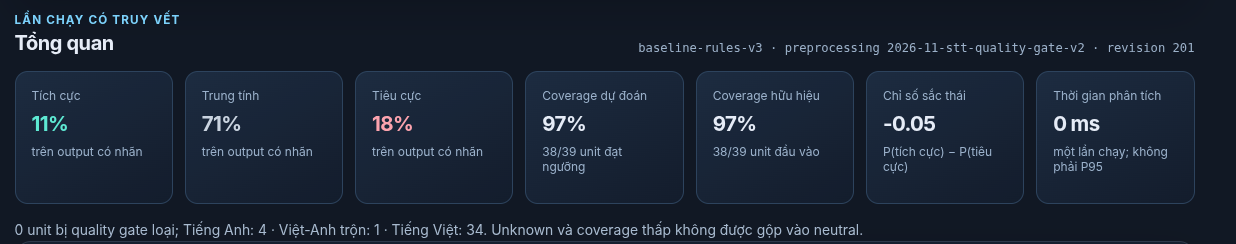
\includegraphics[width=\linewidth]{pictures/experiments/exp02_dashboard_overview.png}
  \caption{Tổng quan aggregate của run pilot: phân bố output, coverage, polarity và version xử lý.}
  \label{fig:experiment-result-02-overview}
\end{figure}

\begin{figure}[H]
  \centering
  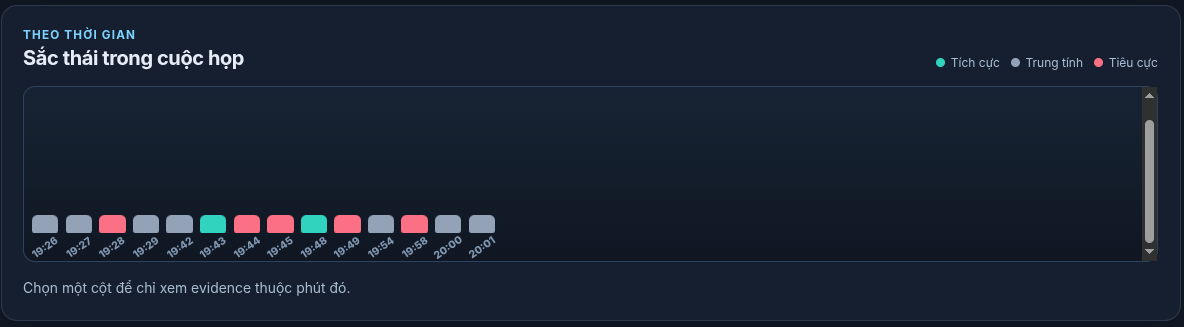
\includegraphics[width=\linewidth]{pictures/experiments/exp02_dashboard_timeline.png}
  \caption{Timeline aggregate của run pilot; màu biểu diễn output theo cửa sổ thời gian, không phải đánh giá người nói.}
  \label{fig:experiment-result-02-timeline}
\end{figure}

Snapshot pilot hỗ trợ quan sát rằng giao diện đã hiển thị dữ liệu sau khi bot tham gia, gồm quality gate, gom unit, output adapter, coverage/\texttt{unknown} và timeline. Nó chưa đủ để xác nhận độc lập một E2E UAT pass trên Jitsi vì thiếu bundle E2. Việc giao diện ẩn 36 segment với nhãn nhiễu và hiển thị một unit trộn ngôn ngữ không có prediction cho thấy chất lượng STT, segmentation và multilingual routing vẫn là rủi ro cần đo riêng. Các ảnh transcript/evidence theo đơn vị và ảnh Jitsi có nội dung hoặc định danh participant không được đưa nguyên ảnh vào khóa luận.

Do không có nhãn tham chiếu đã khóa, reference transcript hoặc lặp độc lập, pilot không chứng minh accuracy/Macro-F1, WER/CER, độ đúng diarization, hiểu ngữ cảnh hay hiệu quả đa ngôn ngữ. Đợt đo tiếp theo cần tách scene/Meeting ID, ghi timestamp bot join và STT, khóa self-label/peer-label trước khi xem prediction, rồi tạo evidence bundle đã redaction cho từng điều kiện.

\section{Kịch bản lỗi và giới hạn triển khai}

Kịch bản vận hành phải gồm backend/worker restart, Valkey unavailable, webhook chữ ký sai/timestamp hết hạn/event ID trùng, transcript revision muộn và dashboard mất kết nối SSE. Mỗi kịch bản ghi input, HTTP status kỳ vọng, database/outbox state, cách recovery, bằng chứng pass/fail và cleanup. Với lỗi Vexa hoặc transcription, dashboard chỉ hiển thị trạng thái/lỗi có thể hành động; không được suy đoán nội dung cuộc họp đã nhận đủ.

Một UAT chưa là user study. Nếu sau này đo trải nghiệm người dùng, protocol phải có participant criteria, consent, task, phiên bản dashboard, tiêu chí completion và kế hoạch xử lý phản hồi. Không dùng dashboard để suy luận trầm cảm, năng lực, hiệu suất hay quyết định nhân sự. Coverage cũng không chứng minh transcript đúng hoặc output sentiment đúng; đánh giá ASR/model chỉ thuộc một đề tài khác có dataset hợp pháp và protocol riêng.

\section{Biên bản bằng chứng và điều kiện kết luận}

Mỗi run kiểm chứng có Evidence ID duy nhất, ví dụ \texttt{EVID-20261026-UAT01}. Bundle cục bộ trong kho evidence của dự án gồm command, exit code, stdout/stderr, environment redaction-safe, manifest và ảnh UAT đã che dữ liệu. Có thể dùng \texttt{capture-evidence.sh} cho unit/integration; UAT dashboard ghi bổ sung output \texttt{dashboard-acceptance.sh}. Nếu không có bundle đầy đủ, báo cáo phải ghi \emph{chưa đo} thay vì điền kết quả.

\begin{table}[H]
\centering
\caption{Nội dung tối thiểu của evidence bundle kiểm chứng ứng dụng}
\label{tab:application-evidence-bundle}
\begin{tabularx}{\linewidth}{p{0.29\linewidth}p{0.38\linewidth}X}
\toprule
Trường & Nội dung & Nguồn \\ \midrule
Định danh & Evidence ID, thời gian ICT, người chạy, PASS/FAIL & \texttt{manifest.md} \\
Phiên bản/môi trường & Git commit, Docker/Compose, image digest nếu có, OS/CPU & \texttt{environment.\allowbreak txt} \\
Lệnh/kết quả & Command đầy đủ, exit code, stdout/stderr & \texttt{commands.txt}, \texttt{exit-code.txt}, \texttt{stdout.log} \\
Dữ liệu/quyền riêng tư & Fixture synthetic hoặc consent áp dụng; redaction đã thực hiện & \texttt{manifest.md} \\
Truy vết dashboard & Run ID, version, preprocessing, revision, coverage, batch duration & API result đã redaction hoặc output UAT \\
Kiểm UI & UUID/run đúng, evidence/timeline, SSE hoặc lý do chưa kiểm & Ảnh đã redaction và checklist \\
Giới hạn/failure & Điểm fail, recovery, claim được phép nêu & \texttt{manifest.md} \\
\bottomrule
\end{tabularx}
\end{table}

Khi B1--B3 pass, kết luận được phép nêu là deployment nội bộ và pipeline synthetic hoạt động theo hợp đồng đã mô tả. Khi B4--B6 có consent và evidence đầy đủ, có thể nêu thêm rằng một luồng người dùng Jitsi đã đi đến dashboard truy vết được trên môi trường đã ghi nhận. Không suy rộng kết luận thành chất lượng ASR/model, hiệu năng tải, SLA, khả năng đa nền tảng hay đánh giá con người.

\chapter{Quyền Riêng Tư, Đạo Đức và An Toàn}
\label{chap:ethics}

\section{Mở đầu và phạm vi đánh giá}
Hệ thống Meeting Intelligence xử lý transcript cuộc họp, siêu dữ liệu cuộc họp và các dự đoán cảm xúc ở mức \emph{analysis unit}. Vì transcript có thể chứa tên riêng, phát biểu cá nhân, ý kiến nghề nghiệp hoặc thông tin nhạy cảm phát sinh trong ngữ cảnh họp, rủi ro không chỉ nằm ở rò rỉ dữ liệu mà còn ở việc diễn giải sai kết quả. Do đó, chương này xem đạo đức như một thuộc tính kiến trúc cần được thiết kế, kiểm thử và vận hành liên tục; không phải là một tuyên bố tuân thủ sau khi hệ thống đã hoàn thành. Cách tiếp cận này phù hợp với các nguyên tắc privacy-by-design \cite{cavoukian2011} và trách nhiệm, minh bạch của hệ thống AI \cite{oecdai2024}.

Phạm vi runtime hiện tại là luồng \emph{Jitsi Meet $\rightarrow$ Vexa $\rightarrow$ STT local $\rightarrow$ FastAPI/PostgreSQL/Valkey $\rightarrow$ worker $\rightarrow$ SSE Dashboard}. Vexa cung cấp sự kiện và bản sao transcript; dịch vụ của đề tài chỉ lưu dữ liệu cần thiết để phân tích, kiểm soát phiên bản transcript và trình bày kết quả. Bộ phân loại đang vận hành là luật xác định \texttt{baseline-rules-v3}; nó không phải công cụ chẩn đoán, không suy luận trạng thái tâm lý của cá nhân và không được dùng để xếp hạng nhân sự, đánh giá học tập, kỷ luật hoặc ra quyết định tự động. Các bộ tích hợp Google Meet, Teams, Zoom và mô hình học máy tùy biến là hướng mở rộng, không phải năng lực đã triển khai.

\section{Mô hình rủi ro và nguyên tắc thiết kế}
Ba lớp đối tượng cần được phân biệt rõ: (i)~dữ liệu gốc, gồm transcript, người nói, thời điểm và trạng thái hiệu đính; (ii)~dữ liệu dẫn xuất, gồm analysis unit, nhãn cảm xúc, confidence, evidence và chỉ số tổng hợp; (iii)~quyết định của con người dựa trên dashboard. Nhãn ở lớp (ii) có thể sai do ASR, ngôn ngữ pha trộn, ngữ cảnh thiếu hoặc quy tắc baseline có độ bao phủ thấp. Vì vậy, một nhãn cảm xúc không được nâng thành kết luận về ý định, năng lực hay sức khỏe của người nói.

Các yêu cầu thiết kế được chuẩn hóa như sau.

\begin{itemize}
  \item \textbf{Giới hạn mục đích:} chỉ phân tích nội dung transcript để hỗ trợ người được ủy quyền xem lại cuộc họp. Mục đích mới, chẳng hạn chấm điểm nhân viên hay theo dõi hành vi, phải được đánh giá lại về pháp lý, đạo đức và kỹ thuật trước khi sử dụng.
  \item \textbf{Tối thiểu hóa dữ liệu:} không chủ đích lưu audio/video thô trong dịch vụ phân tích; chỉ giữ transcript, siêu dữ liệu và evidence tối thiểu cần cho truy vết. Mọi trường dữ liệu phải có lý do xử lý và thời hạn lưu tương ứng.
  \item \textbf{Minh bạch và khả năng phản biện:} dashboard cần hiển thị coverage, trạng thái \texttt{unknown}, evidence, revision transcript, preprocessing và \texttt{model\_version}. Người dùng không nên chỉ nhận một điểm số tổng hợp không có ngữ cảnh.
  \item \textbf{Giám sát bởi con người:} prediction là thông tin hỗ trợ, không kích hoạt hành động bất lợi hay cảnh báo cá nhân tự động. Người đọc phải kiểm tra transcript và ngữ cảnh trước khi đưa ra nhận định.
  \item \textbf{Trách nhiệm giải trình:} phiên bản mô hình, cấu hình tiền xử lý, nguồn sự kiện và kết quả worker được lưu để tái lập một lần chạy. Đây là nền tảng kỹ thuật cho audit, sửa dữ liệu và điều tra sự cố, nhưng chưa tự động tạo ra sự tuân thủ pháp lý.
\end{itemize}

Các nguyên tắc này tương thích với yêu cầu về mục đích cụ thể, mức dữ liệu phù hợp và trách nhiệm của bên kiểm soát dữ liệu trong Nghị định 13/2023/NĐ-CP \cite{decree132023}; đồng thời có tính tham chiếu với GDPR \cite{gdpr2016}. Việc áp dụng cho một tổ chức cụ thể vẫn cần tư vấn pháp lý và đánh giá tác động bảo vệ dữ liệu (DPIA), đặc biệt khi phạm vi xử lý, quốc gia triển khai hoặc đối tượng sử dụng thay đổi.

\section{Consent, quản trị dữ liệu và quyền của chủ thể dữ liệu}
Việc tham dự một cuộc họp không mặc nhiên đồng nghĩa với đồng ý cho việc sao chép transcript, phân tích cảm xúc và lưu kết quả dẫn xuất. Trước khi kết nối nguồn dữ liệu, bên triển khai cần thông báo bằng ngôn ngữ dễ hiểu về nguồn thu thập, mục đích phân tích, loại dữ liệu, nơi lưu trữ, đối tượng có quyền truy cập, thời hạn lưu, đầu mối liên hệ và cách rút hoặc thay đổi sự đồng ý. Consent cần được ghi nhận tách biệt với thông báo lịch họp; khi cơ sở xử lý không phải consent, cơ sở đó cũng cần được xác định và rà soát theo thẩm quyền pháp lý phù hợp \cite{decree132023}.

Trong nghiên cứu, dữ liệu thật không nên được đưa vào Git, tài liệu công khai, log CI/CD hoặc bộ kiểm thử. Các smoke test của đề tài sử dụng fixture tổng hợp và xóa dữ liệu kiểm thử sau khi xác nhận kết quả. Nếu cần dùng transcript thật để đánh giá, cần có quy trình tuyển chọn, khử định danh, phân quyền và phê duyệt đạo đức riêng. Người vận hành cũng cần xác định rõ vai trò giữa tổ chức sở hữu cuộc họp, nhà cung cấp nền tảng họp, Vexa và dịch vụ phân tích; không giả định rằng điều khoản của một nền tảng tự động bao phủ toàn bộ chuỗi xử lý tiếp theo.

\section{Kiểm soát dữ liệu theo vòng đời hệ thống}
Thiết kế hiện tại tạo một số điểm kiểm soát hữu ích, nhưng các điểm đó không thay thế một chương trình bảo vệ dữ liệu hoàn chỉnh.

\begin{description}
  \item[Thu thập và nhập liệu.] FastAPI nhận webhook Vexa có kiểm tra HMAC SHA-256, timestamp và cơ chế chống gửi lặp; dashboard không nắm API key của Vexa. Jitsi là adapter runtime hiện tại; khi bổ sung Google Meet, Teams hoặc Zoom, mỗi adapter phải được đánh giá lại về scope OAuth, webhook, dữ liệu nhận được và điều khoản nền tảng.
  \item[Lưu trữ và xử lý.] PostgreSQL là nguồn dữ liệu chuẩn cho meeting, revision transcript, analysis run và evidence; Valkey chỉ dùng cho hàng đợi/phát tán công việc. Worker chỉ phân tích segment cuối cùng, không bị thu hồi và đã qua quality gate. Việc bỏ các đoạn không đủ điều kiện hoặc gán \texttt{unknown} làm giảm nguy cơ tạo nhãn giả, nhưng không xóa bỏ thiên lệch từ ASR hay dữ liệu đầu vào.
  \item[Truy cập và trình bày.] Dashboard nhận cập nhật qua SSE; trong cấu hình phát triển, backend và dashboard được bind vào loopback. Cơ chế định danh hiện có \texttt{X-App-User-Id} chỉ phục vụ phát triển, chưa phải authentication/authorization đủ cho môi trường thật. Triển khai thực tế cần TLS đầu cuối, SSO/OIDC hoặc cơ chế tương đương, RBAC theo workspace/owner, quản lý secret, audit log và kiểm soát xuất dữ liệu.
  \item[Lưu giữ và xóa.] Dự án đã lưu revision và evidence để truy vết, nhưng chưa triển khai retention schedule, workflow export/correction/deletion, xóa bản sao lưu hay chứng minh xóa dữ liệu. Đây là các hạng mục bắt buộc phải được thiết kế và kiểm thử trước khi xử lý dữ liệu thật lâu dài; không được suy diễn rằng việc không lưu audio/video đồng nghĩa không còn rủi ro từ transcript.
\end{description}

\section{Công bằng, độ tin cậy và diễn giải kết quả}
Độ chính xác của suy luận cảm xúc phụ thuộc vào chất lượng nhận dạng tiếng nói, phương ngữ, chuyển mã ngôn ngữ, thuật ngữ chuyên môn, số người nói và phần ngữ cảnh còn thiếu. Một mô hình hoặc rule được đánh giá tốt trên một tập dữ liệu không tự động công bằng với các nhóm người dùng khác; việc báo cáo chỉ một accuracy chung có thể che khuất sai số theo ngôn ngữ hoặc điều kiện âm thanh. Do đó, khi triển khai mô hình học máy tùy biến trong tương lai, tập đánh giá cần được mô tả bằng \emph{datasheet} \cite{gebru2021}, báo cáo theo lát cắt phù hợp và xem xét calibration, coverage, false positive/false negative thay vì chỉ tối ưu một chỉ số tổng hợp.

Ở MVP, \texttt{baseline-rules-v3} được lựa chọn vì tính xác định và dễ audit, không phải vì đã chứng minh vượt trội về chất lượng. \texttt{Confidence} của output không được diễn giải như xác suất một người ``có cảm xúc tiêu cực''; \texttt{unknown} và low coverage là kết quả hợp lệ cần hiển thị rõ. Dashboard không được biến tổng hợp theo speaker thành bảng xếp hạng, tín hiệu giám sát hoặc cơ sở cho quyết định có hậu quả. Các giới hạn này giúp tránh vòng phản hồi, hiệu ứng bị giám sát và việc dùng hệ thống vượt quá mục tiêu nghiên cứu ban đầu.

\section{Ranh giới với an toàn và sức khỏe tâm thần}
Sentiment trong transcript khác với sàng lọc hoặc chẩn đoán lâm sàng. Những công cụ như PHQ-9 có quy trình thẩm định riêng \cite{kroenke2001}, còn tiêu chuẩn chẩn đoán yêu cầu đánh giá chuyên môn và ngữ cảnh lâm sàng \cite{dsm5}. Vì vậy, hệ thống không được suy luận trầm cảm, nguy cơ tự hại hay tình trạng sức khỏe tâm thần từ nhãn cảm xúc, keyword hoặc confidence. Không có tính năng cảnh báo khủng hoảng tự động trong phạm vi đề tài.

Nếu nghiên cứu trong tương lai mở rộng sang tự hại hoặc suicidality, công việc phải dừng trước khi thu thập/triển khai cho đến khi có phê duyệt ethics, người phụ trách chuyên môn lâm sàng, quy trình phản ứng khẩn cấp, cơ chế chuyển tuyến, đánh giá false alarm/missed detection và bảo vệ người tham gia. Keyword alert đơn thuần không phải là can thiệp an toàn.

\section{Trạng thái hiện tại và điều kiện trước triển khai thực tế}
MVP đã có provenance cho prediction (segment ID, revision, timestamp, preprocessing version và model version), quality gate, webhook signing, tách dashboard khỏi Vexa key và nguyên tắc không tự động ra quyết định. Tuy nhiên, hệ thống \textbf{chưa} tuyên bố tuân thủ GDPR, EU AI Act, Nghị định 13/2023/NĐ-CP hay bất kỳ khuôn khổ nào khác; chưa có DPIA, review pháp lý, consent-management, RBAC/SSO sản xuất, retention/deletion workflow, audit trail hoàn chỉnh hoặc đánh giá fairness trên dữ liệu thật.

Trước khi vận hành ngoài phạm vi MVP, nhóm triển khai cần tối thiểu: xác lập data controller/processor và mục đích xử lý; hoàn tất DPIA và chính sách consent/retention; kiểm thử phân quyền, TLS, backup/restore và quy trình xóa; công bố hướng dẫn sử dụng cùng ranh giới diễn giải; lập quy trình báo cáo sự cố, phản hồi khiếu nại và đánh giá định kỳ model/data drift. Các điều kiện này biến nguyên tắc đạo đức thành tiêu chí nghiệm thu hệ thống có thể kiểm chứng, thay vì chỉ là cam kết trong tài liệu.

Các ràng buộc trên cũng định nghĩa phạm vi của kết luận nghiên cứu ở Chương~\ref{chap:conclusion}: MVP chỉ được kết luận về thiết kế, implementation và cơ chế tạo evidence; snapshot E1 hoặc bundle synthetic lịch sử không là bằng chứng cho một luồng Jitsi E2E hiện tại. Không được kết luận về hiệu quả lâm sàng, chất lượng sentiment trên dữ liệu thật hay mức độ tuân thủ pháp lý. Việc liên kết yêu cầu đạo đức với tiêu chí nghiệm thu kỹ thuật giúp bảo đảm mỗi năng lực mở rộng đều có thể được đánh giá về lợi ích, rủi ro và bằng chứng vận hành trước khi được đưa vào sử dụng.

\chapter{Kết Luận và Hướng Phát Triển}
\label{chap:conclusion}

\section{Tổng kết nghiên cứu}
Khóa luận tiếp cận bài toán phân tích sentiment trên transcript họp như một bài toán \emph{thiết kế, hiện thực và kiểm chứng artefact hệ thống}, thay vì chỉ huấn luyện một bộ phân loại. Cách tiếp cận này phù hợp với nghiên cứu khoa học thiết kế trong hệ thống thông tin: artefact phải giải quyết một lớp vấn đề xác định và được đánh giá bằng bằng chứng phù hợp với mục tiêu của nó \cite{hevner2004}. Trong phạm vi đó, đề tài đã xây dựng MVP cho luồng \emph{Jitsi Meet $\rightarrow$ Vexa $\rightarrow$ STT local $\rightarrow$ FastAPI/PostgreSQL/Valkey $\rightarrow$ worker $\rightarrow$ SSE Dashboard}.

Đóng góp chính của artefact là xác lập một đường đi dữ liệu có thể truy vết: transcript được tiếp nhận và version hóa; quality gate và language routing quyết định dữ liệu có đủ điều kiện suy luận; các segment được ghép thành analysis unit có ranh giới speaker/thời gian; worker tách khỏi API thực hiện phân tích bất đồng bộ; PostgreSQL lưu nguồn dữ liệu chuẩn, run, prediction và evidence; còn dashboard nhận aggregate/evidence qua SSE. Việc gắn prediction với segment ID, transcript revision, preprocessing version và model version làm cho một kết quả có thể được kiểm tra lại khi input hoặc cấu hình thay đổi. Đây là đóng góp về khả năng audit và tích hợp, không phải tuyên bố rằng mọi dự đoán đều đúng.

Runtime đã hiện thực là \texttt{baseline-rules-v3}, đặt sau classifier adapter để kiểm tra hợp đồng xử lý đầu cuối một cách xác định và dễ truy vết. Thiết kế adapter giữ chỗ cho PhoBERT hoặc custom model trong tương lai, nhưng PhoBERT không phải kết quả đã đạt của MVP. Tương tự, Jitsi thông qua Vexa/STT local là adapter runtime hiện hành; Google Meet, Teams và Zoom là phương án kiến trúc mở rộng. Sự phân biệt giữa năng lực đã triển khai và phương án đề xuất là cần thiết để tránh nợ kỹ thuật và các tuyên bố vượt quá bằng chứng thực nghiệm \cite{sculley2015}.

\section{Bằng chứng và phạm vi kết luận}
Chương~\ref{chap:experiments} đã tách năng lực của mã nguồn, quan sát giao diện và evidence tái lập được khỏi đánh giá khoa học của ASR, mô hình và trải nghiệm người dùng. Mã nguồn có test đơn vị cho quality gate, unit builder, service và Vexa parser; smoke pipeline có fixture tổng hợp cho đường đi API--PostgreSQL--Valkey--worker--analytics; các script readiness kiểm tra khả năng tiếp cận service. Kho evidence có bundle integration synthetic \texttt{EVID-20261018-INT02} ở cấu hình \texttt{baseline-rules-v2}/\texttt{2026-09-v1}; còn hai snapshot Dashboard ngày 15/11/2026 là quan sát E1. Vì vậy, luận văn chỉ kết luận rằng artefact có cơ chế kiểm chứng integration và lưu vết được hiện thực; không coi snapshot hay bundle cũ là PASS cho runtime \texttt{baseline-rules-v3} hiện tại hoặc cho Jitsi E2E.

Ngược lại, khóa luận không báo cáo và không suy diễn F1/accuracy sentiment, WER/CER ASR, calibration, latency percentile, throughput, SLA, khả năng chịu tải, hiệu quả PhoBERT hay custom model. Các số lượng segment/unit, coverage và phân bố nhãn ở Chương~\ref{chap:experiments} chỉ là trạng thái giao diện của snapshot E1, không phải ước lượng chất lượng. Không có corpus transcript họp được gán nhãn, benchmark đa mô hình, load test hoặc user study hoàn chỉnh. Mọi bảng định lượng về chất lượng hoặc hiệu năng chỉ được điền sau một run có commit/image, manifest dữ liệu, cấu hình redaction, log và evidence bundle tương ứng. Đây là điều kiện để kết quả sau này có thể tái lập và phản biện.

\section{Ý nghĩa đạo đức và vận hành}
Giá trị của hệ thống không nằm ở một điểm sentiment tổng hợp mà ở khả năng đặt điểm đó trong ngữ cảnh và thể hiện sự không chắc chắn. \texttt{unknown}, rejected unit, coverage thấp và evidence không phải lỗi giao diện cần che giấu, mà là các tín hiệu giúp người dùng tránh diễn giải quá mức. Theo Chương~\ref{chap:ethics}, sentiment của transcript không phải suy luận về năng lực, hành vi hay sức khỏe tâm thần của người nói. Dashboard không được dùng cho xếp hạng nhân sự, đánh giá học tập, kỷ luật hay quyết định tự động.

MVP đã có một số kiểm soát kỹ thuật ban đầu như webhook HMAC, deduplication, provenance và tách dashboard khỏi Vexa key. Tuy nhiên, các kiểm soát đó không đồng nghĩa hệ thống đã tuân thủ quy định. Trước khi xử lý dữ liệu thật trong môi trường vận hành, cần hoàn tất DPIA/review pháp lý, consent management, authentication và authorization sản xuất, TLS, retention/deletion, audit log, backup/restore và quy trình ứng phó sự cố. Privacy-by-design cần được duy trì suốt vòng đời hệ thống \cite{cavoukian2011}; model card và tài liệu vận hành cũng cần ghi rõ mục đích, giới hạn, dữ liệu đánh giá và trường hợp không nên sử dụng \cite{mitchell2019}.

\section{Hạn chế}
Các giới hạn quan trọng của nghiên cứu gồm:

\begin{itemize}
  \item \textbf{Giới hạn dữ liệu và mô hình:} chưa có dataset sentiment đúng miền họp, protocol gán nhãn, split theo meeting, benchmark hoặc artifact model được promote vào serving. Các notebook phân loại trầm cảm nhị phân ngoài miền họp không phải bằng chứng cho sentiment transcript và không được ngoại suy sang sàng lọc lâm sàng.
  \item \textbf{Giới hạn nguồn và tích hợp:} Jitsi--Vexa--STT local là runtime được cấu hình cho demo/UAT, nhưng chưa có evidence E2 cho Jitsi E2E hiện tại; chưa có adapter vận hành cho Google Meet, Teams hoặc Zoom; chưa có E2E production với transcript thật có consent, endpoint HTTPS công khai và bằng chứng vận hành dài hạn.
  \item \textbf{Giới hạn hạ tầng:} Docker Compose hiện phục vụ MVP cục bộ; chưa chứng minh high availability, disaster recovery, autoscaling, quan sát tập trung hoặc resilience dưới tải và fault injection.
  \item \textbf{Giới hạn bảo vệ dữ liệu:} định danh bằng \texttt{X-App-User-Id} là cơ chế phát triển; hệ thống chưa có SSO/RBAC production, consent/retention/deletion workflow và đánh giá fairness trên dữ liệu thực.
\end{itemize}

\section{Hướng phát triển có thể kiểm chứng}
Hướng mở rộng nên được triển khai theo các mốc có điều kiện nghiệm thu rõ ràng, thay vì thay thế baseline bằng một model phức tạp mà không có bằng chứng.

\begin{enumerate}
  \item \textbf{Chuẩn hóa dữ liệu và đánh giá:} xây dựng corpus transcript họp có consent, guideline nhãn, annotator độc lập, split theo meeting và test set khóa. Báo cáo datasheet, phân bố lớp, agreement, Macro-F1 theo lớp, coverage, calibration và error analysis; không dùng test set để tuning \cite{gebru2021,artstein2008}.
  \item \textbf{Vòng đời model:} đóng gói artifact cùng tokenizer, preprocessing, label mapping, threshold, dependency lockfile, evaluation report và model card. MLflow tracking/registry, shadow run và promotion policy là kiến trúc đề xuất để so sánh ứng viên với \texttt{baseline-rules-v3}, không phải service đang vận hành trong MVP.
  \item \textbf{Đo lường hệ thống:} thiết kế workload đại diện, đo latency P50/P95/P99, throughput, queue lag, retry/failure rate, tài nguyên và recovery sau sự cố. Kết quả phải ghi rõ hardware, image, cấu hình và thời điểm chạy trước khi công bố SLA hoặc đặc tính ``gần thời gian thực'' định lượng.
  \item \textbf{Mở rộng tích hợp an toàn:} thêm Google Meet, Teams hoặc Zoom qua adapter contract thống nhất; với mỗi nguồn, kiểm tra OAuth/webhook scope, signature, retry, revision, quyền dữ liệu và consent trước khi nối vào pipeline.
  \item \textbf{Vận hành có trách nhiệm:} hoàn thiện quyền truy cập, retention, deletion, audit, sao lưu/khôi phục, quy trình khiếu nại/sự cố và đánh giá drift/fairness định kỳ. Mọi mở rộng sang safety hoặc sức khỏe tâm thần phải là nghiên cứu riêng có ethics approval, giám sát lâm sàng và protocol phản ứng phù hợp.
\end{enumerate}

\section{Lời kết}
MVP cho thấy một hệ thống phân tích transcript có trách nhiệm phải quản lý đồng thời dữ liệu, ngữ cảnh, bất định và khả năng truy vết; việc thay bộ phân loại chỉ là một phần của bài toán. Nền tảng đã xây dựng tạo điều kiện cho các thực nghiệm NLP tiếng Việt trong họp trực tuyến ở bước tiếp theo, với nguyên tắc không biến tín hiệu ngôn ngữ thành kết luận về con người và không biến thiết kế đề xuất thành kết quả đã được chứng minh.


%----------------------------------------------------------------
% BIBLIOGRAPHY
%----------------------------------------------------------------
\cleardoublepage
\phantomsection
\addcontentsline{toc}{chapter}{Tài liệu tham khảo}
\bibliographystyle{IEEEtran}
\bibliography{config/references}

%----------------------------------------------------------------
% APPENDICES
%----------------------------------------------------------------
% \appendix
% % chapters/appendix.tex
% Bỏ comment \appendix và % chapters/appendix.tex
% Bỏ comment \appendix và % chapters/appendix.tex
% Bỏ comment \appendix và \input{chapters/appendix} trong main.tex khi cần in phụ lục.

\chapter{Artefact, Phạm Vi và Khả Năng Tái Lập}
\label{app:artefact}

Phụ lục này mô tả artefact phần mềm tương ứng với các chương thiết kế, kiểm chứng và đạo đức. Nó không thay thế tài liệu vận hành trong thư mục \texttt{source/}, cũng không công bố kết quả thực nghiệm mới. Mục đích là giúp người đọc phân biệt giữa năng lực đã có trong MVP, điều kiện để tái lập một lần chạy, và các hạng mục chỉ mới ở mức hướng phát triển.

\section{Phạm vi runtime hiện tại}
Runtime của MVP là \texttt{baseline-rules-v3}. Luồng đã được hiện thực là:

\begin{center}
\texttt{Jitsi Meet $\rightarrow$ Vexa $\rightarrow$ STT local $\rightarrow$ FastAPI $\rightarrow$ PostgreSQL/outbox $\rightarrow$ Valkey Stream $\rightarrow$ worker $\rightarrow$ SSE Dashboard}.
\end{center}

Vexa là nhà cung cấp bot và transcript; dịch vụ của đề tài sở hữu bản sao transcript, revision, analysis run, prediction, aggregate và dashboard. PostgreSQL là nguồn dữ liệu chuẩn; Valkey Stream chỉ vận chuyển công việc cho worker và không thay thế lưu trữ bền vững. Dashboard chỉ gọi backend, không truy cập Vexa, PostgreSQL, Valkey hoặc API key.

\begin{longtable}{p{0.28\linewidth}p{0.30\linewidth}p{0.32\linewidth}}
\toprule
\textbf{Thành phần} & \textbf{Trạng thái trong MVP} & \textbf{Không được suy diễn} \\
\midrule
\endhead
\bottomrule
\endfoot
Nguồn họp & Jitsi Meet qua Vexa/STT local & Google Meet, Teams hoặc Zoom đã tích hợp \\
Classifier & Luật xác định \texttt{baseline-rules-v3} sau adapter & PhoBERT/custom model đã fine-tune hoặc tốt hơn baseline \\
Phân phối kết quả & REST analytics và SSE từ FastAPI tới dashboard & WebSocket, cảnh báo tự động hoặc quyết định tự động \\
Hạ tầng & Docker Compose cục bộ, PostgreSQL, Valkey, backend, worker, Nginx dashboard & HA, autoscaling, Kubernetes, SLO/SLA hay production security hoàn chỉnh \\
Quyền truy cập & \texttt{X-App-User-Id} phục vụ development; ownership được kiểm tra trong API & SSO, JWT/OIDC hoặc RBAC production \\
\end{longtable}

\section{Cấu trúc source và cấu hình}
Entry point của artefact là thư mục \texttt{source/}. Chỉ \texttt{source/compose.yaml} và \texttt{source/src/} là đường build/chạy ứng dụng hiện hành; thư mục \texttt{meeting-intelligence-backend/} được giữ lại trong giai đoạn chuyển đổi và không dùng cho demo mới.

\begin{lstlisting}[style=bashstyle, caption={Cấu trúc rút gọn của artefact}]
source/
├── compose.yaml                 # application Compose
├── settings.env.example         # mẫu cấu hình, có thể commit
├── settings.env                 # secret cục bộ, không commit
├── src/backend/                 # FastAPI, worker, test, Dockerfile
├── src/dashboard/               # static dashboard và Nginx
├── scripts/                     # bootstrap, verify, smoke, audit
└── vexa/                        # Vexa meetings/transcript-only self-host
\end{lstlisting}

\texttt{settings.env} chứa URL PostgreSQL/Valkey, port, \texttt{MODEL\_VERSION}, \texttt{PREPROCESSING\_VERSION}, Vexa API base/key, webhook URL và webhook secret. File này không được đưa vào Git, log, image, dashboard hoặc evidence bundle. Dashboard và backend chỉ bind loopback ở cấu hình MVP; khi công khai dịch vụ cần reverse proxy TLS, quản lý secret và xác thực/ủy quyền production như đã nêu ở Chương~\ref{chap:infrastructure}.

\section{Quy trình khởi động và kiểm chứng}
Máy chạy cần Docker Engine và Docker Compose v2. Vexa self-host còn cần Docker Engine phiên bản phù hợp cùng transcription credential/service. Các lệnh sau là quy trình tham chiếu; người vận hành phải tạo secret và cấu hình Vexa trước khi khởi động application.

\begin{lstlisting}[style=bashstyle, caption={Khởi động application và kiểm tra reachability}]
cd source
./scripts/bootstrap.sh
# Chỉnh sửa settings.env cục bộ; không commit file này.

# Khởi động Vexa meetings-only và tạo API key theo tài liệu source/README.md.
docker compose --env-file settings.env config
docker compose --env-file settings.env up -d --build
./scripts/verify.sh
./scripts/runtime-status.sh
\end{lstlisting}

\texttt{verify.sh} chỉ kiểm tra \texttt{docker compose ps}, \texttt{/ready} và HTML dashboard trên loopback. \texttt{runtime-status.sh} lập biên bản read-only về container, port và readiness mà không in credential, transcript hoặc environment của container. Hai script chứng minh reachability tại thời điểm chạy, không phải load test, security assessment hay bằng chứng chất lượng model.

Kiểm tra pipeline nội bộ dùng fixture tổng hợp, không gọi Vexa và không dùng transcript thật:

\begin{lstlisting}[style=bashstyle, caption={Smoke test API--queue--worker--analytics}]
cd source
./scripts/smoke-analysis-pipeline.sh
\end{lstlisting}

Script tạo một meeting fixture và hai segment tiếng Việt tổng hợp, yêu cầu final analysis, đợi worker hoàn tất, sau đó kiểm tra \texttt{status=succeeded}, coverage bằng $1$, hai analysis unit và nhãn \textit{positive}/\textit{negative}. Fixture cùng các row phụ thuộc được xóa theo UUID khi script kết thúc. Do input được cố ý chọn để khớp luật baseline, kết quả pass không được báo cáo là accuracy, F1 hoặc benchmark sentiment.

\section{Hợp đồng API của MVP}
Các endpoint dưới đây phản ánh route trong mã nguồn tại thời điểm biên soạn. Ngoại trừ health/readiness và webhook, API meeting yêu cầu định danh caller; \texttt{X-App-User-Id} là cơ chế development, không phải hướng dẫn authentication production. Chi tiết request/response được cung cấp bởi OpenAPI của FastAPI khi service đang chạy.

\begin{longtable}{p{0.12\linewidth}p{0.48\linewidth}p{0.28\linewidth}}
\toprule
\textbf{Method} & \textbf{Endpoint} & \textbf{Mục đích} \\
\midrule
\endhead
\bottomrule
\endfoot
GET & \texttt{/health} & Liveness cơ bản của backend \\
GET & \texttt{/ready} & Readiness; kiểm tra PostgreSQL và Valkey \\
POST & \texttt{/v1/meetings} & Tạo meeting ứng dụng và yêu cầu Vexa spawn bot cho URL Jitsi hợp lệ \\
GET & \texttt{/v1/meetings?limit=...} & Danh sách meeting mới nhất của owner \\
GET & \texttt{/v1/meetings/\{meeting\_id\}} & Trạng thái meeting thuộc owner \\
POST & \texttt{/v1/meetings/\{meeting\_id\}/sync} & Reconcile transcript từ Vexa \\
GET & \texttt{/v1/meetings/\{meeting\_id\}/transcript} & Đọc segment không bị retracted \\
POST & \texttt{/v1/meetings/\{meeting\_id\}/stop} & Yêu cầu dừng bot \\
GET & \texttt{/v1/meetings/\{meeting\_id\}/events} & SSE event phục vụ refresh dashboard \\
POST & \texttt{/v1/meetings/\{meeting\_id\}/analysis?kind=final} & Tạo/queue analysis run \\
GET & \texttt{/v1/meetings/\{meeting\_id\}/analysis} & Đọc analysis run \\
GET & \texttt{/v1/meetings/\{meeting\_id\}/analytics/overview} & KPI và coverage của run hiện hành \\
GET & \texttt{/v1/meetings/\{meeting\_id\}/analytics/timeline} & Tổng hợp theo cửa sổ thời gian \\
GET & \texttt{/v1/meetings/\{meeting\_id\}/analytics/speakers} & Tổng hợp theo speaker \\
GET & \texttt{/v1/meetings/\{meeting\_id\}/analytics/units} & Unit, prediction và evidence \\
POST & \texttt{/v1/webhooks/vexa} & Nhận webhook Vexa; xác minh HMAC, timestamp và event deduplication \\
\end{longtable}

Webhook dùng chữ ký \texttt{sha256(HMAC(secret, timestamp + ``.'' + raw\_body))}; timestamp quá năm phút hoặc chữ ký sai bị từ chối. Endpoint cần một HTTPS URL mà Vexa có thể truy cập. Polling/reconcile transcript vẫn là fallback khi webhook trễ hoặc thất bại; điều này không loại bỏ yêu cầu kiểm thử webhook valid, tampered và replay trong môi trường được cấp consent.

\section{Mẫu evidence bundle cho một lần chạy}
Một lần kiểm chứng chỉ được ghi nhận là pass khi có artefact quan sát được. Bảng~\ref{tab:appendix-evidence} là mẫu tối thiểu để đính kèm cùng báo cáo; tuyệt đối không điền secret hoặc transcript thật.

\begin{table}[H]
\centering
\caption{Mẫu evidence bundle đã redaction}
\label{tab:appendix-evidence}
\begin{tabularx}{\linewidth}{p{0.34\linewidth}X}
\toprule
\textbf{Trường} & \textbf{Giá trị cần ghi} \\
\midrule
Thời điểm, operator và môi trường & UTC, máy/môi trường, mục đích run \\
Phiên bản artefact & Git commit hoặc image digest; version Compose \\
Cấu hình & Tên profile/port/model/preprocessing đã redaction, không có secret \\
Lệnh và kết quả & Command, exit code, vị trí log hoặc CI artifact \\
Dữ liệu & Fixture tổng hợp hoặc bằng chứng consent/approval của E2E thật; không chép transcript vào báo cáo \\
Kết quả pipeline & Meeting UUID, revision, analysis status, accepted/rejected unit, coverage \\
Evidence giao diện & API response đã redaction, ảnh dashboard hoặc SSE event ID nếu phù hợp \\
Giới hạn/failure & Điều kiện chưa đo, retry, lỗi và cách cleanup \\
\bottomrule
\end{tabularx}
\end{table}

\section{Mẫu thông báo và consent trước vận hành}
Đoạn sau là \textbf{mẫu nội dung khởi đầu}, không phải form consent đã triển khai hay tư vấn pháp lý. Tổ chức triển khai phải rà soát với bộ phận pháp chế/DPIA, xác định controller/processor, thời hạn lưu, quyền của chủ thể dữ liệu và cơ sở xử lý phù hợp. Việc tham dự cuộc họp không tự động đồng nghĩa với đồng ý phân tích transcript. Nguyên tắc này nhất quán với tối thiểu hóa dữ liệu, minh bạch và privacy-by-design \cite{decree132023,cavoukian2011}.

\begin{mdframed}[linecolor=accentblue, linewidth=1.0pt, topline=true]
\textbf{Thông báo dự kiến về phân tích transcript cuộc họp}

Cuộc họp có thể sử dụng hệ thống xử lý transcript để hỗ trợ xem lại \emph{nội dung trao đổi}. Hệ thống xử lý transcript, thông tin người nói/thời điểm và kết quả sentiment ở mức đoạn; kết quả không phải chẩn đoán sức khỏe, không dùng để xếp hạng cá nhân hoặc ra quyết định tự động.

Trước khi tham gia, bạn cần được biết: mục đích và phạm vi xử lý; nguồn dữ liệu; người có quyền truy cập; nơi và thời hạn lưu; cách liên hệ để hỏi, rút/điều chỉnh đồng ý hoặc yêu cầu xử lý dữ liệu; cùng các giới hạn của kết quả. Nội dung thông báo, cơ chế ghi nhận consent, thời hạn xóa và quy trình đáp ứng yêu cầu phải được cấu hình và kiểm thử trước khi dùng dữ liệu thật.
\end{mdframed}

\section{Danh mục không thuộc phạm vi MVP}
Các chức năng sau không được mô tả như đã hoàn thành trong luận văn: phát hiện trầm cảm/tự hại, cảnh báo khủng hoảng, Chrome extension, thu audio/video trực tiếp, Chrome/Jitsi integration, fine-tuning PhoBERT, serving ONNX/GPU, MLflow service, benchmark đa mô hình, WER ASR, load/UX study, JWT/SSO/RBAC production, xóa dữ liệu theo SLA, hoặc báo cáo tuân thủ GDPR/EU AI Act/Nghị định 13. Mọi mục mở rộng cần có thiết kế, kiểm thử và bằng chứng riêng trước khi được đưa vào kết quả nghiên cứu hoặc vận hành.
 trong main.tex khi cần in phụ lục.

\chapter{Artefact, Phạm Vi và Khả Năng Tái Lập}
\label{app:artefact}

Phụ lục này mô tả artefact phần mềm tương ứng với các chương thiết kế, kiểm chứng và đạo đức. Nó không thay thế tài liệu vận hành trong thư mục \texttt{source/}, cũng không công bố kết quả thực nghiệm mới. Mục đích là giúp người đọc phân biệt giữa năng lực đã có trong MVP, điều kiện để tái lập một lần chạy, và các hạng mục chỉ mới ở mức hướng phát triển.

\section{Phạm vi runtime hiện tại}
Runtime của MVP là \texttt{baseline-rules-v3}. Luồng đã được hiện thực là:

\begin{center}
\texttt{Jitsi Meet $\rightarrow$ Vexa $\rightarrow$ STT local $\rightarrow$ FastAPI $\rightarrow$ PostgreSQL/outbox $\rightarrow$ Valkey Stream $\rightarrow$ worker $\rightarrow$ SSE Dashboard}.
\end{center}

Vexa là nhà cung cấp bot và transcript; dịch vụ của đề tài sở hữu bản sao transcript, revision, analysis run, prediction, aggregate và dashboard. PostgreSQL là nguồn dữ liệu chuẩn; Valkey Stream chỉ vận chuyển công việc cho worker và không thay thế lưu trữ bền vững. Dashboard chỉ gọi backend, không truy cập Vexa, PostgreSQL, Valkey hoặc API key.

\begin{longtable}{p{0.28\linewidth}p{0.30\linewidth}p{0.32\linewidth}}
\toprule
\textbf{Thành phần} & \textbf{Trạng thái trong MVP} & \textbf{Không được suy diễn} \\
\midrule
\endhead
\bottomrule
\endfoot
Nguồn họp & Jitsi Meet qua Vexa/STT local & Google Meet, Teams hoặc Zoom đã tích hợp \\
Classifier & Luật xác định \texttt{baseline-rules-v3} sau adapter & PhoBERT/custom model đã fine-tune hoặc tốt hơn baseline \\
Phân phối kết quả & REST analytics và SSE từ FastAPI tới dashboard & WebSocket, cảnh báo tự động hoặc quyết định tự động \\
Hạ tầng & Docker Compose cục bộ, PostgreSQL, Valkey, backend, worker, Nginx dashboard & HA, autoscaling, Kubernetes, SLO/SLA hay production security hoàn chỉnh \\
Quyền truy cập & \texttt{X-App-User-Id} phục vụ development; ownership được kiểm tra trong API & SSO, JWT/OIDC hoặc RBAC production \\
\end{longtable}

\section{Cấu trúc source và cấu hình}
Entry point của artefact là thư mục \texttt{source/}. Chỉ \texttt{source/compose.yaml} và \texttt{source/src/} là đường build/chạy ứng dụng hiện hành; thư mục \texttt{meeting-intelligence-backend/} được giữ lại trong giai đoạn chuyển đổi và không dùng cho demo mới.

\begin{lstlisting}[style=bashstyle, caption={Cấu trúc rút gọn của artefact}]
source/
├── compose.yaml                 # application Compose
├── settings.env.example         # mẫu cấu hình, có thể commit
├── settings.env                 # secret cục bộ, không commit
├── src/backend/                 # FastAPI, worker, test, Dockerfile
├── src/dashboard/               # static dashboard và Nginx
├── scripts/                     # bootstrap, verify, smoke, audit
└── vexa/                        # Vexa meetings/transcript-only self-host
\end{lstlisting}

\texttt{settings.env} chứa URL PostgreSQL/Valkey, port, \texttt{MODEL\_VERSION}, \texttt{PREPROCESSING\_VERSION}, Vexa API base/key, webhook URL và webhook secret. File này không được đưa vào Git, log, image, dashboard hoặc evidence bundle. Dashboard và backend chỉ bind loopback ở cấu hình MVP; khi công khai dịch vụ cần reverse proxy TLS, quản lý secret và xác thực/ủy quyền production như đã nêu ở Chương~\ref{chap:infrastructure}.

\section{Quy trình khởi động và kiểm chứng}
Máy chạy cần Docker Engine và Docker Compose v2. Vexa self-host còn cần Docker Engine phiên bản phù hợp cùng transcription credential/service. Các lệnh sau là quy trình tham chiếu; người vận hành phải tạo secret và cấu hình Vexa trước khi khởi động application.

\begin{lstlisting}[style=bashstyle, caption={Khởi động application và kiểm tra reachability}]
cd source
./scripts/bootstrap.sh
# Chỉnh sửa settings.env cục bộ; không commit file này.

# Khởi động Vexa meetings-only và tạo API key theo tài liệu source/README.md.
docker compose --env-file settings.env config
docker compose --env-file settings.env up -d --build
./scripts/verify.sh
./scripts/runtime-status.sh
\end{lstlisting}

\texttt{verify.sh} chỉ kiểm tra \texttt{docker compose ps}, \texttt{/ready} và HTML dashboard trên loopback. \texttt{runtime-status.sh} lập biên bản read-only về container, port và readiness mà không in credential, transcript hoặc environment của container. Hai script chứng minh reachability tại thời điểm chạy, không phải load test, security assessment hay bằng chứng chất lượng model.

Kiểm tra pipeline nội bộ dùng fixture tổng hợp, không gọi Vexa và không dùng transcript thật:

\begin{lstlisting}[style=bashstyle, caption={Smoke test API--queue--worker--analytics}]
cd source
./scripts/smoke-analysis-pipeline.sh
\end{lstlisting}

Script tạo một meeting fixture và hai segment tiếng Việt tổng hợp, yêu cầu final analysis, đợi worker hoàn tất, sau đó kiểm tra \texttt{status=succeeded}, coverage bằng $1$, hai analysis unit và nhãn \textit{positive}/\textit{negative}. Fixture cùng các row phụ thuộc được xóa theo UUID khi script kết thúc. Do input được cố ý chọn để khớp luật baseline, kết quả pass không được báo cáo là accuracy, F1 hoặc benchmark sentiment.

\section{Hợp đồng API của MVP}
Các endpoint dưới đây phản ánh route trong mã nguồn tại thời điểm biên soạn. Ngoại trừ health/readiness và webhook, API meeting yêu cầu định danh caller; \texttt{X-App-User-Id} là cơ chế development, không phải hướng dẫn authentication production. Chi tiết request/response được cung cấp bởi OpenAPI của FastAPI khi service đang chạy.

\begin{longtable}{p{0.12\linewidth}p{0.48\linewidth}p{0.28\linewidth}}
\toprule
\textbf{Method} & \textbf{Endpoint} & \textbf{Mục đích} \\
\midrule
\endhead
\bottomrule
\endfoot
GET & \texttt{/health} & Liveness cơ bản của backend \\
GET & \texttt{/ready} & Readiness; kiểm tra PostgreSQL và Valkey \\
POST & \texttt{/v1/meetings} & Tạo meeting ứng dụng và yêu cầu Vexa spawn bot cho URL Jitsi hợp lệ \\
GET & \texttt{/v1/meetings?limit=...} & Danh sách meeting mới nhất của owner \\
GET & \texttt{/v1/meetings/\{meeting\_id\}} & Trạng thái meeting thuộc owner \\
POST & \texttt{/v1/meetings/\{meeting\_id\}/sync} & Reconcile transcript từ Vexa \\
GET & \texttt{/v1/meetings/\{meeting\_id\}/transcript} & Đọc segment không bị retracted \\
POST & \texttt{/v1/meetings/\{meeting\_id\}/stop} & Yêu cầu dừng bot \\
GET & \texttt{/v1/meetings/\{meeting\_id\}/events} & SSE event phục vụ refresh dashboard \\
POST & \texttt{/v1/meetings/\{meeting\_id\}/analysis?kind=final} & Tạo/queue analysis run \\
GET & \texttt{/v1/meetings/\{meeting\_id\}/analysis} & Đọc analysis run \\
GET & \texttt{/v1/meetings/\{meeting\_id\}/analytics/overview} & KPI và coverage của run hiện hành \\
GET & \texttt{/v1/meetings/\{meeting\_id\}/analytics/timeline} & Tổng hợp theo cửa sổ thời gian \\
GET & \texttt{/v1/meetings/\{meeting\_id\}/analytics/speakers} & Tổng hợp theo speaker \\
GET & \texttt{/v1/meetings/\{meeting\_id\}/analytics/units} & Unit, prediction và evidence \\
POST & \texttt{/v1/webhooks/vexa} & Nhận webhook Vexa; xác minh HMAC, timestamp và event deduplication \\
\end{longtable}

Webhook dùng chữ ký \texttt{sha256(HMAC(secret, timestamp + ``.'' + raw\_body))}; timestamp quá năm phút hoặc chữ ký sai bị từ chối. Endpoint cần một HTTPS URL mà Vexa có thể truy cập. Polling/reconcile transcript vẫn là fallback khi webhook trễ hoặc thất bại; điều này không loại bỏ yêu cầu kiểm thử webhook valid, tampered và replay trong môi trường được cấp consent.

\section{Mẫu evidence bundle cho một lần chạy}
Một lần kiểm chứng chỉ được ghi nhận là pass khi có artefact quan sát được. Bảng~\ref{tab:appendix-evidence} là mẫu tối thiểu để đính kèm cùng báo cáo; tuyệt đối không điền secret hoặc transcript thật.

\begin{table}[H]
\centering
\caption{Mẫu evidence bundle đã redaction}
\label{tab:appendix-evidence}
\begin{tabularx}{\linewidth}{p{0.34\linewidth}X}
\toprule
\textbf{Trường} & \textbf{Giá trị cần ghi} \\
\midrule
Thời điểm, operator và môi trường & UTC, máy/môi trường, mục đích run \\
Phiên bản artefact & Git commit hoặc image digest; version Compose \\
Cấu hình & Tên profile/port/model/preprocessing đã redaction, không có secret \\
Lệnh và kết quả & Command, exit code, vị trí log hoặc CI artifact \\
Dữ liệu & Fixture tổng hợp hoặc bằng chứng consent/approval của E2E thật; không chép transcript vào báo cáo \\
Kết quả pipeline & Meeting UUID, revision, analysis status, accepted/rejected unit, coverage \\
Evidence giao diện & API response đã redaction, ảnh dashboard hoặc SSE event ID nếu phù hợp \\
Giới hạn/failure & Điều kiện chưa đo, retry, lỗi và cách cleanup \\
\bottomrule
\end{tabularx}
\end{table}

\section{Mẫu thông báo và consent trước vận hành}
Đoạn sau là \textbf{mẫu nội dung khởi đầu}, không phải form consent đã triển khai hay tư vấn pháp lý. Tổ chức triển khai phải rà soát với bộ phận pháp chế/DPIA, xác định controller/processor, thời hạn lưu, quyền của chủ thể dữ liệu và cơ sở xử lý phù hợp. Việc tham dự cuộc họp không tự động đồng nghĩa với đồng ý phân tích transcript. Nguyên tắc này nhất quán với tối thiểu hóa dữ liệu, minh bạch và privacy-by-design \cite{decree132023,cavoukian2011}.

\begin{mdframed}[linecolor=accentblue, linewidth=1.0pt, topline=true]
\textbf{Thông báo dự kiến về phân tích transcript cuộc họp}

Cuộc họp có thể sử dụng hệ thống xử lý transcript để hỗ trợ xem lại \emph{nội dung trao đổi}. Hệ thống xử lý transcript, thông tin người nói/thời điểm và kết quả sentiment ở mức đoạn; kết quả không phải chẩn đoán sức khỏe, không dùng để xếp hạng cá nhân hoặc ra quyết định tự động.

Trước khi tham gia, bạn cần được biết: mục đích và phạm vi xử lý; nguồn dữ liệu; người có quyền truy cập; nơi và thời hạn lưu; cách liên hệ để hỏi, rút/điều chỉnh đồng ý hoặc yêu cầu xử lý dữ liệu; cùng các giới hạn của kết quả. Nội dung thông báo, cơ chế ghi nhận consent, thời hạn xóa và quy trình đáp ứng yêu cầu phải được cấu hình và kiểm thử trước khi dùng dữ liệu thật.
\end{mdframed}

\section{Danh mục không thuộc phạm vi MVP}
Các chức năng sau không được mô tả như đã hoàn thành trong luận văn: phát hiện trầm cảm/tự hại, cảnh báo khủng hoảng, Chrome extension, thu audio/video trực tiếp, Chrome/Jitsi integration, fine-tuning PhoBERT, serving ONNX/GPU, MLflow service, benchmark đa mô hình, WER ASR, load/UX study, JWT/SSO/RBAC production, xóa dữ liệu theo SLA, hoặc báo cáo tuân thủ GDPR/EU AI Act/Nghị định 13. Mọi mục mở rộng cần có thiết kế, kiểm thử và bằng chứng riêng trước khi được đưa vào kết quả nghiên cứu hoặc vận hành.
 trong main.tex khi cần in phụ lục.

\chapter{Artefact, Phạm Vi và Khả Năng Tái Lập}
\label{app:artefact}

Phụ lục này mô tả artefact phần mềm tương ứng với các chương thiết kế, kiểm chứng và đạo đức. Nó không thay thế tài liệu vận hành trong thư mục \texttt{source/}, cũng không công bố kết quả thực nghiệm mới. Mục đích là giúp người đọc phân biệt giữa năng lực đã có trong MVP, điều kiện để tái lập một lần chạy, và các hạng mục chỉ mới ở mức hướng phát triển.

\section{Phạm vi runtime hiện tại}
Runtime của MVP là \texttt{baseline-rules-v3}. Luồng đã được hiện thực là:

\begin{center}
\texttt{Jitsi Meet $\rightarrow$ Vexa $\rightarrow$ STT local $\rightarrow$ FastAPI $\rightarrow$ PostgreSQL/outbox $\rightarrow$ Valkey Stream $\rightarrow$ worker $\rightarrow$ SSE Dashboard}.
\end{center}

Vexa là nhà cung cấp bot và transcript; dịch vụ của đề tài sở hữu bản sao transcript, revision, analysis run, prediction, aggregate và dashboard. PostgreSQL là nguồn dữ liệu chuẩn; Valkey Stream chỉ vận chuyển công việc cho worker và không thay thế lưu trữ bền vững. Dashboard chỉ gọi backend, không truy cập Vexa, PostgreSQL, Valkey hoặc API key.

\begin{longtable}{p{0.28\linewidth}p{0.30\linewidth}p{0.32\linewidth}}
\toprule
\textbf{Thành phần} & \textbf{Trạng thái trong MVP} & \textbf{Không được suy diễn} \\
\midrule
\endhead
\bottomrule
\endfoot
Nguồn họp & Jitsi Meet qua Vexa/STT local & Google Meet, Teams hoặc Zoom đã tích hợp \\
Classifier & Luật xác định \texttt{baseline-rules-v3} sau adapter & PhoBERT/custom model đã fine-tune hoặc tốt hơn baseline \\
Phân phối kết quả & REST analytics và SSE từ FastAPI tới dashboard & WebSocket, cảnh báo tự động hoặc quyết định tự động \\
Hạ tầng & Docker Compose cục bộ, PostgreSQL, Valkey, backend, worker, Nginx dashboard & HA, autoscaling, Kubernetes, SLO/SLA hay production security hoàn chỉnh \\
Quyền truy cập & \texttt{X-App-User-Id} phục vụ development; ownership được kiểm tra trong API & SSO, JWT/OIDC hoặc RBAC production \\
\end{longtable}

\section{Cấu trúc source và cấu hình}
Entry point của artefact là thư mục \texttt{source/}. Chỉ \texttt{source/compose.yaml} và \texttt{source/src/} là đường build/chạy ứng dụng hiện hành; thư mục \texttt{meeting-intelligence-backend/} được giữ lại trong giai đoạn chuyển đổi và không dùng cho demo mới.

\begin{lstlisting}[style=bashstyle, caption={Cấu trúc rút gọn của artefact}]
source/
├── compose.yaml                 # application Compose
├── settings.env.example         # mẫu cấu hình, có thể commit
├── settings.env                 # secret cục bộ, không commit
├── src/backend/                 # FastAPI, worker, test, Dockerfile
├── src/dashboard/               # static dashboard và Nginx
├── scripts/                     # bootstrap, verify, smoke, audit
└── vexa/                        # Vexa meetings/transcript-only self-host
\end{lstlisting}

\texttt{settings.env} chứa URL PostgreSQL/Valkey, port, \texttt{MODEL\_VERSION}, \texttt{PREPROCESSING\_VERSION}, Vexa API base/key, webhook URL và webhook secret. File này không được đưa vào Git, log, image, dashboard hoặc evidence bundle. Dashboard và backend chỉ bind loopback ở cấu hình MVP; khi công khai dịch vụ cần reverse proxy TLS, quản lý secret và xác thực/ủy quyền production như đã nêu ở Chương~\ref{chap:infrastructure}.

\section{Quy trình khởi động và kiểm chứng}
Máy chạy cần Docker Engine và Docker Compose v2. Vexa self-host còn cần Docker Engine phiên bản phù hợp cùng transcription credential/service. Các lệnh sau là quy trình tham chiếu; người vận hành phải tạo secret và cấu hình Vexa trước khi khởi động application.

\begin{lstlisting}[style=bashstyle, caption={Khởi động application và kiểm tra reachability}]
cd source
./scripts/bootstrap.sh
# Chỉnh sửa settings.env cục bộ; không commit file này.

# Khởi động Vexa meetings-only và tạo API key theo tài liệu source/README.md.
docker compose --env-file settings.env config
docker compose --env-file settings.env up -d --build
./scripts/verify.sh
./scripts/runtime-status.sh
\end{lstlisting}

\texttt{verify.sh} chỉ kiểm tra \texttt{docker compose ps}, \texttt{/ready} và HTML dashboard trên loopback. \texttt{runtime-status.sh} lập biên bản read-only về container, port và readiness mà không in credential, transcript hoặc environment của container. Hai script chứng minh reachability tại thời điểm chạy, không phải load test, security assessment hay bằng chứng chất lượng model.

Kiểm tra pipeline nội bộ dùng fixture tổng hợp, không gọi Vexa và không dùng transcript thật:

\begin{lstlisting}[style=bashstyle, caption={Smoke test API--queue--worker--analytics}]
cd source
./scripts/smoke-analysis-pipeline.sh
\end{lstlisting}

Script tạo một meeting fixture và hai segment tiếng Việt tổng hợp, yêu cầu final analysis, đợi worker hoàn tất, sau đó kiểm tra \texttt{status=succeeded}, coverage bằng $1$, hai analysis unit và nhãn \textit{positive}/\textit{negative}. Fixture cùng các row phụ thuộc được xóa theo UUID khi script kết thúc. Do input được cố ý chọn để khớp luật baseline, kết quả pass không được báo cáo là accuracy, F1 hoặc benchmark sentiment.

\section{Hợp đồng API của MVP}
Các endpoint dưới đây phản ánh route trong mã nguồn tại thời điểm biên soạn. Ngoại trừ health/readiness và webhook, API meeting yêu cầu định danh caller; \texttt{X-App-User-Id} là cơ chế development, không phải hướng dẫn authentication production. Chi tiết request/response được cung cấp bởi OpenAPI của FastAPI khi service đang chạy.

\begin{longtable}{p{0.12\linewidth}p{0.48\linewidth}p{0.28\linewidth}}
\toprule
\textbf{Method} & \textbf{Endpoint} & \textbf{Mục đích} \\
\midrule
\endhead
\bottomrule
\endfoot
GET & \texttt{/health} & Liveness cơ bản của backend \\
GET & \texttt{/ready} & Readiness; kiểm tra PostgreSQL và Valkey \\
POST & \texttt{/v1/meetings} & Tạo meeting ứng dụng và yêu cầu Vexa spawn bot cho URL Jitsi hợp lệ \\
GET & \texttt{/v1/meetings?limit=...} & Danh sách meeting mới nhất của owner \\
GET & \texttt{/v1/meetings/\{meeting\_id\}} & Trạng thái meeting thuộc owner \\
POST & \texttt{/v1/meetings/\{meeting\_id\}/sync} & Reconcile transcript từ Vexa \\
GET & \texttt{/v1/meetings/\{meeting\_id\}/transcript} & Đọc segment không bị retracted \\
POST & \texttt{/v1/meetings/\{meeting\_id\}/stop} & Yêu cầu dừng bot \\
GET & \texttt{/v1/meetings/\{meeting\_id\}/events} & SSE event phục vụ refresh dashboard \\
POST & \texttt{/v1/meetings/\{meeting\_id\}/analysis?kind=final} & Tạo/queue analysis run \\
GET & \texttt{/v1/meetings/\{meeting\_id\}/analysis} & Đọc analysis run \\
GET & \texttt{/v1/meetings/\{meeting\_id\}/analytics/overview} & KPI và coverage của run hiện hành \\
GET & \texttt{/v1/meetings/\{meeting\_id\}/analytics/timeline} & Tổng hợp theo cửa sổ thời gian \\
GET & \texttt{/v1/meetings/\{meeting\_id\}/analytics/speakers} & Tổng hợp theo speaker \\
GET & \texttt{/v1/meetings/\{meeting\_id\}/analytics/units} & Unit, prediction và evidence \\
POST & \texttt{/v1/webhooks/vexa} & Nhận webhook Vexa; xác minh HMAC, timestamp và event deduplication \\
\end{longtable}

Webhook dùng chữ ký \texttt{sha256(HMAC(secret, timestamp + ``.'' + raw\_body))}; timestamp quá năm phút hoặc chữ ký sai bị từ chối. Endpoint cần một HTTPS URL mà Vexa có thể truy cập. Polling/reconcile transcript vẫn là fallback khi webhook trễ hoặc thất bại; điều này không loại bỏ yêu cầu kiểm thử webhook valid, tampered và replay trong môi trường được cấp consent.

\section{Mẫu evidence bundle cho một lần chạy}
Một lần kiểm chứng chỉ được ghi nhận là pass khi có artefact quan sát được. Bảng~\ref{tab:appendix-evidence} là mẫu tối thiểu để đính kèm cùng báo cáo; tuyệt đối không điền secret hoặc transcript thật.

\begin{table}[H]
\centering
\caption{Mẫu evidence bundle đã redaction}
\label{tab:appendix-evidence}
\begin{tabularx}{\linewidth}{p{0.34\linewidth}X}
\toprule
\textbf{Trường} & \textbf{Giá trị cần ghi} \\
\midrule
Thời điểm, operator và môi trường & UTC, máy/môi trường, mục đích run \\
Phiên bản artefact & Git commit hoặc image digest; version Compose \\
Cấu hình & Tên profile/port/model/preprocessing đã redaction, không có secret \\
Lệnh và kết quả & Command, exit code, vị trí log hoặc CI artifact \\
Dữ liệu & Fixture tổng hợp hoặc bằng chứng consent/approval của E2E thật; không chép transcript vào báo cáo \\
Kết quả pipeline & Meeting UUID, revision, analysis status, accepted/rejected unit, coverage \\
Evidence giao diện & API response đã redaction, ảnh dashboard hoặc SSE event ID nếu phù hợp \\
Giới hạn/failure & Điều kiện chưa đo, retry, lỗi và cách cleanup \\
\bottomrule
\end{tabularx}
\end{table}

\section{Mẫu thông báo và consent trước vận hành}
Đoạn sau là \textbf{mẫu nội dung khởi đầu}, không phải form consent đã triển khai hay tư vấn pháp lý. Tổ chức triển khai phải rà soát với bộ phận pháp chế/DPIA, xác định controller/processor, thời hạn lưu, quyền của chủ thể dữ liệu và cơ sở xử lý phù hợp. Việc tham dự cuộc họp không tự động đồng nghĩa với đồng ý phân tích transcript. Nguyên tắc này nhất quán với tối thiểu hóa dữ liệu, minh bạch và privacy-by-design \cite{decree132023,cavoukian2011}.

\begin{mdframed}[linecolor=accentblue, linewidth=1.0pt, topline=true]
\textbf{Thông báo dự kiến về phân tích transcript cuộc họp}

Cuộc họp có thể sử dụng hệ thống xử lý transcript để hỗ trợ xem lại \emph{nội dung trao đổi}. Hệ thống xử lý transcript, thông tin người nói/thời điểm và kết quả sentiment ở mức đoạn; kết quả không phải chẩn đoán sức khỏe, không dùng để xếp hạng cá nhân hoặc ra quyết định tự động.

Trước khi tham gia, bạn cần được biết: mục đích và phạm vi xử lý; nguồn dữ liệu; người có quyền truy cập; nơi và thời hạn lưu; cách liên hệ để hỏi, rút/điều chỉnh đồng ý hoặc yêu cầu xử lý dữ liệu; cùng các giới hạn của kết quả. Nội dung thông báo, cơ chế ghi nhận consent, thời hạn xóa và quy trình đáp ứng yêu cầu phải được cấu hình và kiểm thử trước khi dùng dữ liệu thật.
\end{mdframed}

\section{Danh mục không thuộc phạm vi MVP}
Các chức năng sau không được mô tả như đã hoàn thành trong luận văn: phát hiện trầm cảm/tự hại, cảnh báo khủng hoảng, Chrome extension, thu audio/video trực tiếp, Chrome/Jitsi integration, fine-tuning PhoBERT, serving ONNX/GPU, MLflow service, benchmark đa mô hình, WER ASR, load/UX study, JWT/SSO/RBAC production, xóa dữ liệu theo SLA, hoặc báo cáo tuân thủ GDPR/EU AI Act/Nghị định 13. Mọi mục mở rộng cần có thiết kế, kiểm thử và bằng chứng riêng trước khi được đưa vào kết quả nghiên cứu hoặc vận hành.


\end{document}
